% \pagenumbering{arabic}
\algdef{SE}[DOWHILE]{Do}{doWhile}{\algorithmicdo}[1]{\algorithmicwhile\ #1}%
\renewcommand{\b}{\mathbf}
% \floatsetup[table]{capposition=top}
% \newfloatcommand{capbtabbox}{table}[][\FBwidth]


\chapter{\TitlechapterIII}
\section{本章引言}

在现代复杂过程工业生产中,对控制性能指标进行优化是不同控制算法、控制系统的首要任务。
% 在冶金、采矿领域等复杂过程工业场景下,浓密机是一种被广泛应用的大型沉降工具,它通过重力沉降作用可以将低浓度的固液混合物进行浓缩形成高浓度的混合物,起到减水、浓缩的作用。
% 在对浓密机进行控制时,底流浓度是核心控制指标。该参量与其他过程监控变量如进料流量、进料浓度、出料流量、泥层高度有着复杂的耦合关系。
% 在大部分的实际生产过程中,浓密机底流浓度的控制一般是操作员根据个人经验,通过对底流流量设定值、絮凝剂流量设定值进行调节,间接地使底流浓度追踪其工艺设定值。但是由于浓密机运行过程具有非线性、多变量、高时滞等特点,操作员难以维持底流浓度持续稳定,浓度存在偏差的底流会导致产品质量退化以及增加工业生产成本。
在大部分的实际生产过程中,复杂工业系统的控制一般是结合局部环路反馈控制器与操作员的个人经验,利用PID等控制算法对底层执行设备的频率、泵速、开度进行调节,间接地使关键指标追踪人为给定的工艺设定值。
但是由于大部分复杂工业系统运行过程具有非线性、多变量、高时滞等特点,操作员难以实时地给出合理的工艺设定值,底层变量之间难以满足线性或单调关系,简单的反馈控制算法难以适应。
当关键指标存在控制偏差时会导致产品质量退化以及增加工业生产成本。

关于复杂过程工业设备优化控制的研究一直是工业界、学术界研究的热点问题。
对于机械结构明确、且能够精确建立动态模型的工业设备,可以采用基于模型的优化控制方法,如:实时优化控制(realtime
optimization, RTO)\cite{Yin2014}、模型预测控制(model predictive
control,MPC)\cite{Kouro2009}等。
但对于机械结构复杂、部分变量难以观测的、动力学方程未知的复杂系统,难以建立准确的数学模型近似其运转机理,导致基于模型的方法无法适用于此类复杂工业设备的控制。
研究人员提出了基于数据驱动的控制方法来实现对此类无模型工业设备的控制。
Dai等\cite{Dai2015}提出了用于解决赤铁矿研磨系统控制问题的数据驱动优化(Data-driven optimization, DDO)控制算法。
Wang等\cite{Wang2016}采用基于数据驱动的自适应评价方法解决连续时间未知非线性系统的鲁棒最优控制问题。

近年来,基于强化学习\cite{Sutton2018}\cite{F.L.LewisD.Vrabie2012}理论的最优控制技术,也称为自适应动态规划(Adaptive dynamic programming, ADP)\cite{Prokhorov1997}\cite{Werbos2008}\cite{Duan:643}技术,是控制领域研究的热点话题。
典型的自适应动态规划算法,如HDP、双启发式动态规划(Dual heuristic
programming,DHP)、动作依赖启发式动态规划(Action dependent
heuristic dynamic programming,
ADHDP)\cite{Werbos2008}等均采用多个神经网络分别对被控系统的动态模型、控制策略、策略评价模型进行建模。此类方法可以在模型未知的情况下以数据驱动的方式在线学习控制策略。
Liu等\cite{Liu2015}提出了一种在线自适应动态规划算法用来解决离散时间多输入多输出仿射系统控制问题,且该方法仅需要训练少量网络参数。
% Liu等\cite{LiuL2017}采用一种基于强化学习的自适应跟踪控制技术解决多输入多输出系统容错控制问题。
Xu等\cite{XuX2017}采用拉普拉斯特征映射算法提取被控系统全局特征,并将该全局特征用于DHP算法中以增强值函数网络的近似能力。
Li等\cite{LI2021109687} 为了消除ADP算法的跟踪误差提出了一种新的值函数表达形式,忽略了效用函数中控制输入的二次项,使得值函数的有界性和收敛性与折扣因子无关。新的值函数形式可以在不给定控制输入设定点的情况下推导出最优控制策略。

% 近年来,利用自适应动态规划方法解决过程工业控制问题也取得很大研究进展。
近年来,自适应动态规划方法也常被用于解决过程工业控制问题。
Wei等\cite{Wei2014}将煤炭气化过程的最优追踪控制转化为双人零和最优控制问题,并采用迭代自适应动态规划方法求解最优控制律,同时给出了收敛稳定性的分析。
Jiang等\cite{Jiang2018}利用穿插学习策略迭代(Interleaved Learning
Policy Iteration,ILPL)实现了对浮选过程操作指标优化的控制,获得了比传统值函数迭代(Value iteration, VI)、策略迭代(Policy iteration, PI)算法更佳的控制效果。
Jiang等\cite{Jiang2019}将强化学习与举升方法结合(lifting technology),实现了对浮选过程设备层与操作层双速率系统的最优控制。
上述算法均使用被控系统实时生成的数据对神经网络进行训练,但其控制器与评价模块的设计均建立在系统数据采样是均匀的这一假设之上,而无法适用于采样间隔非均匀的情况。
另外,上述训练方法没有在模型学习过程中充分利用系统短期内产生的历史轨迹数据,在数据利用率方面存在改进空间。
同时,在工业场景下进行设备在线控制对算法实时性要求较高。
上述方法对于控制量的计算均依托于表征控制策略的神经网络,而对于控制网络的训练将产生较大的时间开销。

为了解决上述问题,本章提出了基于连续时间有模型强化学习的复杂工业系统优化控制方法。该方法首先使用系统离线运行数据建模被控系统的连续时间动态方程,
% 使用本文三、四、五章所述的连续时间动态系统辨识模型
然后在在线控制场景下,采集系统实时数据并执行有模型强化学习过程以训练在线控制策略并调优动态模型。
同时,针对复杂工业系统存在运行缓慢的特性,提出基于梯度迭代优化的控制求解算法,该算法可以在不引入控制网络的情况下高效求解控制输入量,在提升控制精度的同时,避免了训练控制网络的时间消耗。
另外,本章引入了短期经验回放技术\cite{Modares2014}\cite{Mnih2013}对短期内的系统运行轨迹数据进行回放训练,以提升局部状态评价及梯度值拟合的准确性。
最后,实验环节分别将HCNVI控制算法应用于浓密机仿真模型及某矿山深锥浓密机系统,证实了该控制算法在解决底流浓度追踪控制问题时的有效性以及在训练效率、控制精度方面的优越性。




% 为了克服人工控制的缺陷,多种针对浓密机的智能控制算法被提出。
% Xu,Ning等\cite{Xu2015}利用泥层质量平衡模型与专家系统实现了对絮凝剂添加比例与底流流量设定值的控制,
% Chai等\cite{Chai2016}\cite{Wang330}将模糊控制算法与(Proportional
% Integral Differential,
% PID)控制相结合,实现对底流浓度的控制,且最大程度保持底流流量的稳定性。
% Ojeda,P等\cite{Ojeda2014}利用复杂专家系统实现了对于底流浓度与溢流水浊度的控制,并且在实际工业场景获得较好效果。
% 由于浓密机运行机理复杂,难以建立数学模型,难以应用传统控制理论、最优控制算法,大部分浓密机控制算法都是基于人工设计的专家系统或手工制定模糊控制器中的规则库

% 通过归纳现有的浓密机控制手段,可以发现由于浓密机运行机理复杂,难以建立数学模型,难以应用传统控制理论、最优控制算法,大部分的控制算法都是基于人工设计的专家系统或手工制定模糊控制器中的规则库,并辅助以传统的比例积分控制手段实现对底流泵速、絮凝剂泵速的控制。此类方法过度依赖人工经验、缺乏自适应性。

% %本章提出了基于强化学习\cite{Sutton2018}\cite{F.L.LewisD.Vrabie2012}的浓密机在线控制算法。
% 近年来,基于强化学习\cite{Sutton2018}\cite{F.L.LewisD.Vrabie2012}理论的最优控制技术(也称为自适应动态规划(Adaptive
% dynamic programming,
% ADP)\cite{Prokhorov1997}\cite{Duan:643}\cite{Jiang2018}\cite{Liu2015}
% \cite{XuX2017}\cite{LiuL2017}),在解决飞行器控制\cite{helicopters}、车辆控制\cite{Vehicles}等方面取得了很大的进展。
% 并且在过程工业控制领域中,采用强化学习方法解决工业控制场景下指标设定值追踪与智能优化控制问题的思想也催生出诸多研究成果\cite{Jiang2018}\cite{Li2018}\cite{Jiang2019}\cite{Xue2019}。
% 尽管复杂过程工业场景下外部环境因素扰动频繁、设备运行过程复杂且难以建立数学模型对其生产过程进行准确的描述,但强化学习算法具有自适应、不依赖于精确数学模型的特点,因此可以作为一种解决复杂过程工业设备优化控制问题的有效手段。

% 本章提出了基于强化学习的浓密机在线控制算法。通过设计融合评价网络与模型网络的双网结构实现对浓密机底流泵速和絮凝剂泵速的控制。
% 评价网络用于拟合折扣累计代价函数,模型网络用于对生产过程进行建模与预测。
% 为了增加控制模型在噪音量改变下的收敛速度,相比于传统HDP算法,本章在双网结构中去掉了动作网络。
% 前人研究表明\cite{Luo2016}\cite{Padhi2006},在启发式动态规划类算法中,去掉动作网络可以有效减少模型训练时间。但是在某些复杂系统控制问题中,去除动作网络会使模型难以拟合复杂策略函数,最终引起控制效果变差。
% 本章采用迭代梯度优化算法求解控制输入量,该方法不仅保留了无动作网络类ADP方法在训练时间上的优势,并且由于浓密机系统具有运行缓慢的特性,该方法在浓密机控制问题上也获得了相比传统方法更佳的控制效果。
% 此外,由于浓密机具有运行缓慢、状态迁移滞后的特点,为了维持评价网络的局部梯度差异以增强控制模型的收敛速度,本章提出了短期经验回放技术\cite{Modares2014}\cite{Mnih2013}以对短期内的系统运行轨迹数据进行回放训练。
% 实验证明该技术有效增强了算法收敛稳定性,且在其他ADP类在线控制算法中具有通用性。

本章主要贡献总结如下:
\begin{itemize}[nosep]
\item  提出了一种基于连续时间有模型强化学习的复杂工业系统控制算法——启发式评价网络值迭代算法
(Heuristic critic network value iteration,HCNVI)。该算法能够利用非均匀系统采样数据在线训练连续时间域的评价网络、模型网络,并采用梯度优化算法求解系统最优控制输入。
% \item  一种浓密机预测网络训练方法,根据进料噪音项的概率分布,对原始离线数据进行采样构建预测网络训练集,该方法可以有效增强模型网络预测精确度,并对控制模型性能产生促进作用。
\item  提出了一种适用于评价网络训练的短期经验回放技术。训练评价网络时,将短期内系统运行轨迹数据共同用于模型训练,该方法可以有效增强评价网络收敛速度。
\item  通过工业系统仿真实验验证了HCNVI算法在训练时间消耗、控制精度上均优于其他对比方法。
\item  在真实工业场景下,成功将HCNVI算法应用于浓密机控制,有效稳定设备的底流浓度。
\end{itemize}

本章内容组织如下: 
\secref{sec:formulation}对连续时间域下的复杂工业系统的控制过程进行形式化描述。
% \secref{sec:6_hcnvi}介绍了如何基于ODE-Net模型构建浓密机系统运行过程的模型网络。
\secref{sec:6_hcnvi}介绍了HCNVI算法的模型训练及在线控制过程,具体包括基于神经常微分方程的模型网络构建、基于积分强化学习的策略评价、基于随机梯度下降的动作生成、以及用于评价网络训练的短期经验回放。
\secref{sec:experiment}分别通过浓密机仿真实验以及真实工业实验验证本章提出控制模型的有效性。
\secref{sec:conclusion}对本章研究工作进行总结。

% \section{连续时间强化学习形式化描述}
\section{复杂系统无模型控制形式化描述}
\label{sec:formulation}
% Please add the following required packages to your document preamble:
% \usepackage{graphicx}

% \begin{table}[!ht]
% \centering
% \caption{浓密过程示意图中符号解释}
%  %英文标题begin
%     \addtocounter{table}{-1}
%     \vspace{-0.2cm}
%     %\SetEnglishCaption
%     \renewcommand{\tablename}{Table}
%     \caption{Explaination of symbols in illustration of thickening process.}
%     \renewcommand{\tablename}{表}
%     \vspace{0.4cm}
%  %英文标题end
% \begin{tabular}{@{}lll@{}}
% \toprule
% 符号 & 含义 & 单位 \\ \midrule
% DT & 密度变送器 & $kg/m^3$ \\
% FT & 流量变送器 & $m^3/h$ \\
% PT & 压强变送器 & $kPa$ \\
% AT & 浊度变送器 & $ppm$ \\
% LT & 液位变送器 & $m$ \\ \bottomrule
% \end{tabular}
% \label{tab:symble_explain}
% \end{table}
对于一般的复杂工业系统,其系统运行过程的控制效果往往根据某些监测指标的状态进行评价,假定其控制目标为$\b y(t) \in \mathbb{R}^n$。
该指标受控制输入、系统状态参量、及其他外部噪音扰动影响。
本节将系统可控制输入量表示为$\b u(t) \in \mathbb{R}^m$,
将不作为控制目标的系统输出量表示为$\b h(t) \in \mathbb{R}^l$,该参量是表征当前系统状态的重要参量,它可被间接控制但不作为控制过程中的评价项。
由于在部分工业场景中,上游工序产生的物料性质是不可控的。为了使提出的控制模型具有通用性,因此本章引入噪音输入量$\b c(t) \in\mathbb{R}^d$以定义那些会对生产系统产生影响的、可被监测,但无法被控制的监测量。
因此,被控系统可表述为\equref{equ:system_dynamic_dt}形式的非线性系统,其中$f
( \cdot )$为未知非线性函数。
\begin{equation}\label{equ:system_dynamic_dt}
    [\b y ( t_{k + 1} ), \b h(t_{k+1})]^{\rm T} = f ( \b y(t_k), \b u ( t_k ) ,\b c ( t_k ) ,\b h(t_k), t_{k+1}-t_k)
\end{equation}
定义系统状态量$\b s(t)=[\b y(t), \b h(t),\b c(t)]^T$。从连续时间域角度,动态系统可以进一步写成如下形式:
\begin{equation}
\dot{\b{s}}(t)=\frac{d \b{s}(t)}{d t}=\b{f}(\b{s}(t), \b{u}(t))
\end{equation}
函数$\mathbf{f}: \mathbb{R}^{n+m+l+d} \mapsto \mathbb{R}^{n+l+d}$描述了系统当前状态与外部输入量到系统状态导数$\boldsymbol{\dot s}(t)$的映射。
在任意实值时间$t\in R_{+}$的系统状态依赖于初始状态$\b s_0$以及外部输入信号$\b u[0,t)$的无穷小序列。求解过程为:
\begin{equation}
\label{equ:system_dynamic_ct}
\mathbf{s}(t)=\mathbf{s}_{0}+\int_{0}^{t} \mathbf{f}(\mathbf{s}(\tau), \mathbf{u}(\tau)) d \tau,
\end{equation}
其中$\tau$为辅助时间变量。

对于系统运行过程\equref{equ:system_dynamic_ct},本章提出的连续时间域下复杂工业系统控制算法可以根据任意时刻系统状态量$\b s(t)$,实时给出最优的控制输入量$\b u^*(t)$,
使系统输出$y(t)$追踪其设定值$y^*(t)$。另外,为了保证系统运行安全与仪器寿命,控制输入量必须满足一定的限制条件。因此,定义控制系统效用函数为:
\begin{equation}
  \begin{aligned}
    U(t)=&U(\b s(t), \b u(t))\\
    =&\left(\b y(t)-\b y^{*}(t)\right)^{T}Q\left(\b y(t)-\b y^{*}(t)\right)+\left(\b u(t)-{\b u_{\text{mid}}}\right)^{T} R\left(\b u(t)-{\b u_{\text{mid}}}\right)
  \end{aligned}
\label{equ:U}
\end{equation}
效用函数代表了在当前状态$\b s(t)$下,执行控制输入${\b u}(t)$需要承受的代价。$Q$、$R$是对称正定矩阵。$\b u_{\text{mid}}=\dfrac{\b u _ { \max } + \b u _ { \min }}{2}$,$\b u _{\min}$、$\b u _{\max}$分别代表$u(t)$的上限和下限,。

连续时间(CT)控制的目标为在满足控制约束下,最小化效应函数在无穷时间范围下的积分$\int_{t}^{\infty} U(\mathbf{s}(\tau), \mathbf{u}(\tau)) d \tau$。综上本章将其转化为有约束的无穷范围折扣累积代价积分最优化问题:
\begin{equation}
\label{equ:goal}
\begin{aligned}
&{\min_{\b u[t,\infty)}} \quad V(\mathbf{s}(t))=\int_{t}^{\infty} e^{-\frac{\tau-t}{\eta}} U(\mathbf{s}(\tau), \mathbf{u}(\tau)) d \tau \\
& \rm{s.t.} \quad \dot{\b{s}}(t)=\b{f}(\b{s}(t), \b{u}(t))\text{, }{{\b u}_{\min }}\le {\b {u}}(t)\le {{\b u}_{\max }}
% \begin{matrix}
%    \dot{\b{s}}(t)=\b{f}(\b{s}(t), \b{u}(t))  \\
%    {{\b u}_{\min }}\le {\b {u}}(t)\le {{\b u}_{i\max }} \\
%    \end{matrix}
\end{aligned}
\end{equation}
$V(\b s(t))$为折扣累计评价值函数,用于在给定控制策略下,从长期角度评估控制策略的好坏。
$\eta$是折扣因子。
% $u _{i\min}$,$u _{i\max}$分别代表对$u _ { i } ( k ) $的限制,
对于有约束的优化问题\equref{equ:goal},由于复杂系统$\b f$未知,且具有非线性特性。难以利用动态规划或其他最优化方法求解最优的$\b u(t)$。因此本章提出连续时间强化学习方法HCNVI,以解决上述最优控制问题。该方法充分利用一般工业系统具有的运行缓慢的特性,能够在在线控制场景下,根据系统闭环反馈数据学习最优控制策略,逐渐优化效用函数。
% 具体地,其目标为构建策略函数:
% \begin{equation}
%     \b{u}(t)=\pi(\b{s}(t))
% \end{equation}
\section{启发式评价网络值迭代算法}
\label{sec:6_hcnvi}
本章提出的启发式评价网络值迭代算法(HCNVI)为有模型强化学习算法。进行策略学习之前,首先需要利用系统历史运行数据对动态模型进行辨识并获得模型网络,然后从在线控制过程中增量式地收集数据进行评价网络的训练以及模型网络的优化。
伴随着控制过程中的数据采集与参数更新,模型逐渐达到收敛,系统逐渐被控制到最优态。接下来,本节将从系统动态模型网络及评价网络构建、动作生成、经验回放四个方面介绍HCNVI算法的实现过程。
\subsection{基于常微分方程网络的被控系统模型网络构建}
\label{sec:ode_system_modeling}
本节将介绍如何利用离线数据,基于神经常微分方程构建被控系统的模型网络。
假设离线数据集共包含$N$组状态-控制轨迹:$\mathcal{D}=\left\{\left(\mathbf{s}_{0: T}^{(n)}, \mathbf{u}_{0: T}^{(n)}\right)\right\}_{n=1}^{N}$,每条轨迹数据均采样于被控系统的实际生产过程。本节将利用该数据训练ODE-Net模型,以近似真实被控系统的动态模型。

对于观测时间点序列$t_{0:T}$,定义$t_0=0$。轨迹中的第$i$个观测表示为$\mathbf{s}_{i}:=\mathbf{s}\left(t_{i}\right)$,与下一观测采样时间的间隔定义为$\Delta t = t_{i+1}-t_i$。预测模型构建方法允许观测时间间隔是非均匀的。
类似于本文第二、三、四章,本章采用带有参数$\theta$的神经常微分模型$\hat{\b{f}}_\theta$估计系统输出的微分,进而通过前向求解ODE-Net预测真实系统的运行轨迹。
模型的学习目标为拟合最优ODE-Net参数$\theta^*$以最大化数据集的对数似然:
% \begin{equation}
%     \theta^* = \arg\max_{\theta}\log p(\mathcal{D}|\theta)=\sum_{n=1}^{N} \sum_{i=0}^{T} \log \mathcal{N}\left(\mathbf{s}_{i}^{(n)} \mid \hat{\mathbf{s}}_{i}^{(n)}, \Sigma\right)
% \end{equation}
\begin{equation}
\label{equ:likelihood}
    \mathcal{L}(\theta, \mathcal{D})=\sum_{n=1}^{N} \sum_{i=0}^{T} \log \mathcal{N}\left(\mathbf{s}_{i}^{(n)} \mid \hat{\mathbf{s}}_{i}^{(n)}, \Sigma\right)
\end{equation}
其中$\Sigma$为可训练的观测噪音协方差矩阵。通过前向仿真ODE-Net模型$\hat{\mathbf{f}}_{\boldsymbol{\theta}}(\mathbf{s}, \mathbf{u})$获得轨迹采样$\hat{\mathbf{s}}_{0:T}$:
\begin{equation}
\label{equ:state_traj}
\hat{\mathbf{s}}_{i}^{(n)} \mid\left(\mathbf{s}_{0}^{(n)}, \mathbf{u}_{0: t}^{(n)}\right)=\mathbf{s}_{0}^{(n)}+\int_{t_0}^{t_{i}} \hat{\mathbf{f}}_{\boldsymbol{\theta}}\left(\hat{\mathbf{s}}^{(n)}({\tau}), \mathbf{u}^{(n)}(\tau)\right) d \tau
\end{equation}

\equref{equ:state_traj}求解的状态轨迹完全依赖于给定的初始状态$\b s_0$以及连续时间过程的动作序列$\b u[0:T]$。由于数值积分过程可能在任意时间点对$\hat{\mathbf{f}}$进行评估,因此需要保证动作信号在时间域上是连续的。本节采用带有二次平方指数核函数的高斯过程(Gaussian Process, $\mathcal{GP}$)模型对数据集中的离散动作序列$\mathcal{D}_{\mathbf{u}}=\left\{\mathbf{u}_{0: T}^{(n)}\right\}_{n=1}^{N}$进行插值处理。

对于给定的非均匀采样控制信号$\{(t_i, \b u _i)|i=1\cdots M\}$,定义$\b t = (t_1,t_2,\cdots,t_M)^T$,$\b U = (\b u_1,\b u_2,\cdots,\b u_M)^T$,首先,基于平方指数(Squared exponential,SE)核函数定义控制信号的协方差矩阵$\b K(\b t, \b t)\in\mathbb{R}^{M\times M}$,其中:
\begin{equation}
K(t_p, t_q) = \exp \left(-\frac{1}{2}\frac{\left|{t}_{p}-{t}_{q}\right|}{\ell}^{2}\right)
\end{equation}
$\ell$为核参数。
对于给定任意待插值时间点$t_*$,其控制信号$\b u(t_*)$的后验分布满足高斯分布:
\begin{equation}
    \hat{\b {u}}(t_*)\sim \mathcal{N}(\mathbf{K}(t_*,\mathbf t)^{\top}\b K^{-1}(\mathbf t,\mathbf t) \mathbf{U}\text{, } 
    K\left(t_{*}, t_{*}\right)-\b K\left(t_{*}, \mathbf t\right)^T \b K(\mathbf t, \mathbf t)^{-1} \b K\left(\mathbf t, t_{*}\right))
\end{equation}
为了确保ODE-Net计算过程稳定,需要保证输入的$\hat{\b u}(t_*)$连续,因此将高斯分布均值$E\left[\hat{\b u}(t_*)\right]$作为\equref{equ:state_traj}中求解状态轨迹时输入的控制信号。

% \begin{algorithm}[hpbt]

% \caption{基于随机$\mathcal{GP}$过程的控制信号插值} %算法的名字
% \label{alg:dyn}
% \hspace*{0.02in} {\bf 输入:} %算法的输入, \hspace*{0.02in}用来控制位置,同时利用 \\ 进行换行
% 训练集,非均匀采样的控制信号$\{(t_i, \b u _i)|i=1\cdots N\}$,$\b t = (t_1,t_2,\cdots,t_N)^T$,$\b U = (\b u_1,\b u_2,\cdots,\b u_N)^T$ \\
% 代插值的时间点 $t_*$
% % 给定共包含$N$组轨迹的原始数据集$\mathcal{D}=\left\{\left(\mathbf{s}_{0: T}^{(n)}, \mathbf{u}_{0: T}^{(n)}\right)\right\}_{n=1}^{N}$
% \hspace*{0.02in} {\bf 输出:} %算法的输入, \hspace*{0.02in}用来控制位置,同时利用 \\ 进行换行
% 差值函数$g:\left[t_{1}, t_{N}\right] \rightarrow \mathbb{R}^{M}$

% \begin{algorithmic}[1]
% \State 基于平方指数(Squared exponential, SE)核函数定义控制信号的协方差矩阵$\b K(\b U, \b U)\in\mathbb{R}^{N\times N}$,其中:
% \begin{equation}
% \b K(\b u_p, \b u_q) = \exp \left(-\frac{1}{2}\frac{\left|\mathbf{x}_{p}-\mathbf{x}_{q}\right|}{\ell}^{2}\right)
% \end{equation}
% \State 
% \begin{equation}
% \begin{aligned}
%     \bar{\b u_*}\sim \mathcal{N}(&\mathbf{K}(t_*,\boldsymbol t)^{\top}\left(K(\boldsymbol t,\boldsymbol t)^{-1}+\sigma_{n}^{2} I\right)^{-1} \boldsymbol{U}) \\
%     &K\left(t_{*}, t_{*}\right)-K\left(t_{*}, \boldsymbol t\right) K(\boldsymbol t, \boldsymbol t)^{-1} K\left(\boldsymbol t, t_{*}\right)
% \end{aligned}
% \end{equation}
% 为了确保ODE-Net计算过程稳定,需要保证$\bar{\b u}(*t)$连续,直接取均值$\mathbf{K}(t_*,\boldsymbol t)^{\top}\left(K(\boldsymbol t,\boldsymbol t)^{-1}+\sigma_{n}^{2} I\right)^{-1} \boldsymbol{U}$
% \end{algorithmic}
% \end{algorithm}

基于ODE-Net的预测模型训练过程如\algref{alg:dyn}所示。
\begin{algorithm}[htb]
\caption{基于ODE-Net的模型网络训练过程} %算法的名字
\label{alg:dyn}
\hspace*{0.02in} {\bf 输入:} %算法的输入, \hspace*{0.02in}用来控制位置,同时利用 \\ 进行换行
给定共包含$N$组系统运行轨迹的原始数据集$\mathcal{D}=\left\{\left(\mathbf{s}_{0: T}^{(n)}, \mathbf{u}_{0: T}^{(n)}\right)\right\}_{n=1}^{N}$
\begin{algorithmic}[1]
\For{$i=1,\cdots,Epochs$} % For 语句,需要和EndFor对应
% \State 根据当前值函数 $V_i(\cdot)$寻找最优控制策略
\State 从$\mathcal{D}$中随机采样$N_d$个子序列$\mathcal{D}^{\prime}$,序列时间长度为$t_s$:
$$
\mathcal{D}^{\prime}=\left\{\left(\mathbf{s}_{t_{n}: t_{n}+t_{\mathrm{s}}}^{(n)}, \mathbf{a}_{t_{n}: t_{n}+t_{s}}^{(n)}\right)\right\}_{n \in \Xi}\text{,} \Xi \subset\{1, \ldots, N\}\text{,}|\Xi|=N_{\mathrm{d}}\text{,} t_{n} \sim \mathcal{U}\left[0, T-t_{s}\right]
$$
\State 对$\mathbf{a}_{t_{n}: t_{n}+t_{s}}^{(n)}$进行插值,构建连续信号$\mathbf{a}[t_{n}, t_{n}+t_{s}]^{(n)}$
\State 由\equref{equ:state_traj}求解$\{\hat{\mathbf{s}}_{t_n:t_n+t_s}^{(n)}\}_{n \in \Xi}$
\State 由\equref{equ:likelihood},计算数据集的对数似然并计算ODE-Net的梯度$\nabla_\theta \mathcal{L}(\theta, \mathcal{D})$,采用梯度提升法优化$\boldsymbol{\theta}$
\EndFor
\end{algorithmic}
\end{algorithm}
% 本小节将基于算法\ref{alg:VI},提出一种启发式评价网络值迭代算法。
% 该算法能根据浓密机系统产生的实时监测数据$\b
% x(k)$进行在线学习,并产生满足$\Omega_{\b u}$约束的控制输入量${\b
% u}(k)$,且最小化$J(k)$。
% %该控制模型以HDP算法架构为基础,利用两个神经网络分别近似折扣累计代价函数与模型动态,并采用一种新颖的梯度迭代方法求解\equref{equ:VI_u}。
% 算法整体结构如图\ref{fig:alg_structure}所示。
% HCNVI算法中包含两个神经网络,分别是模型网络和评价网络。神经网络均采用单隐层人工神经网络,其基本结构如图\ref{fig:nn_structure}所示。
% 模型网络的训练全部离线进行,在控制任务开始后,将不再对模型网络参数进行调整。
% 控制动作决策算法根据浓密机实时反馈状态$\b x(k)$计算控制变量${\b
% u}(k)$并用于浓密机系统控制,$\b u(k),\b
% x(k)$被放入短期经验数据暂存区存储。模型训练时,由短期经验暂存区提供训练数据供模型训练。算法学习过程中,仅评价网络参数发生改变。
% \begin{figure*}[!ht]
%     \centering
%     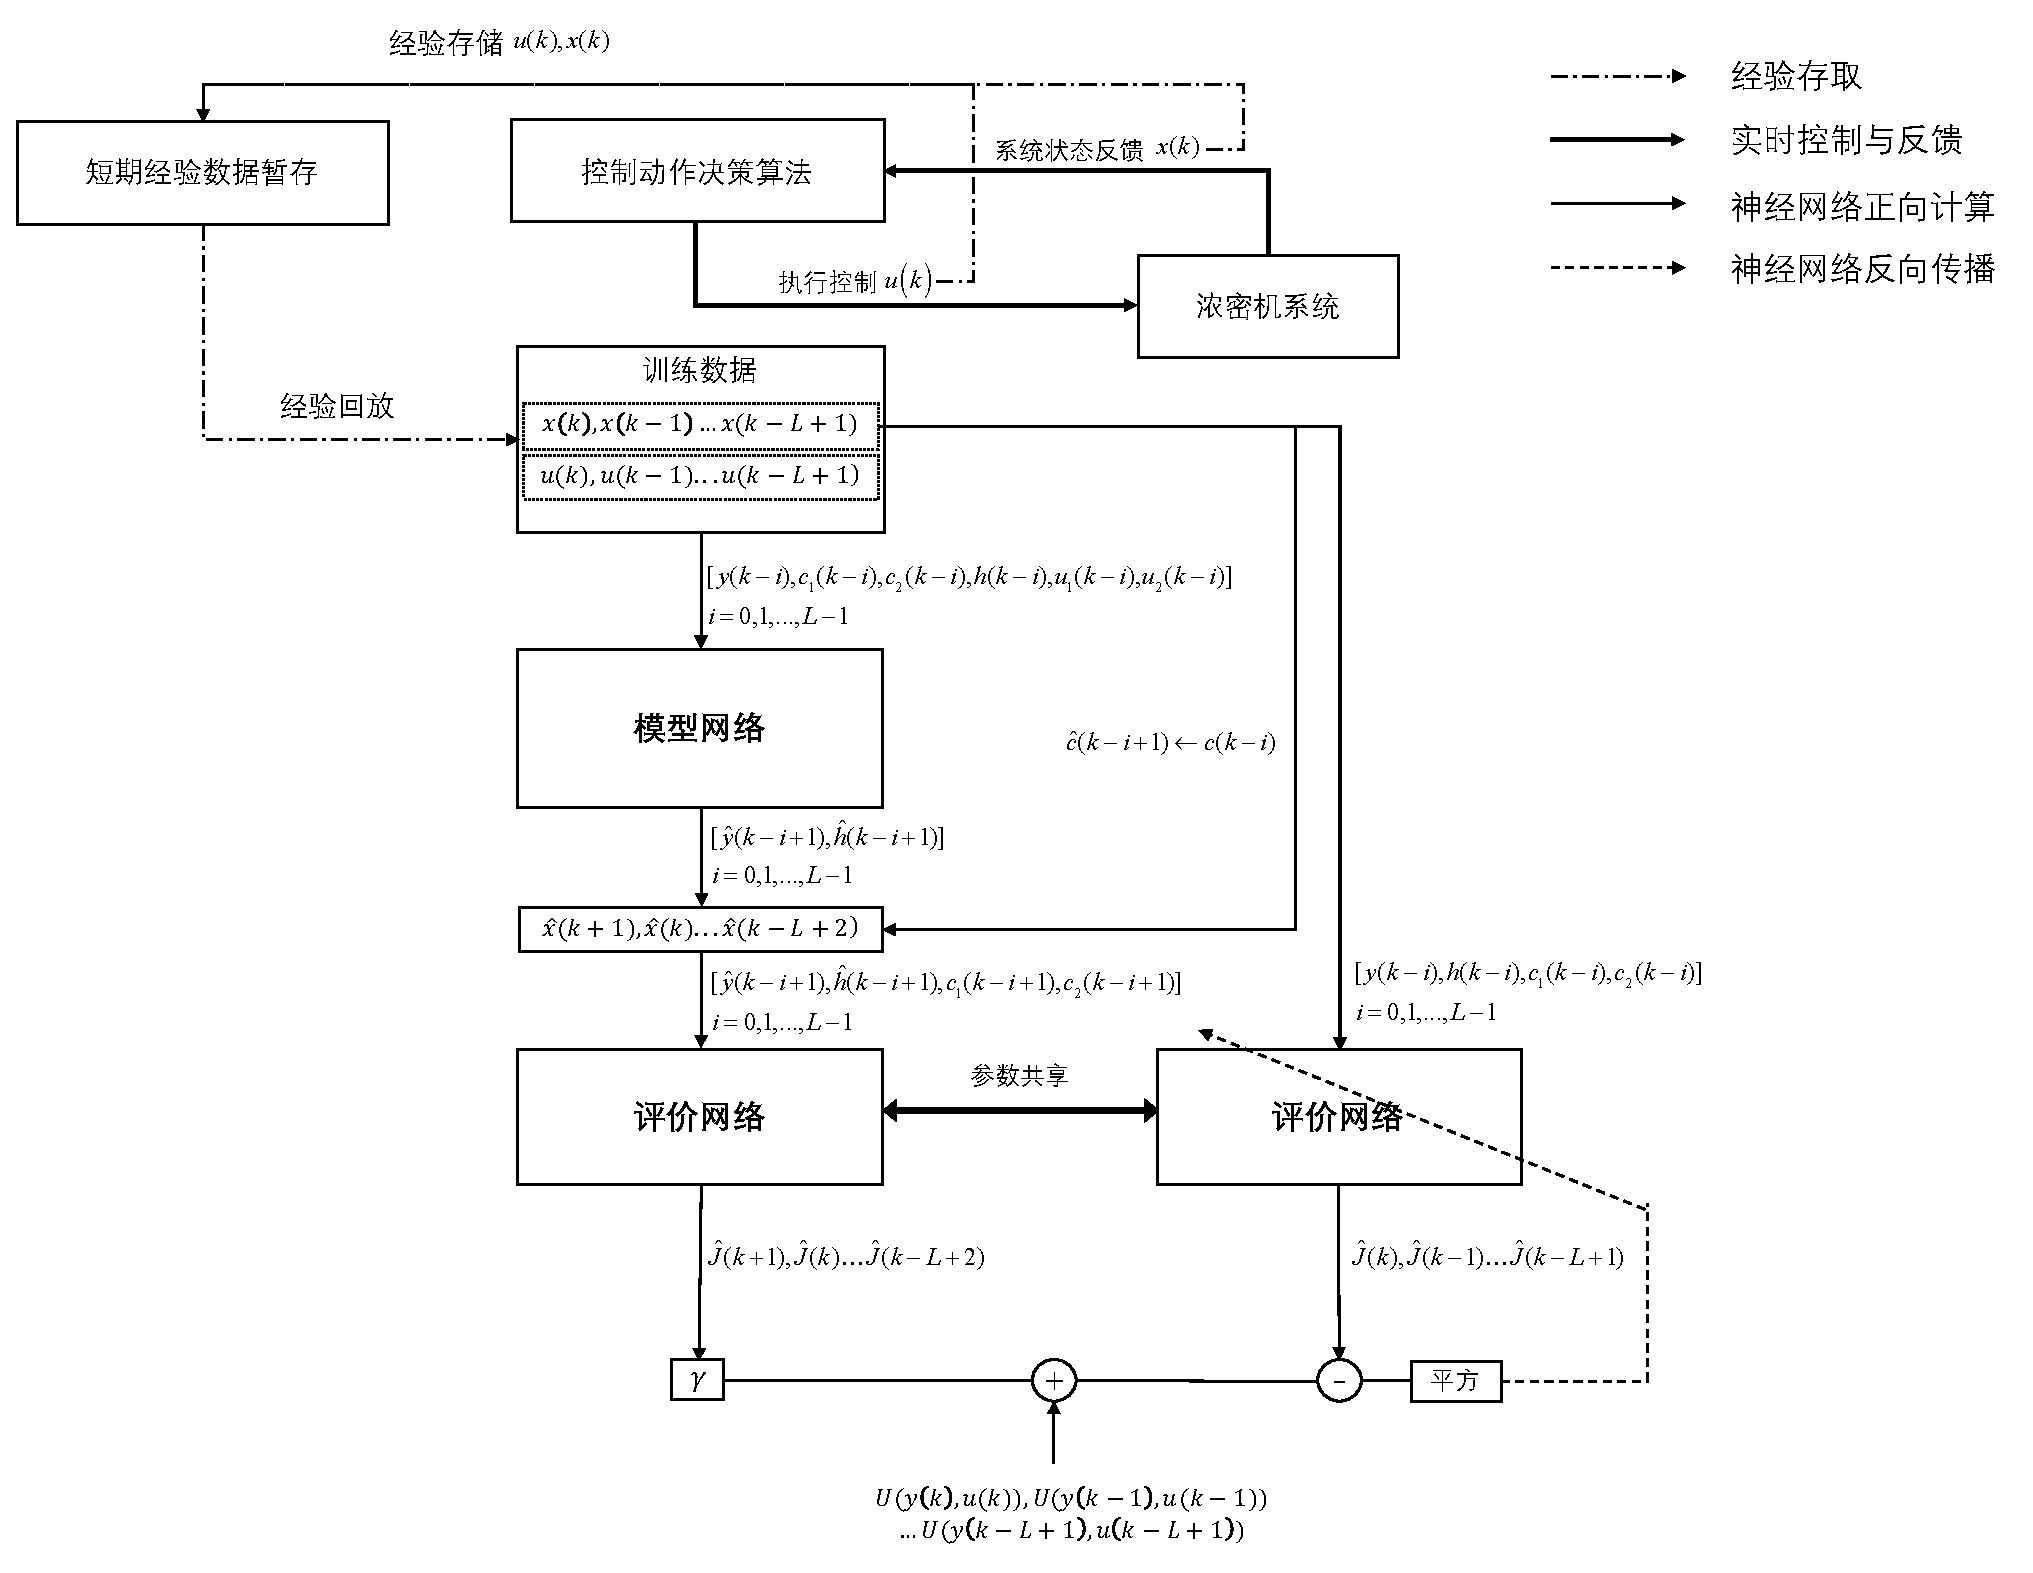
\includegraphics[width=17cm]{figures/chapter6/fig2.eps}
%     \caption{HCNVI算法结构示意图}

% %%%%%%%%%%%%%英文标题begin
%   \addtocounter{figure}{-1}
%   \vspace{-5pt}
%   %\SetEnglishCaption
%   \renewcommand{\figurename}{Fig.}
%   \caption{Structure diagram of algorithm HCNVI}
%   \renewcommand{\figurename}{图}
% %%%%%%%%%%%%%英文标题end
%     \label{fig:alg_structure}
% \end{figure*}
% \subsection{基于ODE-Net的系统预测网络}
% 建立模型网络用来对系统动态进行建模,根据当前系统状态、外部噪音量、控制输入、预测下一时刻底流浓度和泥层高度变化。网络结构仍采用单隐层神经网络,如图\ref{fig:nn_structure}所示。模型网络具体定义如下:
% \begin{equation}
% \label{modelNN} [\hat{y}(k+1), \hat{h}(k+1)]^{\rm T}=W_{m 2} \tanh
% \left(W_{m 1}( \b \phi(k))\right)
% \end{equation}
% 其中$\b \phi (k)=[\b x(k)^{\rm T}, \b u(k)^{\rm T}]^{\rm T}$,\\
% 网络输入层包含6个节点,隐层包含20个节点,输出层2个节点,$ W _ { m1
% }$和$ W _ { m 2 }$内各个参数均初始化为$-1\sim 1$之间的随机数。
% 通过梯度下降方法训练模型网络:
% \begin{equation}
% \label{equ:train_modelnn} W_{mi}(k)=W_{m i}(k)-l_{m } \frac{\partial
% E_{m}(k)}{\partial W_{m i}(k)}
% \end{equation}
% 损失函数$E_{m}(k)$定义为:
% \begin{equation}
% \label{equ:loss_modelnn} E_{m}(k)=\frac{1}{2} \b e_{m}^{\rm
% T}(k)\b L_{m}\b e_{m}(k)
% \end{equation}
% \begin{equation}
% \label{em_modelnn}
% \begin{aligned} e_{m}(k)&=[\hat{y}(k+1), \hat{h}(k+1)]^{\mathrm{T}}-\\ &[y(k+1),h(k+1)]^{\mathrm{T}} \end{aligned}
% \end{equation}
% %e_{m}(k) = \left[[\hat{y}(k+1),\hat{h}(k+1)]^{\mathrm{T}}- \\ [y(k), h(k)]^{\mathrm{T}}\right]
% 对于模型网络,同样采用\equref{equ:normalize}对训练数据进行放缩。
% 模型网络的训练全部离线进行,在控制任务开始后,将不再对模型网络进行调整。
\subsection{基于积分强化学习的策略评价}
% 连续时间自适应动态规划算法
% \label{sec:ctirl}
% qqq
% qqq
% qqq
% qqq
% qqq
% qqq
% \vspace{-50pt}
本节采用积分强化学习算法\cite{Guo2019}训练策略评价模型。
对\equref{equ:goal}中定义的折扣积分奖赏,可以表示为贝尔曼方程的形式:
% 求解理想情况下最优控制输入$\b u^*(k)$。
\begin{equation}
  \hat{V}^{H}\left(\mathbf{s}_{0}\right)=\int_{0}^{H} e^{-\frac{\tau}{\eta}} U(\hat{\mathbf{s}}(\tau), \hat{\mathbf{a}}(\tau)) d \tau+e^{-\frac{H}{\eta}} {V}\left(\hat{\mathbf{s}}_{H}\right)
  \label{equ:J_bellman}
\end{equation}
其中$H$为任一积分范围,$\b s_H$ 为$H$时刻的终止状态。根据贝尔曼最优原则,$\b s_0$所在时刻的最优评价值函数$V^*(s_0)$满足连续哈密顿-雅可比-贝尔曼方程:
\begin{equation}
\label{equ:J_star} 
V ^ { * } \left( s_0 \right) = \min _{ \mathbf u[0:H ] } \{ \int_0^H e^{-\frac{\tau}{\eta}} U(\hat{\mathbf{s}}(\tau), \hat{\mathbf{u}}(\tau)) d\tau  + e^{-\frac{H}{\eta}} \hat{V}^*\left(\hat{\mathbf{s}}_{H}\right)\}
\end{equation}
对于任意范围$[0:H]$,最优的控制输入$\b u^*[0:H]$可以表示为:
\begin{equation}
\b u^*[  0:H ] =\arg \min _ { \b u[0:H ] }\{ \int_0^H e^{-\frac{\tau}{\eta}} U(\hat{\mathbf{s}}(\tau), \hat{\mathbf{u}}(\tau))  + e^{-\frac{H}{\eta}} \hat{V}^*\left(\hat{\mathbf{s}}_{H}\right)\}
\label{equ:VI_u}
\end{equation}
% 由于\equref{equ:system_dynamic}中$f(\cdot)$是未知的,因此可以采用值迭代算法寻找最优控制策略,定义
% ,$\Omega _ u = \{u:u _ { \text {  min } } \leq u \leq u _ { \text {
%     max } }\}$,$x[k]=[y(k),  h(k),c ( k )^{\rm T} ]^{\rm T}$

% 由于\equref{equ:system_dynamic}中$f(\cdot)$是复杂非线性函数,无法直接对\equref{equ:J_star}进行求解,但可以利用算法\ref{alg:VI}以值函数迭代的方式求解最优值函数和最优控制律,其中$\b s(t_k)$用于表征$t_k$时刻的系统状态。根据文献\cite{Wang2012-GDHP},可以证明当$i\rightarrow
% \infty$时,值函数$V _ { i } \rightarrow V ^ { * }$,控制律$\b u _
% { i } \rightarrow \b u ^ { * }$。
% \begin{algorithm}[hpbt]

% \caption{值迭代算法} %算法的名字
% \label{alg:VI}
% \hspace*{0.02in} {\bf 初始化:} %算法的输入, \hspace*{0.02in}用来控制位置,同时利用 \\ 进行换行
% 随机定义 $V_0(\cdot)$
% \begin{algorithmic}[1]
% \State 定义控制约束集合$\Omega _ {\b u} = \{\b u:\b u _ {
% \text {  min } } \leq \b u \leq \b u _ { \text {     max } }\}$
% \For{$i=0,1,2,...,\infty$} % For 语句,需要和EndFor对应
% % \State 根据当前值函数 $V_i(\cdot)$寻找最优控制策略
% \State 策略改进
% \begin{flalign}
%     \label{equ:VI_u}
%         & \b u _ { i } \left( t \right) = \arg\min_{\b u(t)}\in \Omega_{\b u} U(y(t),\b u(t)) + \gamma V _ { i } (\b s(t))
% \end{flalign}
%   \State 策略评估
% \begin{flalign}
% \label{equ:VI_v}         V _ { i + 1 } \left( \b x(k) \right)
% = U(y(k),\b u_i(k)) + \gamma V _ { i } (\b x(k+1))
% \end{flalign}
% \EndFor

% \end{algorithmic}
% \end{algorithm}

% \subsection{基于积分强化学习的连续时间Actor-Critic算法}

原则上,利用\equref{equ:VI_u}即可获得最优控制策略。\equref{equ:VI_u}等号右侧的第一项为积分奖赏项,
% 类似于\eqref{equ:state_traj},利用训练得到的ODE-Net对产生的系统轨迹进行奖赏积分评估即可求得。
可以通过\eqref{equ:state_traj}预测系统轨迹,并在求解轨迹上同时对效用函数进行积分以近似$[0:H]$之间的控制代价。
第二项为无穷积分项,无法显式求解。因此本章引入值函数近似的方法以评估未来的积分奖赏项。
具体地,HCNVI构建评价网络$V_\xi(\cdot)$近似给定策略的评价函数:
\begin{equation}
\label{equ:criticNN} \hat { V }_\xi ( \b s(t) ) = W _ { c 2 } \tanh \left( W _
{ c 1 }  \b s(t)  \right)
\end{equation}
$\tanh(s)=\frac{\rm e^{s}-\rm e^{-s}}{\rm e^{s}+\rm
e^{-s}}$是网络的激活函数,网络输入层包含$n+l+d$个节点,输出层1个节点。网络参数
% $\xi=[W _ { c 1 }, W _ { c 2 }]$内参数均初始化为$-1\sim 1$之间的随机数。
为了保证算法参数更新的实时性,采用系统在线控制过程中产生的增量数据训练网络。
具体地,采用单步时序差分误差(Temporal difference error,TD error)\cite{Sutton2018}计算评价网络的估计误差值。
假设从被控系统中采集的相邻数据点为$\{\b s(t_k), \b u(t_k)\},\{\b s(t_{k+1}), \b u(t_{k+1})\}$,
% 见\equref{equ:TDerror}。值估计$\hat{V}_\xi(\cdot)$ 近似于有限区间奖赏积分与未来奖赏的和,且都任意积分区间均成立,因此本章计算积分区间长度边缘分布下时序差分误差的期望:
时序差分误差计算过程如\equref{equ:TDerror}所示:
\begin{equation}
\label{equ:TDerror} e_{c }(\b s(t_k))=\hat{V}_{\xi}(t_k)-e^{-\frac{\Delta t}{\eta}} \hat{V}_{\xi}(t_{k+1})+\int_{t_k}^{t_{k+1}}e^{-\frac{\tau-t_k}{\eta}}U(\b s(\tau), u(\tau))d \tau
\end{equation}
其中$\Delta t=t_{k+1}-t_{k}$,
$\hat{V}_{\xi}(t_k)=\hat{V}_{\xi}(\b s(t_k))$,
网络损失函数为$E_c(t_k)=e_c^2(\b s(t_k))$。通过极小化该目标函数,可以使评价网络根据被控系统的状态信号及效用值信号,实时地、增量式地逼近对于当前控制策略的评价函数。
使用链式法则可以计算损失值$E_c(t_k)$对网络参数的梯度:
\begin{equation}
\begin{aligned}
\label{equ:critic_gradient} \dfrac{\partial e_c^2(\b s(t_k))}{\partial
W_{c2}} & =2e_c(\b s(t_k)) \tanh(W_{c1}\b s(t_k))^{\rm T} 
\\ \dfrac{\partial
e_c^2(\b s(t_k))}{\partial W_{c1}} & =2e_c(\b s(t_k)) [W_{c2}^{\rm
T}\odot(1-\tanh^2(W_{c1}\b s(t_k)))]\b \b s(t_k)^{\rm T}
\end{aligned}
\end{equation}

采用梯度下降算法对评价网络进行训练更新:
\begin{equation}
\label{equ:train_critic} W_{ci}(t_k)=W_{ci}(t_k)-l_{c} \frac{\partial
e_{c }^{2}(t_k)}{\partial W_{ci}(t_k)}\text{, }i=1,2
\end{equation}

其中$l_c$是学习率。由于一般工业系统所处环境的外界噪音是不断波动的,当外界噪音$\b
c(t)$改变时,网络需要利用实时采集的数据快速收敛到新的参数,因此$l_c$需设定为固定值以保持在线学习能力。

由于不同物理量的取值差异很大,会导致网络无法有效学习并且造成超参数设定困难。因此本章采用系统产生的离线数据中各参量的极值对所有训练数据进行归一化放缩。
\begin{equation}
\label{equ:normalize} \overline{z}=\frac{2\left(z-z_{\min
}\right)}{z_{\max }-z_{\min }}-1
\end{equation}
%%%%%%%%%%%%%%%%%%%%%%%%%%%%%%%%%%%%%%%%%%%%%%%%%%%% 正文2.3

\subsection{基于随机梯度下降的动作生成}
大部分的自适应动态规划算法,如HDP、DHP\cite{Werbos2008}等都通过建立动作网络计算控制输入,并利用评价网络输出值训练动作网络的参数。
在本章提出的HCNVI方法中,以随机梯度下降的方式取代了动作网络,直接利用评价网络和ODE-Net模型计算控制动作。
该方法可以在环境噪音改变时,及时更新控制策略,使被控系统更快速地收敛到理想状态。同时能够减少内存占用并省去训练动作网络的时间开销。

给定系统状态$\b s(t_k)$下,利用评价网络和模型网络计算控制动作${\b
u}(t_k)$的过程如算法\ref{alg:find_optimal_policy}所示。
\equref{equ:estimate_J_next}中在估计$t_{k}+h$时刻的折扣累计惩罚时,下一时刻系统所处外界噪音是未知的。不过由于真实工业环境下进料噪音都是连续变化的,很少出现突变,因此本模型采用当前时刻噪音$\b
c(t_k)$充当未来一段时间的外部噪音$\b c[t_k:t_k+h]$。

\begin{algorithm}[htb]
\caption{利用迭代梯度下降算法计算控制动作} %算法的名字
\label{alg:find_optimal_policy}
\hspace*{0.02in} {\bf 输入:} %算法的输入, \hspace*{0.02in}用来控制位置,同时利用 \\ 进行换行
第$t_k$时刻系统状态$\b s(t_k)=[\b y(t_k),\b h(t_k),\b c(t_k)]$\\
\hspace*{0.02in} {\bf 输出:} %算法的输入, \hspace*{0.02in}用来控制位置,同时利用 \\ 进行换行
第$t_k$时刻的控制动作输出${\b u}(t_k)$
\begin{algorithmic}[1]
\State 随机选取$
\begin{array}{c}{\b u_{0}=\left[v_{1}, v_{2}\right]^{\rm T}} \end{array}
$,其中 $v_{1} \sim U(-1,1) , v_{2} \sim U(-1,1)$ 
\State $c=0$
  \Do
    \State 随机采样$M$个时间点$0 < h_1, \cdots, h_M \leq H$。
    \For{$\b h_i\in\{h_1, \cdots, h_M\}$}
    % \State 均匀采样$\b h\in \mathbb{R}^M,\quad h_i \sim \mathcal{U}(0,H)$给定$\b u[t:t+H]=\b u _i$下,预测$[t,t+h]$范围内的奖效用函数积分及:
    \State 评估积分区间为$[t_k,t_k+h_i]$下,$t_k$时刻的评价值$\hat{V}(\b s(t_k))_i$。
    \begin{equation}
    \hat{V}(\b s(t_k))_i = \int_{t_k}^{t_k+h_i}e^{-\frac{\tau-t_k}{\eta}}U(\hat{\b s}(\tau),{\b u}(\tau))d\tau+e^{-\frac{h_i}{\eta}}\hat{V}_\xi(\b s(t_k+h_i)) 
    \label{equ:estimate_J_next}
    \end{equation}
    其中$\hat{\b s}(\tau)$为模型网络给出的预测轨迹,$\b u(\tau)=\b u _c$
%     \State 令$\hat{\b x}(k+1)=[\hat{y}(k+1), \hat{h}(k+1),\b c(k)^{\rm T}]^{\rm T}$,估计$k+1$时刻评价值
%     \begin{equation}
% \hat{J}(k+1)=W_{c 2} \tanh \left(W_{c 1}(\hat{\b x}(k+1))\right)
%     \end{equation}
% \State 计算第$k$时刻评价值
% \begin{equation}
%   \label{equ:estimate_J_in_k}
%     \hat{J}(k)=U\left(y_{k}, \b u_{i}\right)+\gamma \hat{J}(k+1)
% \end{equation}
\EndFor
\State 求取$M$轮采样下评价值的均值,并利用梯度下降算法对$\b u_c$进行更新
\begin{equation}
\b u_{c+1}=\b u_c- \frac{l_u}{M}\sum_{i=1}^{M}\frac{\partial \hat{V}(\b s(t_k))_i}{\partial \b u_{c}}
\end{equation}
\State 将$\b u_{c+1}$限定在控制约束内
\begin{equation}
\b u_{c+1} = \max([-1,-1]^{\rm T}, \min([1,1]^{\rm T},\b u_{c+1}))
\end{equation}
\State $c=c+1$
  \doWhile{$\left\|\b u_{c}-\b u_{c-1}\right\|>\epsilon_{a}$} and $c<Na$ % <--- use \doWhile
  \State 反归一化,并求得${\b u}(t_k)$
 \begin{equation}
\b u(t_k)=\frac{\b u_{c} \odot\left(\b u_{\max }-\b u_{\min
}\right)}{2}+\b u_{mid }
\end{equation}
\State return $\b u(t_k)$
\end{algorithmic}

\end{algorithm}

为了验证算法\ref{alg:find_optimal_policy}的有效性,本章对\equref{equ:estimate_J_next}算得的$\mathbb{E}[\hat{V}(t_k)]$与${\b u}(t_k)$的关系及迭代求解$\b u({t_k})$的过程进行了可视化探究。
在实验一\ref{sec:vi_hdp_stable}介绍的仿真实验中挑选了三个时刻分析了$\mathbb{E}[\hat{V}(t_k)]$与${\b u}(k)$之间的函数关系。
图\ref{fig:J_u_cmp}中的三个子图分别代表训练开始阶段、第一次系统达到稳态时、第二次系统达到稳态时的可视化结果。
横纵坐标代表被归一化后的二维控制量,颜色深浅代表$\mathbb{E}[\hat{V}(t_k)]$的大小。黄色箭头线代表利用算法\ref{alg:find_optimal_policy}寻找最优控制输入${\b
u}(t_k)$的梯度下降轨迹。
根据实验结果发现:在网络训练的三个阶段中,图中颜色最深的点,即$\mathbb{E}[\hat{V}(t_k)]$的最小位置是唯一的,且不存在其他局部最优解。黄色箭头线能够准确地收敛至全局最优解。该结果说明由于最大积分长度$H$较小,同时工业系统运行过程满足利普希茨连续特性且,某一时刻的控制输入${\b
u}(t_k)$对下一时刻系统状态$\b
s(t_k+h_i)$影响相对较小,且评价网络\equref{equ:criticNN}和效用函数\equref{equ:U}具有连续、可微的性质,因此$\mathbb{E}[\hat{V}(t_k)]$随${\b
u}(t_k)$变化的分布函数在给定的控制约束下一般为单峰函数。
采用梯度下降算法可以有效地寻找到全局最优的$\b u^*(t_k)$,而不会收敛到局部最优解,进而满足\equref{equ:VI_u}的最小化条件,实现最优控制。

%另外,本章通过对$U(k)+\gamma
%J(k+1)$与${\b u}(k)$的关系进行可视化,发现由于浓密机运行过程缓慢,某一时刻的控制输入${\b u}(k)$对下一时刻浓密机状态$x(k+1)$对影响相对较小,同时利用神经网络构建的评价网络\equref{equ:criticNN}和效用函数\equref{equ:U}具有连续、可微的性质,$\hat{J}(k)$随${\b u}(k)$变化的分布函数一般情况下为单峰函数,因此采用梯度下降算法可以比较有效地寻找到全局最优的$u^*(k)$,而不会收敛到局部最优解。
\begin{figure*}[htb]
    \centering
    %fig 1
    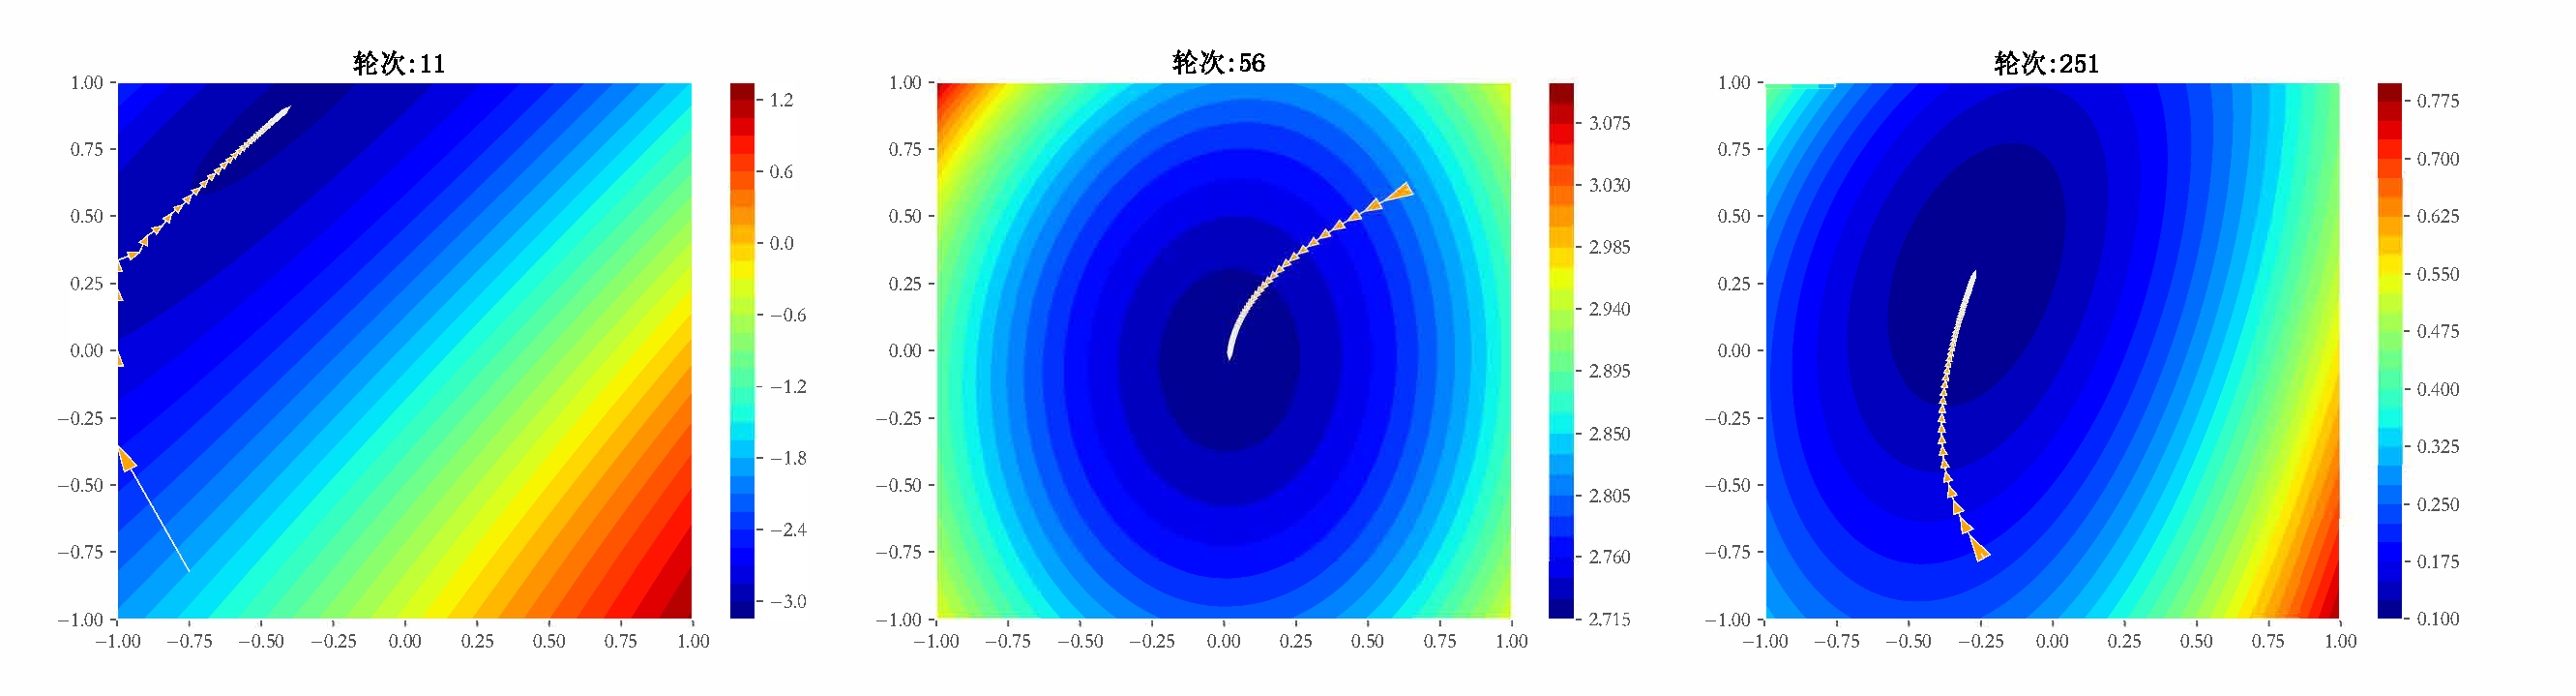
\includegraphics[width=\linewidth]{figures/chapter6/fig4.pdf}
    \caption{迭代梯度下降过程可视化}
    %\\
  % \caption{ Fig. Visualization of the relation between ${\b u}(k)$ and $U(k)+ \gamma J(k+1)$}
\label{fig:J_u_cmp}
\end{figure*}
\subsection{短期经验回放}
为了增加评价网络训练的准确性和收敛速度,本章进一步提出短期经验回放方法优化网络训练的损失函数,以达到优化局部评价值梯度准确性的目的。
短期经验回放方法创建经验回访池存储$L$步内的状态-动作轨迹$\{(\b s(t_k), \b u(t_k))\text{,}$$\cdots \text{,}$$\b s(t_{k+L}), \b u(t_{k+L})\}$,在训练过程中,短期轨迹数据可以用于共同计算评价网络的损失值以及优化梯度方向。
在当前时刻$t_{k+L}$,\equref{equ:TDerror}的误差值计算方法修改为:
% \begin{equation}
%  e_{c}(k)=\frac{1}{L} \sum_{i=0}^{L-1}
% \hat{J}(\b x(k-i)) - (U(k-i)+\gamma \hat{J}(\b x(k-i+1)))
% \end{equation}
\begin{equation}
  e_{c }(t_{k+L})=\frac{1}{L}\sum_{i=0}^{L-1}[\hat{V}_{\xi}(t_{k+i})-e^{-\frac{\Delta t_i}{\eta}} \hat{V}_{\xi}(t_{k+i+1})-\int_{t_{k+i}}^{t_{k+i+1}}e^{-\frac{\tau-t_{k+i}}{\eta}}U(\b s(\tau), u(\tau))d \tau]
  \label{equ:TDerror_replay}
  \end{equation}
  其中 $\Delta t_i = t_{k+i+1}-t_{k+i}$。
% 通过存储短期内被控系统的运行轨迹数据,
诸如HDP、DHP以及本章提出的HCNVI算法都是面向状态值函数进行建模的在线控制算法,其策略模块的更新都是以模型网络作为媒介,计算评价网络输出值$\hat{V}(t_k)$对于控制输入${\b
u}(t_k)$的梯度,并在此梯度基础上更新动作网络或者利用算法\ref{alg:find_optimal_policy}优化${\b u}(t_k)$。
因此对于${\b u}(t_k)$梯度估计的准确性极大地影响了策略模块的更新效果,进而影响整个控制系统的控制效果与收敛速度。${\b u}(t_k)$的梯度表达式为\equref{equ:uk_grad}
\begin{equation}
\label{equ:uk_grad} \nabla \b u(t_k)=\gamma\frac{\partial \b s(t_{k+1})}{\partial \b u(t_k)}\frac{\partial\hat{V}(t_{k+1})}{\partial \b s(t_{k+1})}+\frac{\partial U(t_k)}{\partial \b u(t_k)}
\end{equation}
式中的$\frac{\partial\hat{V}(t_{k+1})}{\partial \b
s(t_{k+1})}$也称为$t_{k+1}$时刻的协状态$\lambda(t_{k+1})$,代表了评价网络输出值对于系统状态量的梯度。模型网络可以利用系统离线数据进行训练,在训练数据量充足时可以达到极高的精度,可以近似认为$\frac{\partial
\b s(t_{k+1})}{\partial \b u(t_k)}$的估计是足够精确的。
$U(t_k)$作为确定的效用函数使得$\frac{\partial U(t_k)}{\partial \b
u(t_k)}$是准确的。因此对于$\nabla \b
u(t_k)$的估计误差主要来源于对协状态$\lambda(t_{k+1})$的估计误差。

对于大部分的大型过程工业设备,系统的运行过程缓慢,短时间内系统状态不会发生剧烈改变,即$\b s(t_k)\approx \b s(t_{k+1})$,且评价网络具有连续可微的性质。因此可以近似认为$\lambda(t_k)\approx \lambda(t_{k+1})$。
同样,由于系统运行过程缓慢会导致提供给控制模型学习的训练数据中系统状态参量分布非常集中,可以近似认为\equref{equ:x_equation}成立。
\begin{equation}
\label{equ:x_equation} \forall 1 \leq i<L, \| \b s(t_{k-i})-\b s(t_i)||<\delta
\end{equation}
该式表明短期内系统状态点$\b s(t_{k-i})$都在以$\b s(k)$为中心,$\delta$为半径的邻域内。
通过\equref{equ:TDerror_replay}将短期$L$条数据共同用于评价网络训练,可以使评价网络在$\b s(t_k)$的邻域内学习地更佳充分,进而更准确地估计$\lambda(t_k)$。

% 对于HDP、DHP等面向状态值函数进行建模的在线控制算法来说,根据被控系统的运行轨迹数据训练控制模型,
% 其模型收敛过程和被控系统达到稳定的过程是同步的。被控系统在控制模型的控制作用下,在状态空间内不断游历,每一次系统状态改变所产生的轨迹数据将使控制模型产生参数上的更新,控制模型参数的更新又会影响此刻控制输入的计算,进而影响被控系统未来的状态轨迹。

% 控制策略产生控制动作的过程,本质上就是对评价网络输出的评价值进行梯度反向传播,然后让策略模块去学习输出驱使系统状态中的各个分量向其梯度下降的方向迁移的控制动作,
% 促使被控系统进入一个评价值更低的状态。当系统状态进入了一个局部最小评价值点,则控制模型收敛。
% 如果该点是全局评价值最小点,在参数$Q,R$的设定值相对适宜的情况下,则实现了该系统的最优控制,被控系统也进入稳定状态。

% 对于浓密机等大型流程工业设备来说,系统的运行过程缓慢,短时间内系统状态不会发生剧烈改变,即$x(k-1)\approx
% x(k)\approx
% x(k+1)$,这就导致了向控制模型输入的训练数据中系统状态参量分布非常集中,评价函数几乎不能通过在线训练得到全局分布均匀的训练数据,也就无法满足全局评价值估计的准确性,只能满足局部评价值估计的准确性,即在$x(k)$附近的评价值估计是相对准确的。而想要通过局部评价值准确性来引导控制器输出对被控系统有益的控制动作
% \begin{equation}
%     \label{equ:Vcompare}
%     J^*(k+1)<J^*(k),x(k+1)=f(x(k),u(k))
% \end{equation}
% %图\ref{fig:J_u_cmp} 图\ref{fig:replay_compare}
% %图\ref{fig:no_replay} 图\ref{fig:stable_noise_input}
% 其关键在于,值函数网络输出值$J(x(k))$对$x(k)$的梯度,也被称为协状态的准确性。通过\equref{equ:TDerror_replay}将短期数据共同用于评价网络训练,可以防止网络输出值整体飘逸,在系统当前所处状态空间的局部邻域内,评价网络能够正确评估局部梯度方向,有效地对输出的控制动作进行校准。
\begin{figure*}[!tbp]
\centering 
\subfigure[无经验回放.] {
  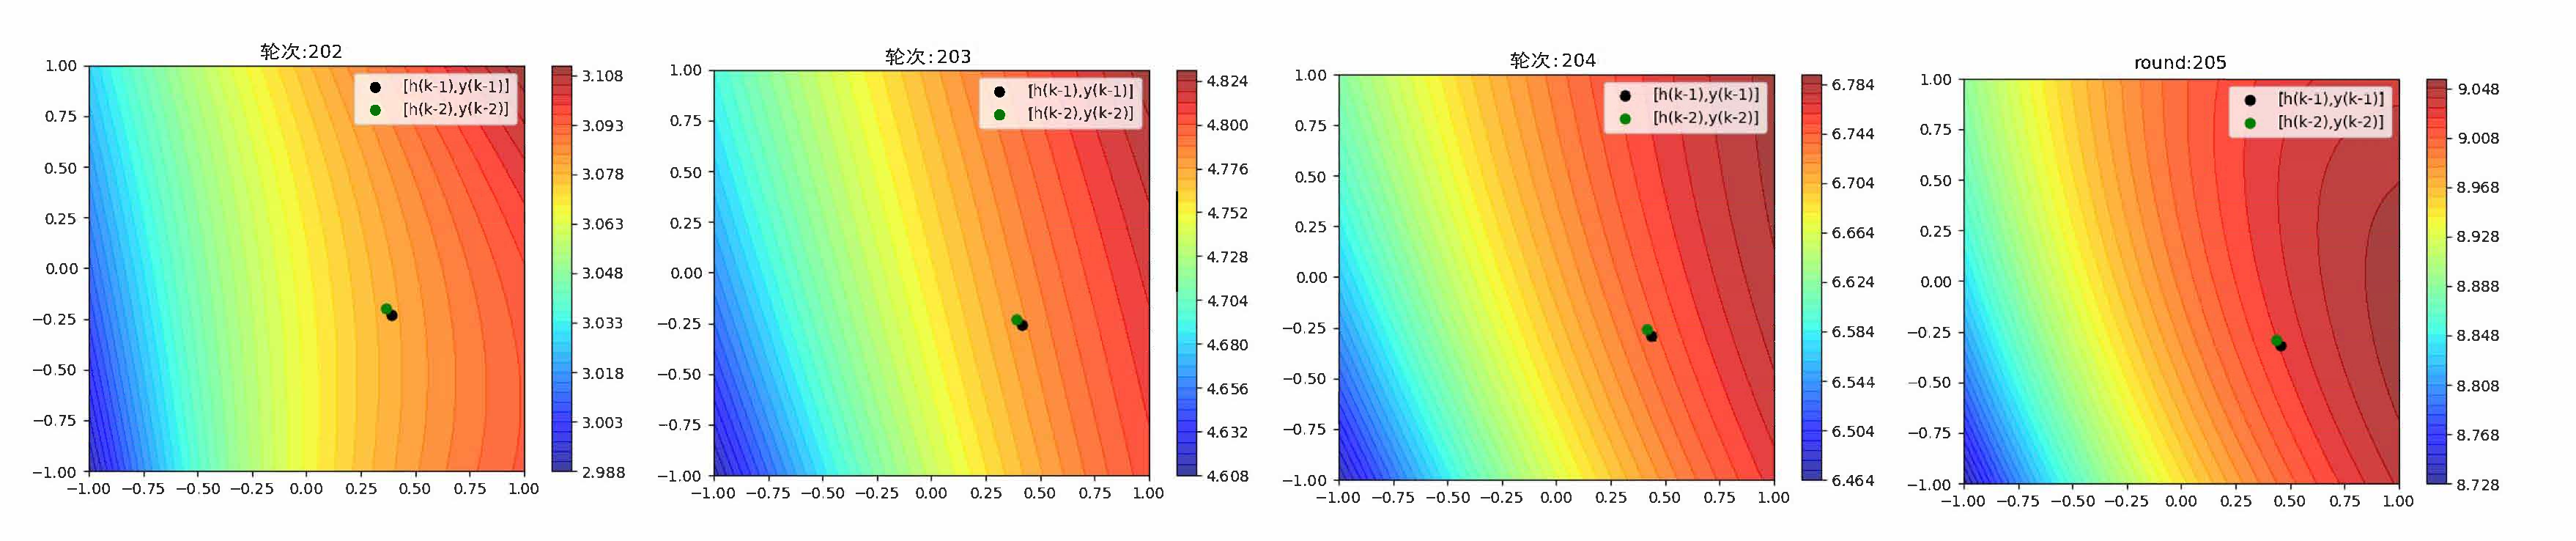
\includegraphics[width=\linewidth]{figures/chapter6/fig5a.eps}
  \label{fig:6_no_replay}
  }
\subfigure[经验回放点数量为2.]
{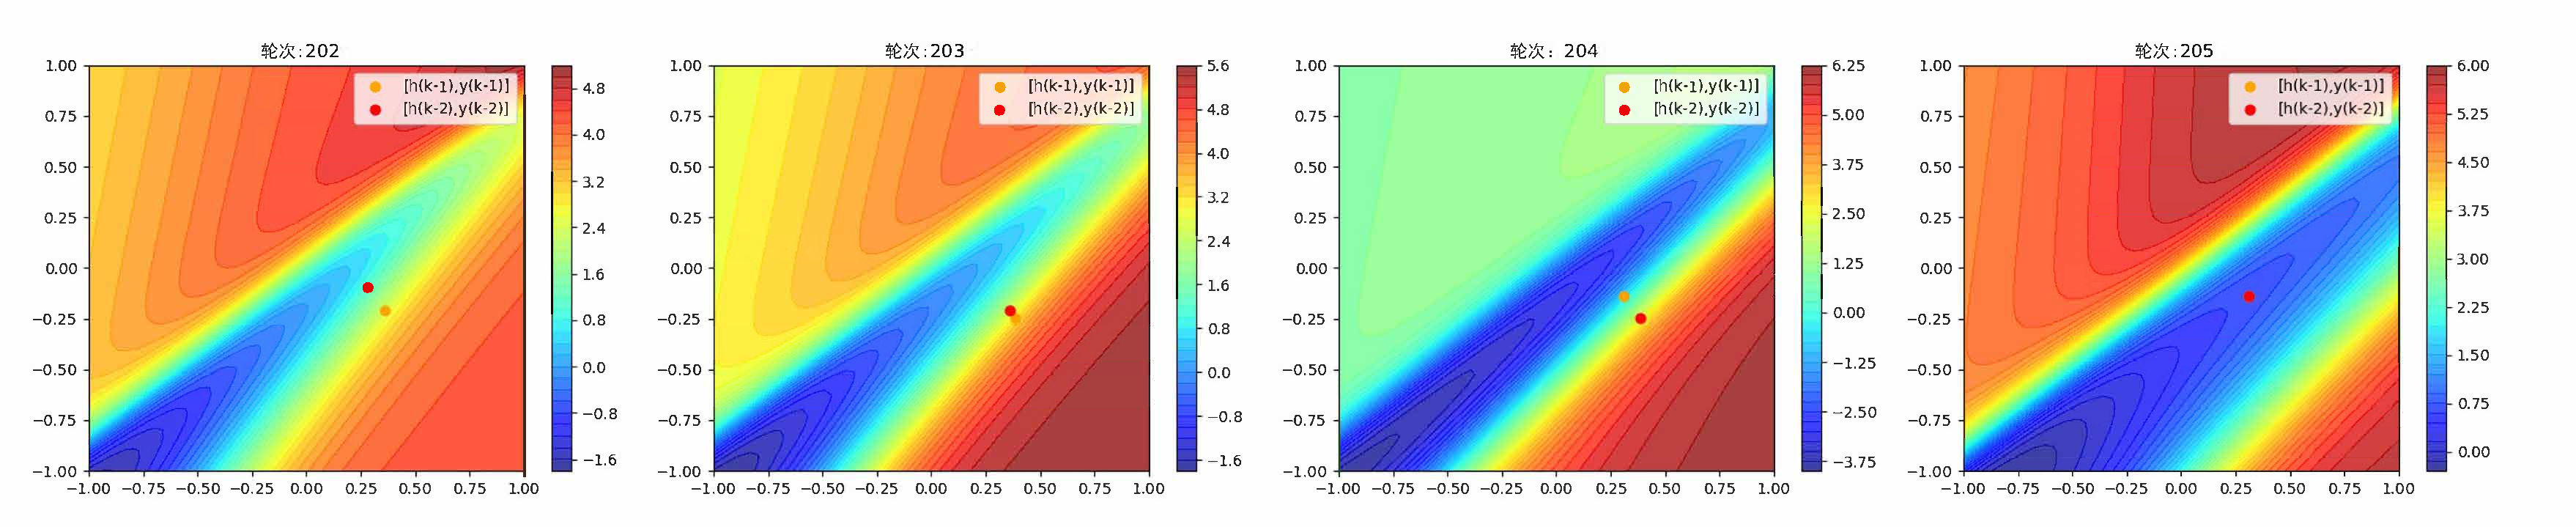
\includegraphics[width=\linewidth]{figures/chapter6/fig5b.eps}}
\caption{短期经验回放对评价网络的输出值的影响 }
\label{fig:replay_compare}
\end{figure*}
为了更直观地展示增加短期经验回放对评价网络学习过程的影响
,本章对实验一\ref{sec:vi_hdp_stable}节中的评价网络进行了可视化,实验结果如图\ref{fig:replay_compare}所示。该实验中采用等高线图对评价网络的输出值进行展示,其中图\ref{fig:replay_compare}(a)代表不使用经验回放,利用\equref{equ:TDerror}训练网络,图\ref{fig:replay_compare}(b)代表使用短期经验回放,回放数据点数$L$为2,利用\equref{equ:TDerror_replay}训练网络。对于两种算法,分别绘制了连续四次迭代中,评价网络在更新后对不同泥层高度$h(\cdot)$和底流浓度$y(\cdot)$的评价值。
图中横纵坐标分别代表被归一化后的泥层高度和底流浓度。
根据实验结果发现。在图\ref{fig:replay_compare}(a)中评价网络的输出值在不同输入下基本趋同。且在当前时刻系统状态点附近,网络输出值的梯度很小。
说明单数据点更新会造成评价网络很快地遗忘历史数据,导致网络输出值整体漂移,难以稳定地学习到正确的局部梯度。在图\ref{fig:replay_compare}(b)中,当前系统状态($h(t_k)$,$y(t_k)$)所处邻域内,网络输出值具有较大差异,局部梯度值可以被较好地保持。
准确的梯度$\lambda(t_k)$可以提高$\nabla \b
u(t_k)$估计的精确度,因此对短期数据进行回放训练可以更好地指导控制策略输出更优控制动作,促使评价网络和被控系统快速收敛。
同时,当经验回放数据量\equref{equ:TDerror_replay}中$L$的过大,会导致性能的退化。其原因在于本章提出的方法是同策略(On-Policy)强化学习方法,而时间相差较远的历史数据点不能表征由当前控制策略产生的控制轨迹,因此评价网络会学习到错误的评价值。另外,$L$过大将不再满足性质\equref{equ:x_equation},过多的历史数据回放将不再有助于评价网络学习$\b
x(t_k)$处的梯度值$\lambda(t_k)$,进而不会提高对$\nabla \b
u(t_k)$估计的精确度。通过实验观察,一般将$L$限定在$5$以内,本章也将这种经验回放方法称为短期经验回放。



将HCNVI算法用于复杂工业系统在线控制的具体流程如算法\ref{alg:HCNVI}所示。

\begin{algorithm}[htb]

\caption{利用HCNVI算法实现复杂工业系统无模型在线控制} %算法的名字
\label{alg:HCNVI}

\begin{algorithmic}[1]

% \textbf{离线训练模型网络}
% \renewcommand{\algorithmicrequire}{\textbf{离线训练模型网络}}
% \renewcommand{\algorithmicrequire}{\textbf{在线浓密机控制}}

\State
使用系统运行离线数据,用\equref{alg:dyn}训练模型网络
\State $k=0$ \While{$k < T$}
\State 在新的采样时间点$t_k$获得系统观测值$y(t_k), h(t_k),\b c(t_k)$
% \If {$k\geq 1$} \State $i=0$ 
\Do
    \State 令$L=\min(L_c, k)$,用\equref{equ:TDerror_replay}求解$e_c(k)$
    \State 利用\equref{equ:train_critic}训练评价网络
    \State $i=i+1$
\doWhile{$i<N_c$ and $e_c(k)^2>\epsilon _c$}
% \While {$i<N_c$ or $e_c(k)^2<\epsilon _c$}
% \EndWhile
% \EndIf
%\State 利用\equref{equ:train_critic}训练评价网络,直到$e_c(k)^2<\epsilon$或

\State 利用算法\ref{alg:find_optimal_policy}求解${\b u}(k)$ \State
将${\b u}(t_k)$作用于被控系统,并等待下一次数据采样结果。 \State $k=k+1$

\EndWhile
\end{algorithmic}

\end{algorithm}

\section{仿真实验验证}
\label{sec:experiment}
接下来,本章将以工业浓密机系统为实验对象,探究HCNVI算法对于复杂工业系统的控制效果。浓密机系统的工作原理及相关参数介绍参见本文第三章实验部分。

底流浓度是浓密沉降控制过程的核心评价指标。
该因素受控制输入、系统状态参量、及其他外部噪音扰动影响。控制输入包括底流泵转速$u_1(k)$以及絮凝剂泵转速$u_2(k)$
,系统状态参量为泥层高度$h(k)$,外部噪音输入为进料流量$c_1(k)$、进料浓度$c_2(k)$。由于在部分工业场景中,上游工序产生的物料浓度、物料流量是不可控的,
% 。为了使提出的浓密机控制模型具有通用性,
因此本章将进料状态作为噪音输入量。浓密机进料颗粒大小,进料成分都会对浓密机底流浓度产生影响。不过由于此类变量无法观测且波动较小,为了简化问题,本章假定其保持恒定。
浓密机控制的首要目标是通过调节絮凝剂流量和底流流量使底流浓度$y(t)$追踪其设定值$y^*(t)$。另外,为了保证系统运行安全与仪器寿命,控制输入必须满足一定的限制条件。

当前大部分工业场景下,浓密机主要依靠操作员手工控制。操作员根据生产经验给出絮凝剂添加量的设定值($m^3/h$)以及底流流量设定值($m^3/h$),浓密机内相配套的回路控制系统会根据设定值的大小自动调节絮凝剂泵速($HZ$)与底流泵速($HZ$),使絮凝剂的实时流量、底流实时流量追踪操作员给出的设定值。
% 目前,在以PID控制为典型算法的回路控制技术领域已经有了较成熟的研究成果,在工业场景中获得了广泛应用。
% 因此在对浓密机的控制过程中,操作员给定的絮凝剂流量、底流流量目标值是否准确对于底流浓度能否满足要求有着至关重要的作用。
然而,由于浓密机系统具有较高的复杂性,操作员难以实时、完整地掌握系统运行参数,因此无法及时、准确地设定目标点位,最终导致浓密机在实际生产过程中时常处于非最优工作状态,底流浓度偏离理想设定值且频繁剧烈波动。
因此利用数据驱动算法实现浓密机系统的智能优化控制,能够有效降低操作员的作业难度及工作量,同时提升出料浓度的稳定性与控制精度。

\subsection{浓密机仿真模型}
% {\bf 浓密机仿真模型.}
% 由于
% 在浓密沉降控制过程的评价方面,其核心控制指标为底流浓度$y$ 。
% 对于浓密沉降控制过程的性能进行评价,其核心控制指标为底流浓度$y$ 。

% 根据上述定义,其中$\b u(t_k)=[u_1(t_k),u_2(t_k)] \in
% \mathbb{R}^2$为可控制输入量,$\b c(t_k)=[c_1(t_k),c_2(t_k)] \in
% \mathbb{R}^2$为不可控但是可观测的噪音量,$h(t_k) \in \bf
% R$为系统状态量,该参量是表征当前浓密机状态的重要参量,它可被间接控制但不作为控制目标
% 。因此,浓密机系统可表述为\equref{equ:system_dynamic}形式的非线性系统,其中$f
% ( \cdot )$为未知非线性函数。
% \begin{equation}\label{equ:system_dynamic}
%     [\dot y ( t_{k} ), \dot h(t_{k})]^{\rm T} = f (y(k), \b u ( k ) ,\b c ( k ) , h(k))
% \end{equation}

由于在真实工业场景下进行浓密机控制实验成本较高,不便于对不同控制算法的精度进行对比分析。因此本节首先采用浓密机仿真模型验证本章提出控制算法的有效性,下一节将介绍控制算法在真实工业浓密机系统上的控制效果。仿真模型构建方法参考了\cite{Chai2016, KIM2004403,WangLinyan2017,WangMeng,Tang2009,Wang330}。
该仿真模型建立在如下假设基础上:
\begin{itemize}
    \item 进料都是球形颗粒。
    \item  絮凝剂在浓密机的静态混合器中作用完全。
    \item 流体的扩散以固液混合物形式进行。
    \item 忽略颗粒间相互作用、浓密机中把机中轴的影响。
    %\item 忽略颗粒间相互作用、浓密机中把机中轴的影响、邝齿的运动和空间尺度。
\end{itemize}
模型推导过程中出现的变量如\tabref{tab:dynamic_variables},\tabref{tab:const_variable},\tabref{tab:variable_calculation}所示
% Please add the following required packages to your document preamble:
% \usepackage{booktabs}
% \usepackage{graphicx}
\begin{table}[htb]
\caption{参量定义} \label{tab:dynamic_variables}
\centering
%  %英文标题begin
%     \addtocounter{table}{-1}
%     \vspace{-0.2cm}
%     %\SetEnglishCaption
%     \renewcommand{\tablename}{Table}
%     \caption{Variables definition}
%     \renewcommand{\tablename}{表}
%     \vspace{0.4cm}
%  %英文标题end

\begin{tabular}{@{}lllll@{}}
\toprule
 变量                & 含义     & 量纲       & 初始值  & 补充说明 \\ \midrule
$f_{i}(t)$        & 进料泵频   & $Hz$     & 40   & 扰动量  \\
$f_{u}(t)$        & 底流泵频   & $Hz$     & 85   & 控制量  \\
$f_{f}(t)$        & 絮凝剂泵频  & $Hz$     & 40   & 控制量  \\
$c _ { i } ( t )$ & 进料浓度   & $kg/m^3$ & 73   & 扰动量  \\
$h(t)$            & 泥层高度 & $m$      & 1.48 & 状态量  \\
$c_u(t)$          & 底流浓度   & $kg/m^3$ & 680  & 目标量  \\
\bottomrule
\end{tabular}%
\end{table}

% Please add the following required packages to your document preamble:
% \usepackage{booktabs}
% Please add the following required packages to your document preamble:
% \usepackage{booktabs}
\begin{table}[htb]
  \centering
\caption{仿真模型常量}
\label{tab:const_variable}
% \resizebox{0.8\textwidth}{!}
% {
\begin{tabular}{cccc}
\toprule 变量            & 含义             & 量纲           &
参考值         \\ \midrule
$\rho _s$     & 干砂密度           & $kg/m^3$     & 4150        \\
$\rho _e$     & 介质表观密度         & $kg/m^3$     & 1803        \\
$\mu _ { e }$ & 悬浮体系的表观粘度      & $Pa \cdot s$ & 1           \\
$d_0$         & 进料颗粒直径         & $m$          & 0.00008     \\
$p$           & 平均浓度系数         & 无            & 0.5         \\
$A$           & 浓密机横截面积        & $m^2$        & 300.5       \\
$k_s$         & 絮凝剂作用系数        & $s/m^2$      & 0.157       \\
$k_i$         & 压缩层浓度系数        & $m^3/s$      & 0.0005*3600 \\
$K_i$         & 进料流量与进料泵频的系数   & $m^3/r$      & 50/3600     \\
$K_u$         & 底流流量与底流泵频的系数   & $m^3/r$      & 2/3600      \\
$K_f$         & 絮凝剂流量与絮凝剂泵频的系数 & $m^3/r$      & 0.75/3600   \\
$\theta$      & 压缩时间           & $s$          & 2300        \\
\bottomrule
\end{tabular}
% }
\end{table}
% Please add the following required packages to your document preamble:
% \usepackage{booktabs}
\begin{table}[htb]
  \centering
\caption{部分变量计算方法}
%  %英文标题begin
%     \addtocounter{table}{-1}
%     \vspace{-0.2cm}
%     %\SetEnglishCaption
%     \renewcommand{\tablename}{Table}
%     \caption{Definitions for part intermediate variables}
%     \renewcommand{\tablename}{表}
%     \vspace{0.4cm}
%  %英文标题end
\label{tab:variable_calculation}
\begin{tabular}{ccc}
\toprule 变量        & 含义              & 公式
\\ \midrule
$q_i(t)$  & 进料流量            & $q _ { i } ( t ) = K _ { i } f _ { i } ( t )$                                                                \\
$q_u(t)$  & 底流流量            & $q _ { u } ( t ) = K _ { u } f _ { u } ( t )$                                                                \\
$q_f(t)$  & 絮凝剂添加量          & $q _ { f } ( t ) = K _ { f } f _ { f } ( t )$                                                                \\
$d(t)$    & 絮凝作用后的颗粒直径      & $d ( t ) = k _ { s } q _ { f } ( t ) + d _ { 0 }$                                                            \\
$u_t(t)$  & 颗粒的干涉沉降速度       & $u _ { t} ( t ) = \frac { d ^ { 2 } ( t ) \left( \rho _ { s } - \rho _ { e } \right) g } { 18 \mu _ { e } }$ \\
$u_r(t)$  & 底流导致的颗粒下沉速度     & $u _ { r } ( t ) = \frac { q _ { u } ( t ) } { A  }$                                                         \\
$c_l(t)$  & 泥层高度处单位体积含固量    & $c _ { l } ( t ) = k _ { i } q _ { i } ( t ) c _ { i } ( t )$                                                \\
$c_a(t)$  & 泥层界面内单位体积含固量    & $c _ { a } ( t ) = p \left[ c _ { l } ( t ) + c _ { u } ( t ) \right]$                                       \\
$r(t)$  & 泥层内液固质量比    & $r(t)=\rho_{l}\left(\frac{1}{c_ a(t)}-\frac{1}{\rho_s}\right)$                                        \\
$W ( t )$ & 单位时间进入浓密机内的固体质量 & $W ( t ) = c _ { i } (
t ) q _ { i } ( t )$
\\ \bottomrule
\end{tabular}
\end{table}

由文献\cite{Tang2009},可得泥层高度与泥层液固质量比之间的关系。
 \begin{equation}
 \label{equ:H_ca}
h(t)=\frac{W(t) \theta}{A \rho_{s}}+\frac{W(t) \theta}{A}r(t)
\end{equation}
根据固体守恒定律,泥层内固体质量变化量等于由进料导致泥层内固体量增加量与底流导致泥层内固体减少量的差。因此可以建立泥层内平均单位体积含固量与粒子沉降速度的关系。
\begin{equation}
\label{equ:mass_balance} \frac{\mathrm{d}\left[c_{a}(t) A
h(t)\right]}{\mathrm{d} t}=c_{l}(t)\left[u_{t}(t)+u_{r}(t)\right]
A-c_{u}(t) u_{r}(t) A
\end{equation}
对\equref{equ:mass_balance}做变形可得\equref{equ:mass_thickener_formula}
\begin{equation}
\label{equ:mass_thickener_formula}
c_{a}(t) \frac{\mathrm{d} h(t)}{\mathrm{d} t}+h(t) p
\frac{\mathrm{d} c_{u}(t)}{\mathrm{d} t}=
c_{l}(t)\left[u_{t}(t)+u_{r}(t)\right] A -c_{u}(t) u_{r}(t) A
\end{equation}
联立\equref{equ:mass_thickener_formula},\equref{equ:H_ca},可得泥层高度$h(t)$与底流浓度$c_u(t)$的一阶变化率
\begin{equation}
\label{equ:dh_dt} \frac{d h(t)}{d t}=-\frac{W(t) \theta}{A
c_{a}^{2}(t)}*\frac{ c_{l}(t)\left[u_{t}(t)+u_{r}(t)\right]-c_{u}(t)
u_{r}(t)}{h(t)-c_{a}(t) \frac{W(t) \theta}{A c_{a}^{2}(t)}}
\end{equation}

\begin{equation}
\label{equ:du_dt} \frac{d c_{u}(t)}{d
t}=\frac{c_{l}(t)\left[u_{t}(t)+u_{r}(t)\right]-c_{u}(t)
u_{r}(t)}{p(h(t)-c_{a}(t) \frac{W(t) \theta}{A c_{a}^{2}(t)})}
\end{equation}
在该仿真模型中,絮凝剂泵速$f_f$和底流泵速$f_u$是控制输入$\b
u=[f_u,f_f]^{\rm T}$,进料泵速$f_i$和进料浓度$c_i$是外部干扰量$\b
c=[f_i,c_i]^{\rm T}$,底流浓度$c_u$为控制系统追踪变量$y=c_u$。
理想的控制系统能够在外界干扰量$c$不断波动下,通过在合理范围内调节$u$,驱使$y$追踪其设定值$y^*$。
根据真实生产情况对部分变量做如下定义 :$\b u_{min}=[40,30]$,$\b
u_{max}=[120,50]$,$y_{min}=280$,$y_{max}=1200$,$\b
c_{min}=[40,30]$,$\b c_{max}=[120,50]$,$y^*=680$。
接下来本章节将基于浓密机仿真模型\equref{equ:dh_dt}、\equref{equ:du_dt},分别进行两组实验验证在两种类型噪音量$\b
c(k)$输入下HCNVI模型的控制效果,并与其他算法进行比较。
\subsection{恒定-阶跃型噪音输入下浓密机控制仿真实验}
\label{sec:vi_hdp_stable} 第一组实验中设置干扰量输入$\b
c$为恒定值,并在某一时刻为其增加阶跃突变,噪音输入量如图\ref{fig:stable_noise_input}所示。
该实验用来验证控制模型能否在浓密机外在环境发生大幅度变化下,快速寻找到$\b
u^*$,使被控模型达到理想收敛稳态。

\begin{figure}[htb]
\centering 
% \subfigure{\label{fig:subfigure1}}
% \addtocounter{subfigure}{-2} \subfigure[Speed of feed pump changes
% suddenly.] 
\subfigure[进料泵速变化.]
{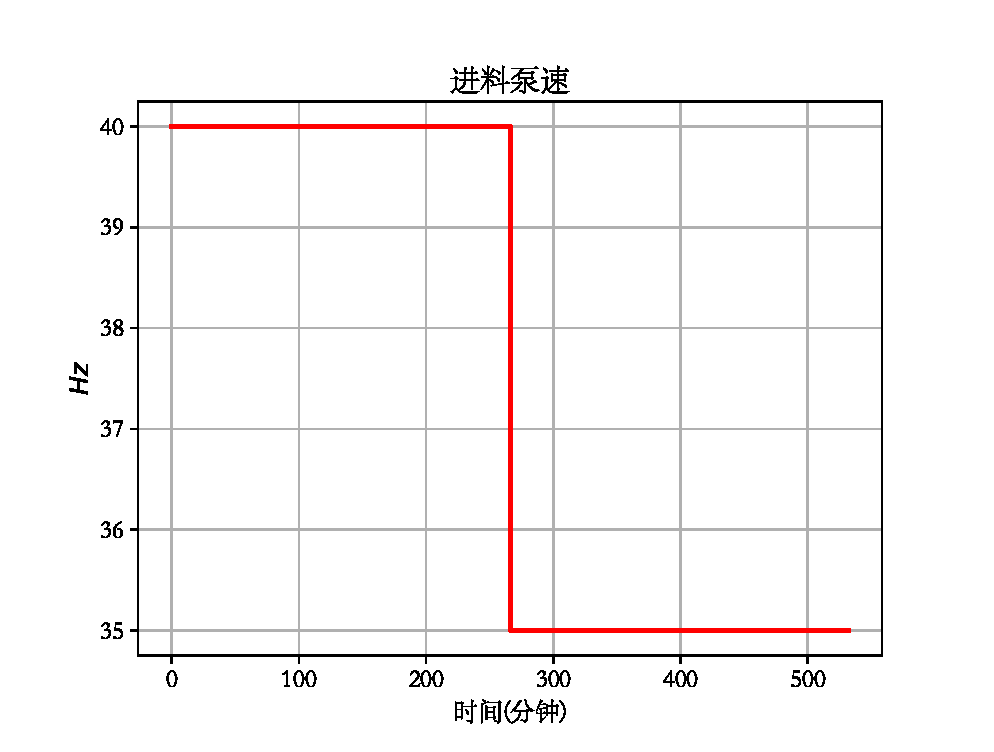
\includegraphics[width=0.49\linewidth,trim=18 0 23 0,clip]{figures/chapter6/fig6a.eps}}
% \subfigure{\label{fig:subfigure2}} \addtocounter{subfigure}{-2}
% \subfigure[Concentration of feed changes suddenly.]
{\subfigure[进料浓度变化.]
{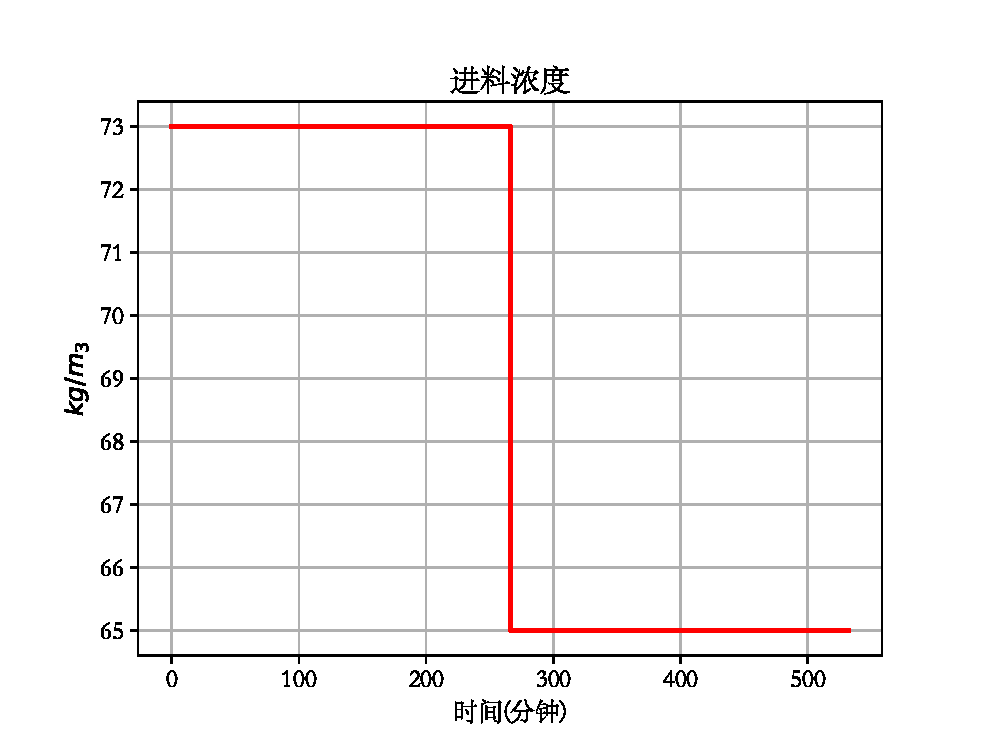
\includegraphics[width=0.49\linewidth,trim=18 0 23 0,clip]{figures/chapter6/fig6b.eps}}}
\caption{噪音量变化曲线}
% %%%%%%%%%%%%%英文标题begin
%   \addtocounter{figure}{-1}
%   \vspace{-5pt}
%   %\SetEnglishCaption
%   % \renewcommand{\figurename}{Fig.}
%   % \caption{Noise input in the simulation experiment}
%   \renewcommand{\figurename}{图}
%%%%%%%%%%%%%英文标题end
\label{fig:stable_noise_input}
\end{figure}


%\begin{figure}[ht]
%\centering
%\subfigure[进料泵速变化. Speed of feed pump changes
%suddenly.]{
%  \includegraphics[width=3.9cm]{vi_hdp_stable/JLBS_HDP_HCNVI.eps}
%  \label{fig:subfigure1}}
%  \subfigure[进料浓度变化. Concentration of feed changes suddenly.]{
% \includegraphics[width=3.9cm]{vi_hdp_stable/JLND_HDP_HCNVI.eps}
%  \label{fig:subfigure2}
%  }
%%
%\caption{噪音量变化曲线}
%%%%%%%%%%%%%%英文标题begin
%  \addtocounter{figure}{-1}
%  \vspace{-5pt}
%  %\SetEnglishCaption
%  \renewcommand{\figurename}{Fig.}
%  \caption{Noise input in the simulation experiment}
%  \renewcommand{\figurename}{图}
%%%%%%%%%%%%%%英文标题end
%\label{fig:stable_noise_input}
%\end{figure}

使用本章提出的HCNVI算法与HDP、DHP、ILPL算法进行对比实验。
仿真实验参数如下:迭代轮次$T=270$, 仿真步长$T_d\sim \mathbb{U}(60s, 180s)$, $Q=0.004$,
%$R=diag\{0.001,0.008\}$,
$\gamma=0.6$, $N_a=4000$, $N_c=500$, $\epsilon _c=0.001$,
$\epsilon _a=0.0001$, $l_m=0.01$, $l_c=0.01$, $l_a=0.009$,
$l_u=0.4$, $L_c=2$, $\b {L_m}=[0.01,3]$。
其中HDP、DHP算法也使用短期经验回放,回放点数$L$为2。实验中HDP、ILPL、HCNVI的评价网络结构相同,且网络参数初始化为相同数值。实验结果如图\ref{fig:HCNVI_HDP}所示。
\begin{figure}[htb]
\centering \subfigure{\label{fig:concentraion_out_exp1}}
% \addtocounter{subfigure}{-2} \subfigure[Concentration of underflow.]
{\subfigure[底流浓度变化.]
{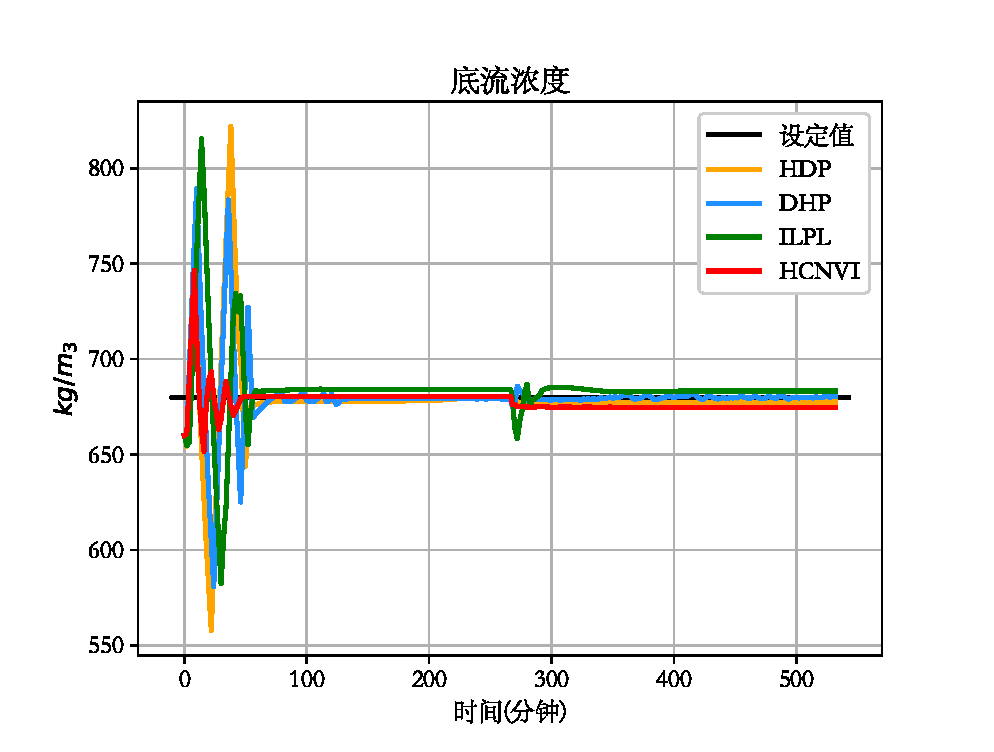
\includegraphics[width=0.49\linewidth,trim=18 0 23 0,clip]{figures/chapter6/fig7a.eps}}} \centering
 \subfigure{\label{fig:cost_exp1}}
% \addtocounter{subfigure}{-2} \subfigure[Utility.]
{\subfigure[效用函数值变化.]
{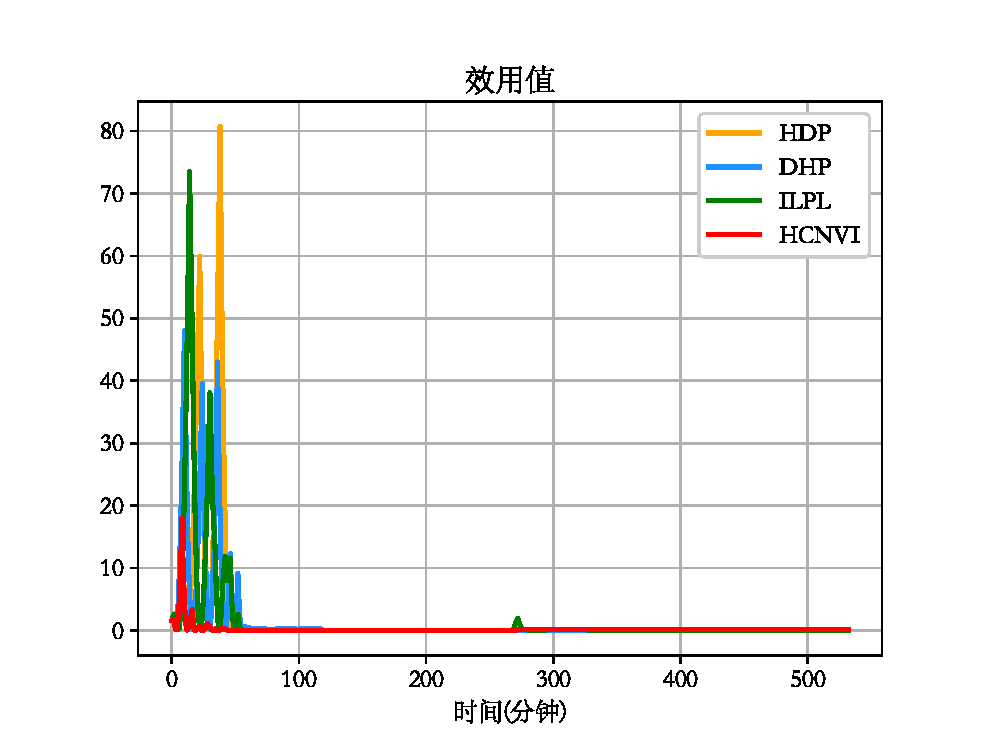
\includegraphics[width=0.49\linewidth,trim=18 0 23 0,clip]{figures/chapter6/fig7b.eps}}}
    \caption{HCNVI与其他ADP算法在恒定噪音输入下的对比}
%%%%%%%%%%%%%英文标题begin
  \addtocounter{figure}{-1}
  \vspace{-5pt}
  %\SetEnglishCaption
  % \renewcommand{\figurename}{Fig.}
  % \caption{HCNVI versu other ADP algorithms under stable noisy input}
  \renewcommand{\figurename}{图}
%%%%%%%%%%%%%英文标题end
    \label{fig:HCNVI_HDP}
\end{figure}

% \begin{figure}
%   \centering
%   \hspace{-0.1in}
%   \subfigure[State-\textit{off}]{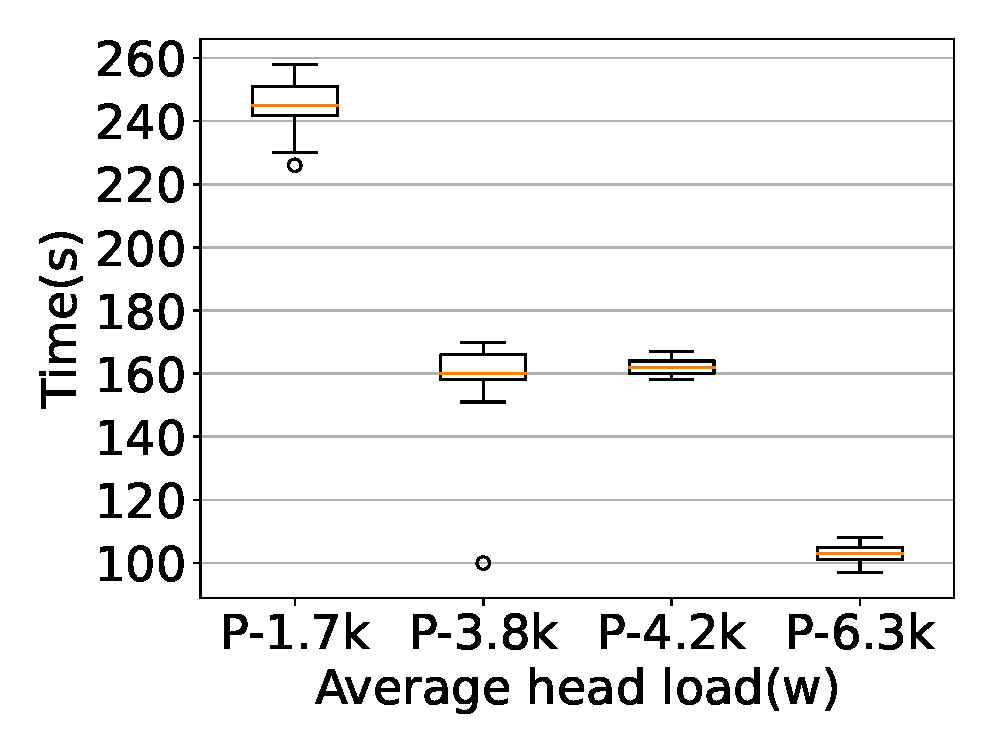
\includegraphics[width=0.45\linewidth,\linewidth,trim=18 0 23 0]{figures/chapter4/state1.eps}}\hspace{-0.05in}
%   \subfigure[State-\textit{on}]{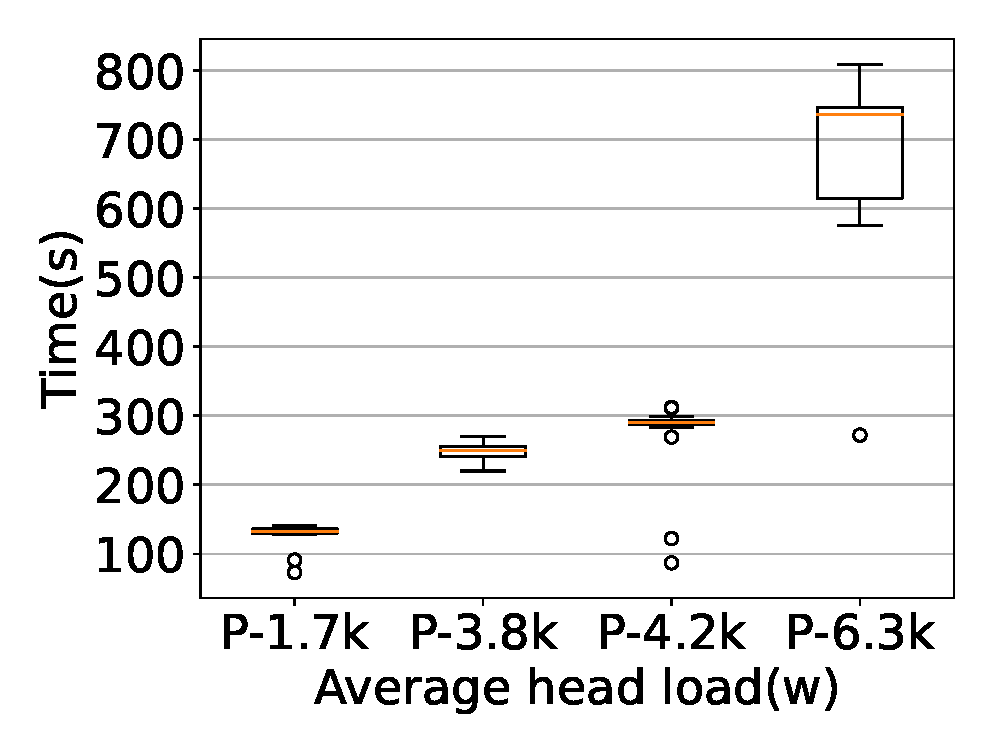
\includegraphics[width=0.45\linewidth,\linewidth,trim=18 0 23 0]{figures/chapter4/state4.eps}}
%   \caption{
%   % The data of the four data sets are generated at different power of the server, which are 1.7kw, 3.8kw, 4.2kw and 6.3kw respectively. Compare the duration time of system on and off   under different power.
%   在平均负载不同的四个数据集中,阶段\textit{On}和\textit{Off}的持续时间分布箱线图
%   } %图片标题
%   \label{fig:HCNVI_HDP}  %图片交叉引用时的标签
%   \end{figure}


根据实验结果可以发现,对于不同控制算法,由于网络参数初始值均为随机设定值,训练初期底流浓度有较大幅度的波动,且在设定值两侧持续震荡。
随着各个控制模型的学习,系统状态与网络参数不断趋于平稳,直到某一时刻底流浓度开始稳定并与设定值重合且不再产生波动,此时控制模型参数也不再发生变化,被控系统和控制模型同时收敛到最优态。
从效用值变化曲线也可以看出,早期由于底流浓度与其设定值偏差较大,效用值较高。但是随着模型与系统趋于稳态,效用值${U}(t)$不断减小直到接近于0的位置。
%
到达270分钟时,系统进料浓度、进料流量发生突变,底流浓度无法维持稳态,开始远离设定值。控制模型根据噪音量改变后的系统所产生的轨迹数据重新训练,将底流浓度拉回设定值位置。由于在第一阶段控制模型已经到达过一次稳态,在第二阶段仅需要少量迭代就可以使系统重归理想收敛稳态。
通过观察不同控制算法产生的系统轨迹,可以发现不同控制算法到达最优态所需的时间有较大差别,且在收敛到最优态的过程中,底流浓度的波动也有较大差异。
在实验第一阶段,为使系统达到稳态,HCNVI算法所需要的迭代次数更少,训练过程中产生的底流浓度振幅也更小。并且在噪音量改变后,HCNVI算法可以迅速地使模型重归最优态,且底流浓度几乎未发生大幅度波动。

HCNVI的快速收敛能力主要来源于其采用迭代算法\ref{alg:find_optimal_policy}得出的${\b
u}(k)$严格满足\equref{equ:VI_u}的最小化条件,可以使评价网络更快地收敛到最优评价值函数。而其他ADP算法中引入了动作网络,这会使策略的更新存在一定的滞后性,进而拖慢评价网络的训练速度。
% HCNVI算法直接根据当前的评价网络求解最优的控制动作,可以使评价网络更快地收敛到最优评价值函数。
%由于浓密机系统常处于噪音频繁波动环境,控制模型需要快速适应被控系统的变化,因此HCNVI相比于ADP算法更适合用于工业过程控制场景。

为了验证短期经验回放技术对控制算法性能的影响,本章分别对比了无经验回放、使用短期经验回放($L=2$)情况下HDP、HCNVI的控制性能。
对比结果如图\ref{fig:stable_replay_cmp}所示。
在本实验中,仅比较了两种算法的效用值变化,效用值越快地收敛到0说明算法控制效果越佳。通过观察图\ref{fig:stable_replay_cmp}中无经验回放情况下的效用值变化曲线,可以发现曲线波动较大。相比于使用短期经验回放,无经验回放情况下控制模型需要更多的迭代轮次才能够使系统达到收敛。
特别是在图\ref{fig:noise_HCNVI_HDP}\subref{fig:concentraion_out_exp1}的HCNVI的实验中,270分钟时系统噪音输入量改变,效用值开始剧增,底流浓度开始偏离设定值,评价网络的学习结果如图\ref{fig:replay_compare}\subref{fig:6_no_replay}中的第四部分所示。评价网络对当前状态点$\b
x(k)$的局部梯度估计有较大偏差,使得利用算法\ref{alg:find_optimal_policy}求解的${\b u}(k)$并没有驱使底流浓度向其设定值移动,被控系统无法收敛。但在增加了短期经验数据回放后,无论是本章提出的HCNVI算法还是HDP算法,效用函数值可以快速收敛至最低点,有效实现对被控系统的控制。
该实验结果表明短期经验回放技术对于控制模型的收敛速度改善效果明显,且对不同ADP算法具有通用型。


\begin{figure}[htb]
\centering 
% \subfigure{\label{fig:hdp_exp1_replay_stable}}
% \addtocounter{subfigure}{-2} \subfigure[Short-term experience replay
% has great influence to minimize the utility in HDP.]
\subfigure[在HDP算法中引入经验回放对效用值的影响.]
{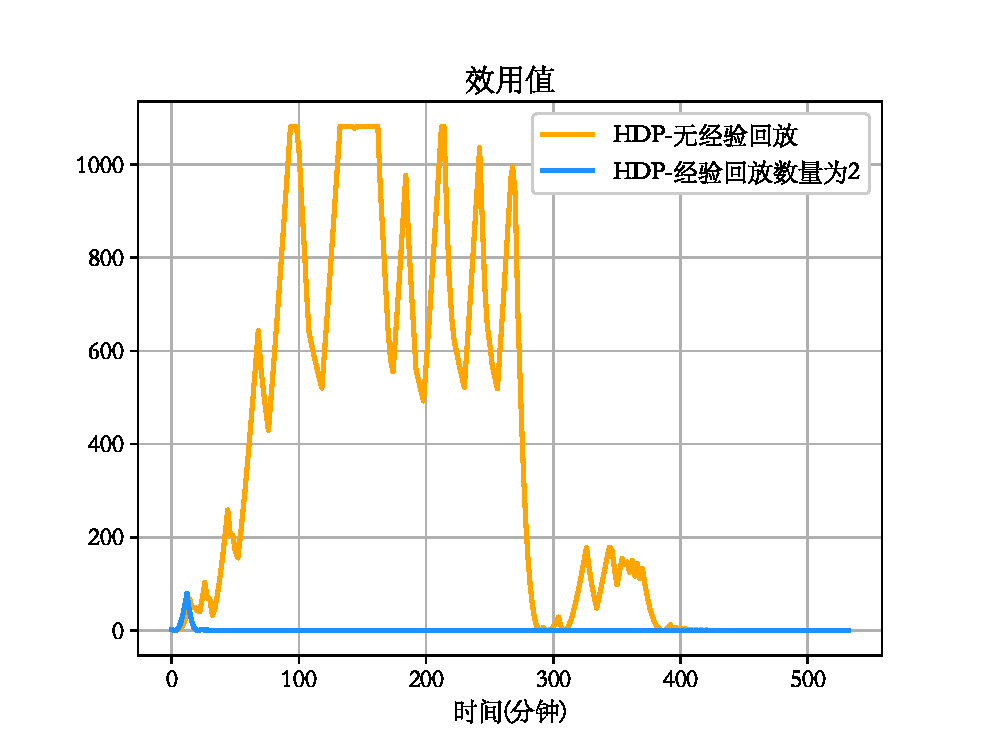
\includegraphics[width=0.49\linewidth,trim=18 0 23 0,clip]{figures/chapter6/fig8a.eps}} 
%  \subfigure{\label{fig:hcnvi_exp1_replay_stable}}
% \addtocounter{subfigure}{-2} \subfigure[Short-term experience replay
% has great influence to minimize the utility in HCNVI.]
\subfigure[在HCNVI算法中引入经验回放对效用值的影响.]
{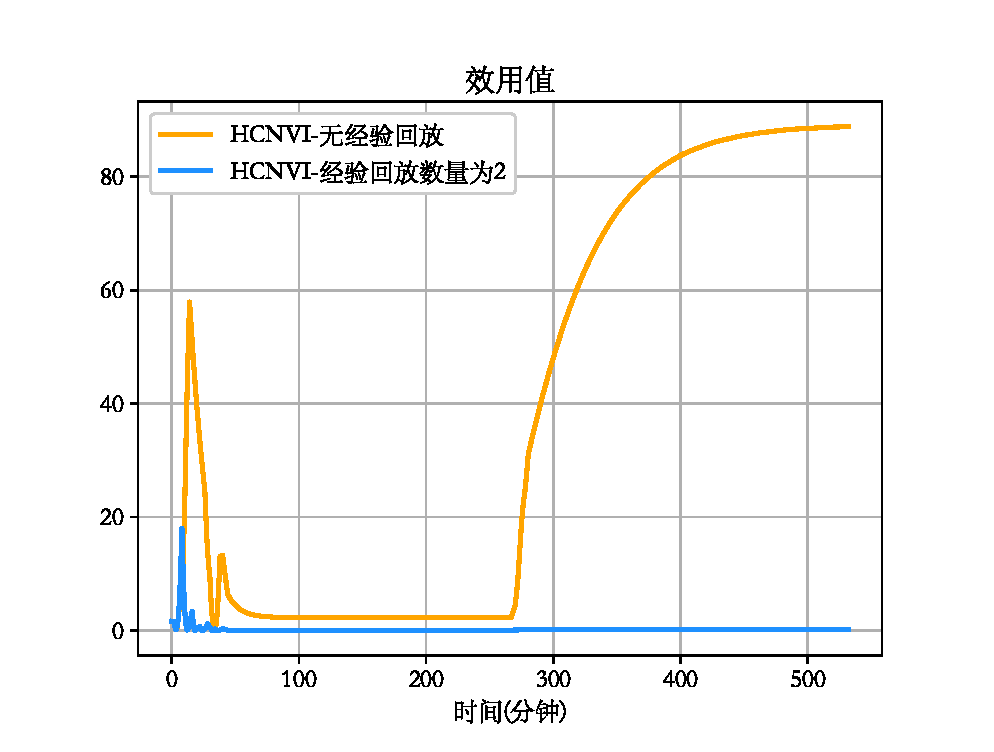
\includegraphics[width=0.49\linewidth,trim=18 0 23 0,clip]{figures/chapter6/fig8b.eps}}
    \caption{短期经验回放对HDP与HCNVI的影响 }
%%%%%%%%%%%%%英文标题begin
  % \addtocounter{figure}{-1}
  % \vspace{-5pt}
  % %\SetEnglishCaption
  % \renewcommand{\figurename}{Fig.}
  % \caption{The influence of short-term experience replay on HDP and HCNVI}
  % \renewcommand{\figurename}{图}
%%%%%%%%%%%%%英文标题end
    \label{fig:stable_replay_cmp}
\end{figure}

另外本章进行了十组实验来对比HCNVI算法在时间上的优势。选取HDP算法作为参考对象。
% 用于耗时比较的处理器型号为2.6GHz、六核Intel Core i7。
实验用机的CPU型号为2.6GHz、六核Intel Core i7,网络均采用CPU进行训练。
仿真时间为$T=270$,结果如图\ref{fig:time_cmp}\subref{fig:stable_time_cmp}所示。
由于每次实验中网络初始值不同,系统运行轨迹以及模型训练过程也不同,因此每组实验中模型学习以及控制所需的累积时间略有差异。
% 但是从多次实验结果可以看出,HDP算法利用动作网络正向计算求解控制输入量几乎是不耗时的。
% HCNVI算法在求解控制动作时由于需要不断迭代,消耗的时间多于HDP算法。
% 但由于在HCNVI算法中,仅评价网络需要训练,使得其在模型训练环节上所花费的时间大大削减,总时间消耗上明显优于HDP算法。
但是从多次实验结果可以看出,由于
HCNVI算法中去掉了动作网络,仅需要训练评价网络,所以模型整体训练时间大大缩减,尽管算法\ref{alg:find_optimal_policy}中计算控制输入所需时间相比于HDP算法直接利用动作网络前向传播求解控制动作所需时间长,但是HCNVI算法总消耗时间明显少于HDP算法。

前人研究表明,在启发式动态规划类算法中,去掉动作网络可以有效减少模型训练时间\cite{Luo2016,Padhi2006}。
但是在某些复杂系统控制问题中,去除动作网络会使模型难以拟合复杂策略函数,最终导致控制效果变差。在本章的实验环节中,由于浓密机系统运行缓慢且具有较高时滞性,当前时刻控制输入量${\b
u}(k)$对$\hat{\b x}(k+1)$的影响较小,即对$\hat{J}(k)$的影响较小。
因此利用算法\ref{alg:find_optimal_policy}求解的${\b
u}(k)$满足\equref{equ:VI_u}的最小化条件。
而在HDP、DHP、ILPL等方法中采用神经网络拟合出的控制策略,难以输出严格满足\equref{equ:VI_u}的${\b
u}(k)$,算法\ref{alg:find_optimal_policy}的最优性代表HCNVI可以最大程度地利用评价网络给出的协状态信息优化当前控制策略,进而获得更高的控制效果。但HCNVI方法也具有一定的局限性,当被控系统状态变化速率较快,$\hat{J}(k)$随${\b
u}(k)$变化的分布函数不再是单峰函数,算法\ref{alg:find_optimal_policy}求解出的${\b
u}(k)$极容易陷入到局部最优解,算法控制效果及收敛速度必然变差。
而此时在HDP、DHP、ILPL等方法中采用神经网络拟合的控制策略往往能够给出相对更优、鲁棒性更强的控制动作${\b
u}(k)$,其控制效果与收敛速率必然优于HCNVI算法。



% 在某些实时性要求较高的工业控制场景中,削减时间损耗是极其重要的。

% \begin{figure}[htb]
%     \centering
%     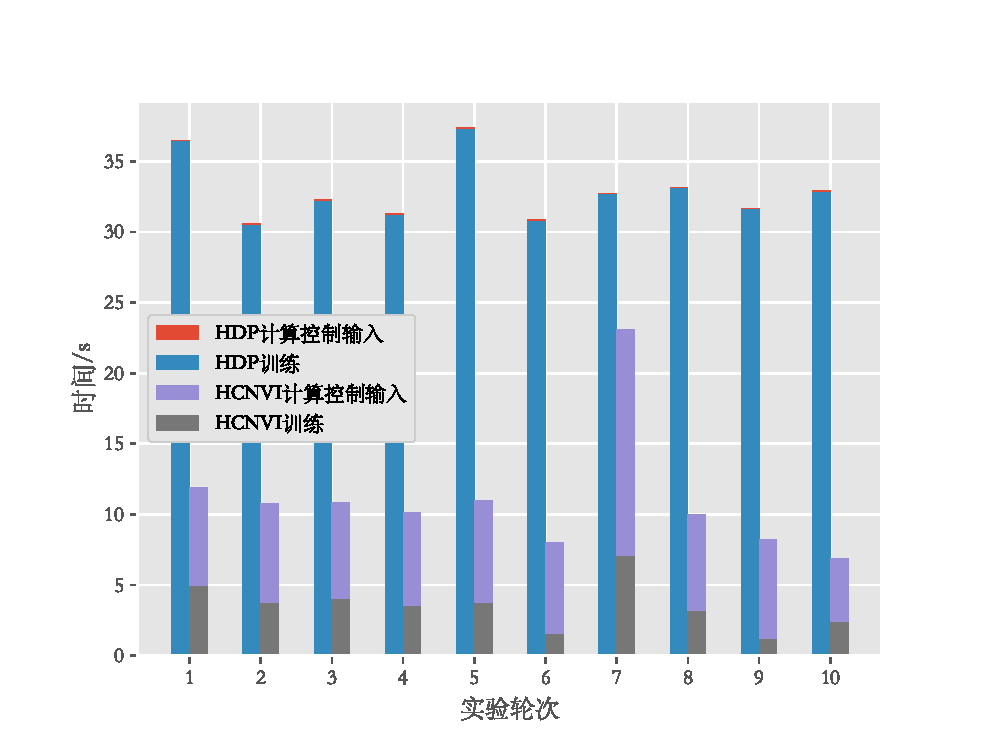
\includegraphics[width=0.7\linewidth]{figures/chapter6/fig9.eps}
%     \caption{实验一中HDP与HCNVI在时间消耗上的对比 }
% % %%%%%%%%%%%%%英文标题begin
% %   \addtocounter{figure}{-1}
% %   \vspace{-5pt}
% %   %\SetEnglishCaption
% %   \renewcommand{\figurename}{Fig.}
% %   \caption{Comparison of time consuming in HDP and HCNVI in experiment 1}
% %   \renewcommand{\figurename}{图}
% % %%%%%%%%%%%%%英文标题end
%     \label{fig:stable_time_cmp}
% \end{figure}
\begin{figure}[htb]
  % \centering
  %  \subfigure{\label{fig:noise_noise_input1}}
  % \addtocounter{subfigure}{-2} \subfigure[The speed of feed pump
  % varies in real time.] {
    \subfigure[恒定噪音输入]
  {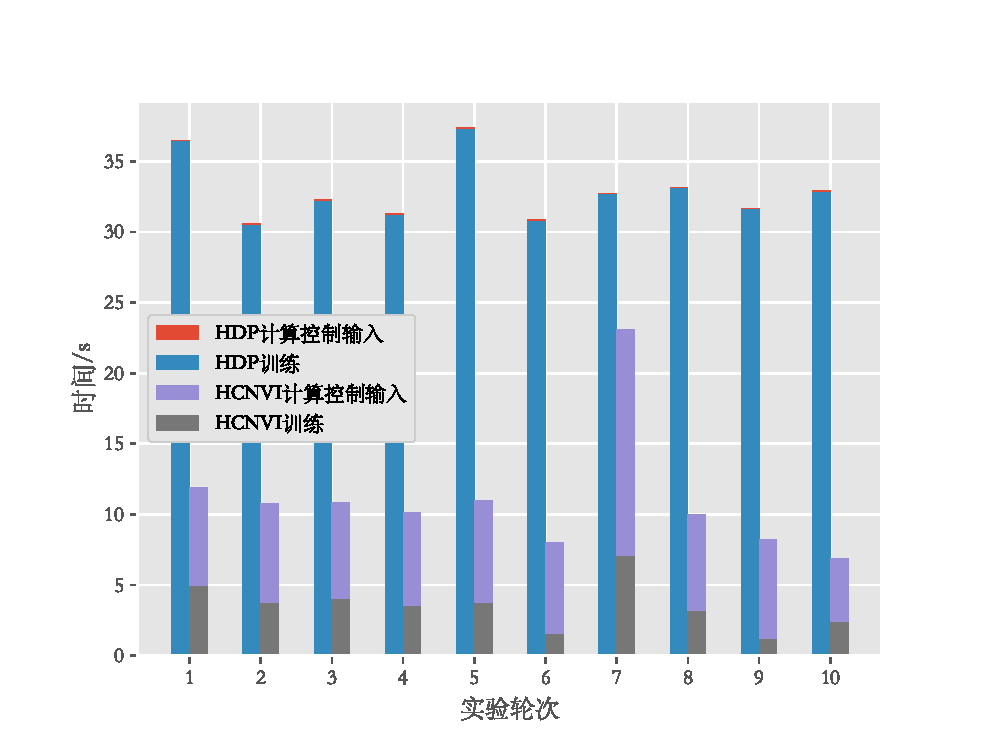
\includegraphics[width=0.49\linewidth,trim=18 0 23 0,clip]{figures/chapter6/fig9.eps} 
  \label{fig:stable_time_cmp}
  }
  %  \subfigure{\label{fig:noise_noise_input2}}
  % \addtocounter{subfigure}{-2} \subfigure[The feed concentration
  % varies in real time.] 
  \subfigure[随机噪音输入]
  {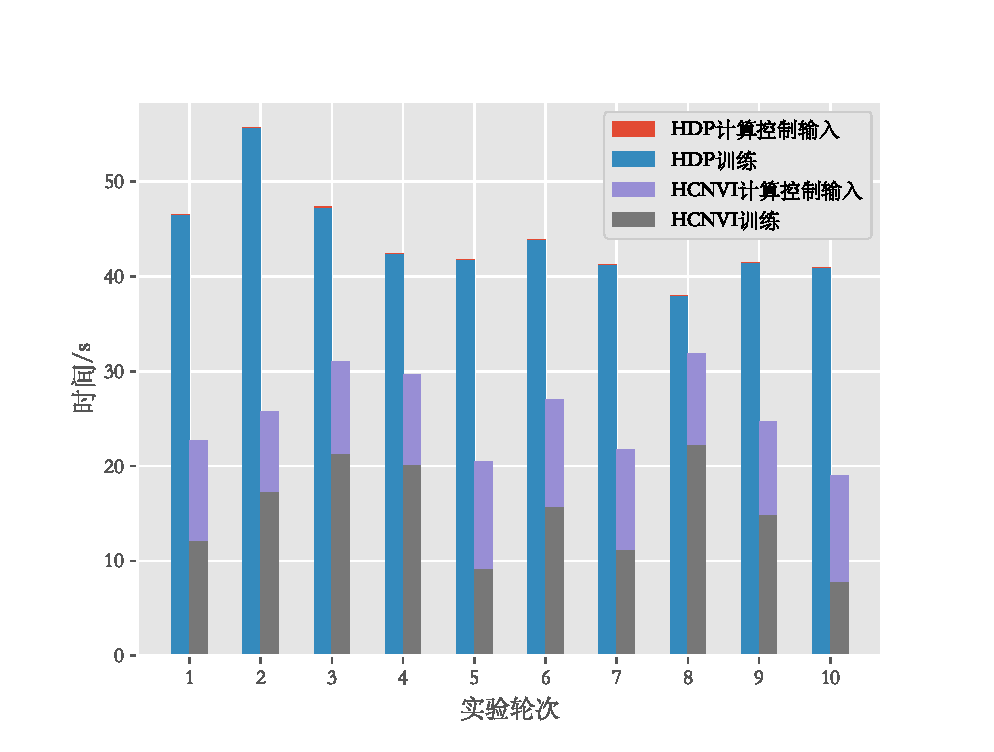
\includegraphics[width=0.49\linewidth,trim=18 0 23 0,clip]{figures/chapter6/fig13.eps} 
  \label{fig:noise_time_cmp}
  }
      \caption{HDP与HCNVI在时间消耗上的对比}
  %%%%%%%%%%%%%英文标题begin
    % \addtocounter{figure}{-1}
    % \vspace{-5pt}
    % %\SetEnglishCaption
    % \renewcommand{\figurename}{Fig.}
    % \caption{The fluctuation of noisy input}
    % \renewcommand{\figurename}{图}
  %%%%%%%%%%%%%英文标题end
      \label{fig:time_cmp}
  \end{figure}



\subsection{高斯噪音波动输入下浓密机控制仿真实验}
\label{sec:vi_hdp_noise}
实验一中仿真模型的进料状态是恒定的,只在某一时刻产生突变,其目的是为了更好地观察不同控制算法的收敛速度。而真实工业场景下,浓密机的进料浓度和进料流量是实时波动的。
在本节实验中,进料流量和进料浓度两个噪音量持续波动,用来模仿真实工业场景下的浓密机系统环境。
噪音输入的单步变化增量服从高斯分布,进料波动变化如图\ref{fig:noise_noise_input}所示。
\begin{equation}
%\begin{align*}
\begin{split}
%\centering
 \label{equ:noise_c_disturbance}
 \b c(k+1) =&\b c(k)+\Delta \b c \\
 \Delta \b c \sim N(\mu=0 ,
\Sigma&=\operatorname{diag}(0.6,0.6))
%\centering
\end{split}
%\end{align*}
\end{equation}

本实验中HCNVI控制器参数与实验一\ref{sec:vi_hdp_stable}节中的算法参数相同,迭代轮次$T=270$,
仿真步长$T_d=120s$。
\begin{figure}[htb]
% \centering
%  \subfigure{\label{fig:noise_noise_input1}}
% \addtocounter{subfigure}{-2} \subfigure[The speed of feed pump
% varies in real time.] {
  \subfigure[进料泵速变化.]
{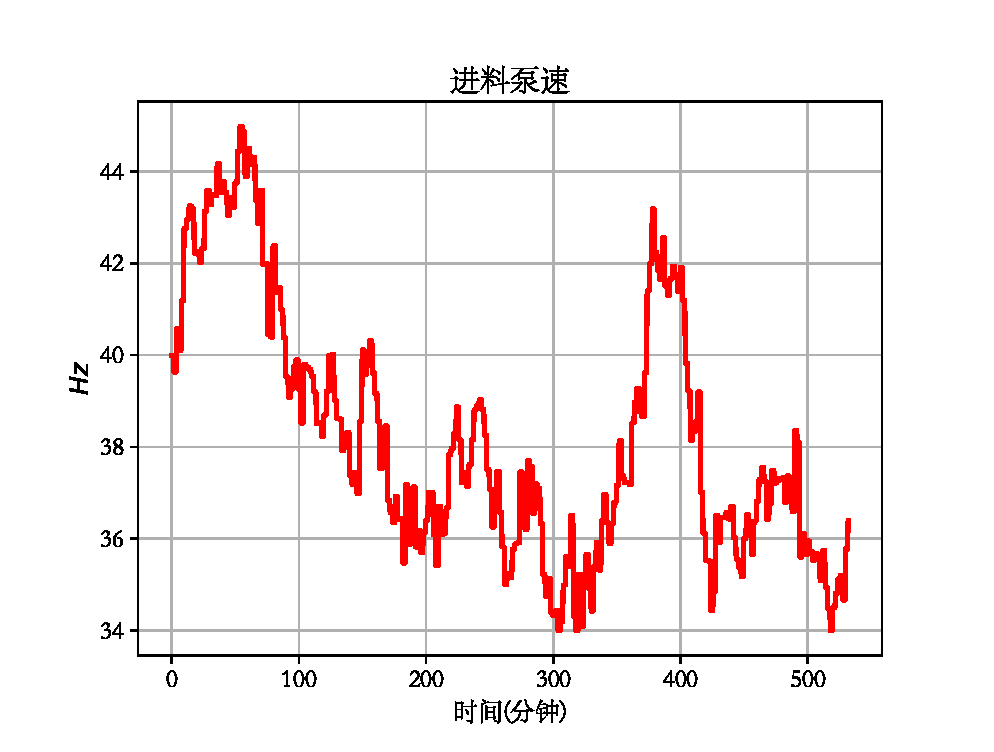
\includegraphics[width=0.49\linewidth,trim=18 0 23 0,clip]{figures/chapter6/fig10a.eps} }
%  \subfigure{\label{fig:noise_noise_input2}}
% \addtocounter{subfigure}{-2} \subfigure[The feed concentration
% varies in real time.] 
\subfigure[进料浓度变化. ]
{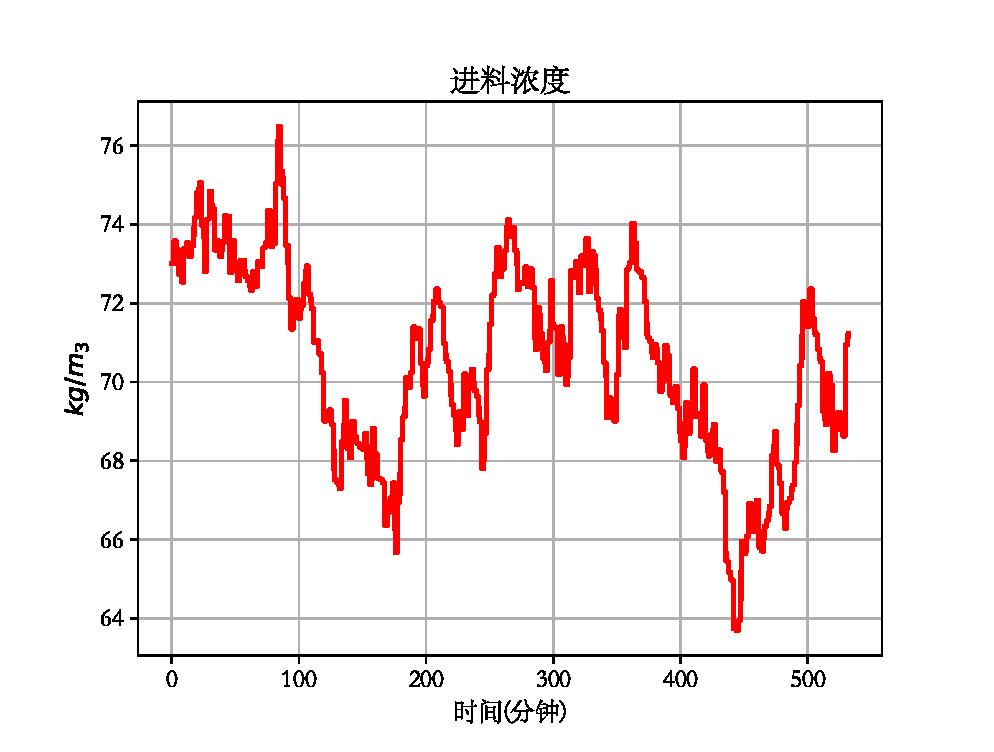
\includegraphics[width=0.49\linewidth,trim=18 0 23 0,clip]{figures/chapter6/fig10b.eps} }
    \caption{噪音量变化曲线}
%%%%%%%%%%%%%英文标题begin
  % \addtocounter{figure}{-1}
  % \vspace{-5pt}
  % %\SetEnglishCaption
  % \renewcommand{\figurename}{Fig.}
  % \caption{The fluctuation of noisy input}
  % \renewcommand{\figurename}{图}
%%%%%%%%%%%%%英文标题end
    \label{fig:noise_noise_input}
\end{figure}
利用该仿真模型再次对比HCNVI与其他算法控制性能的差异,结果如图\ref{fig:noise_HCNVI_HDP}所示。
\begin{figure}[htb]
\centering 
% \subfigure{}
% \addtocounter{subfigure}{-2} \subfigure[ Concentration of
% underflow.] 
\subfigure[底流浓度变化.]
{\label{fig:concentraion_out_exp1_noise}
  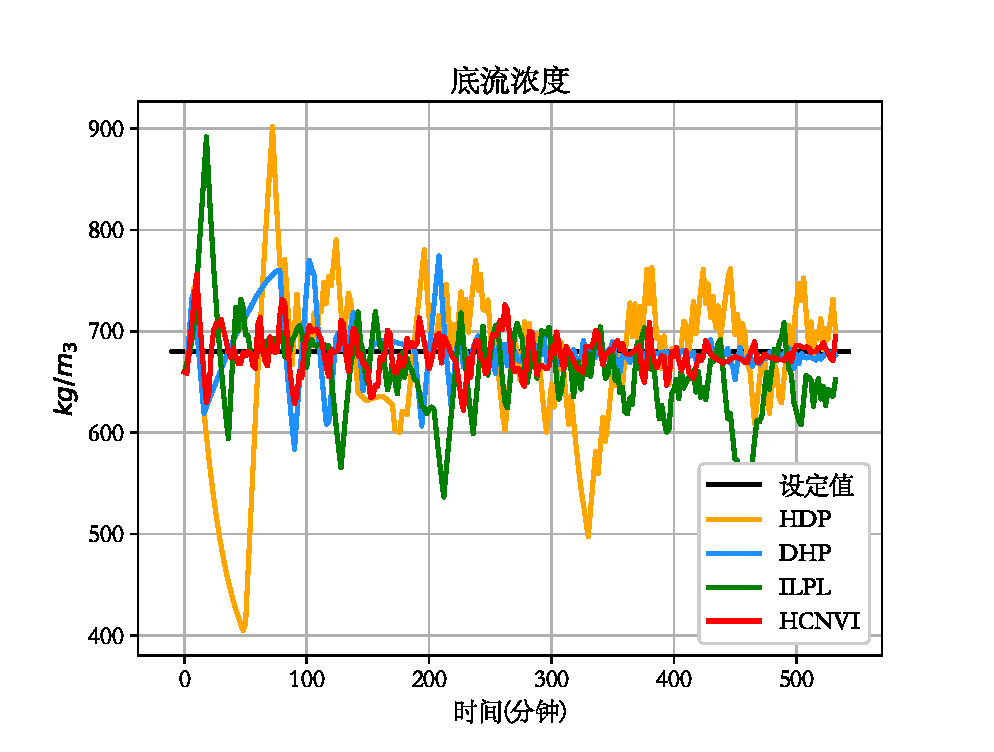
\includegraphics[width=0.49\linewidth,trim=18 0 23 0,clip]{figures/chapter6/fig11a.eps}}
\subfigure[效用函数值变化.]
{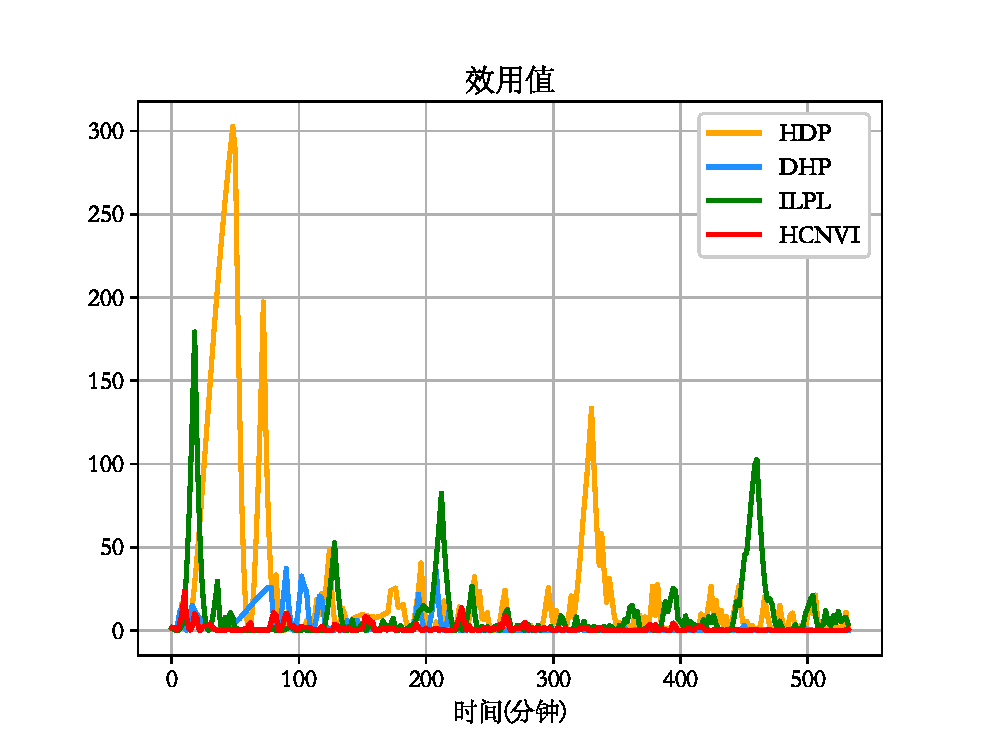
\includegraphics[width=0.49\linewidth,trim=18 0 23 0,clip]{figures/chapter6/fig11b.eps}}
\caption{HCNVI与其他ADP算法在波动噪声输入下的对比}
%%%%%%%%%%%%%英文标题begin
  % \addtocounter{figure}{-1}
  % \vspace{-5pt}
  % %\SetEnglishCaption
  % % \renewcommand{\figurename}{Fig.}
  % % \caption{HCNVI versu other ADP algorithms under fluctuate noisy input}
  % \renewcommand{\figurename}{图}
%%%%%%%%%%%%%英文标题end
    \label{fig:noise_HCNVI_HDP}
\end{figure}


通过观察实验结果发现在环境噪音连续变化条件下,浓密机底流浓度会发生持续震荡。随着对模型参数的不断训练,各个算法的控制性能趋于平稳,由于进料噪音导致的底流浓度波动稍有减弱。
对比不同控制算法的控制性能,可以发现HCNVI相比于其他ADP算法能够更快地将底流浓度锁定在设定值邻域范围内,且浓度振幅小于其他算法。
从效用值变化曲线也可以看出,相比于其他算法,HCNVI算法的效用值整体较小,且在训练后期几乎0。

该实验结果与实验一\ref{sec:vi_hdp_stable}中进料噪音突变条件下的实验结果相吻合。
HCNVI算法在外界噪音频繁改变时,可以更快地响应外部变化,快速调节评价网络参数,将底流浓度稳定在目标值附近。其他算法由于增加了动作网络产生了训练滞后性,进而导致无法快速适应外部环境的变化,使其控制性能差于HCNVI。

\tabref{tab:MSE_cmp}给出了不同算法在实验一\ref{sec:vi_hdp_stable}和实验二\ref{sec:vi_hdp_noise}节中底流浓度控制性能指标对比结果。
相比其他算法,HCNVI算法可以更好地控制底流浓度稳定在其设定值附近,其控制总体稳定性(由MSE、IAE体现)、控制鲁棒性(由MAE体现)更佳。在过程工业控制场景中,控制系统的MAE指标尤为重要,某一工序的物料性质发生剧烈波动会使下游物料加工工序出现连带波动,严重影响生产的稳定性和最终产品的质量。HCNVI算法在MAE指标上的优势证实了其在过程工业控制问题中的适用性。


% Please add the following required packages to your document preamble:
% \usepackage{graphicx}
\begin{table*}[htb]

\caption{不同控制算法之间性能分析}
 %英文标题begin
    % \addtocounter{table}{-1}
    % \vspace{-0.2cm}
    %\SetEnglishCaption
    % \renewcommand{\tablename}{Table}
    % \caption{Performances analysis of different algorithms}
    % \renewcommand{\tablename}{表}
    % \vspace{0.4cm}
 %英文标题end
%\resizebox{\textwidth}{!}{%
\begin{tabular}{l|lll|lll}
\toprule
实验组 & \multicolumn{3}{c|}{实验一(恒定噪音)} & \multicolumn{3}{c}{实验二(随机噪音)} \\
\hline 对比指标 & \multicolumn{1}{c}{MSE\footnotemark[1]} &
\multicolumn{1}{c}{MAE\footnotemark[2]} &
\multicolumn{1}{c|}{IAE\footnotemark[3]} & \multicolumn{1}{c}{MSE} &
\multicolumn{1}{c}{MAE} & \multicolumn{1}{c}{IAE} \\ \hline
HDP & 414.182& 141.854 & 7.246 & 6105.619 & 275.075 & 54.952 \\
DHP & 290.886 & 109.312 & 5.392 & 732.814 & 96.145 & 16.560 \\
ILPL & 364.397 & 135.474 & 8.289 & 2473.661 &211.615 & 35.222 \\
\textbf{HCNVI} & \textbf{44.445} & \textbf{66.604} & \textbf{3.867} & \textbf{307.618} & \textbf{76.176} & \textbf{12.998} \\
\bottomrule
\end{tabular}%
%}
\label{tab:MSE_cmp} \centering
\end{table*}

\footnotetext[1]{平均平方误差(Mean Square Error, MSE)=$\frac{1}{T} \sum_{k=1}^{T}\left|(y(k)-y^*(k))\right|^{2}$} \footnotetext[2]{最大绝对误差(Max Absolute Error,MAE)=$\max _{1 \leq k \leq T}\{|y(k)-y^*(k)|\}$} \footnotetext[3]{累积绝对误差(Integral Absolute Error, IAE)=$\frac{1}{T} \sum_{k=1}^{T}\left|(y(k)-y^*(k))\right|$}


图\ref{fig:noise_replay_cmp}展示在环境噪音持续变化条件下,不使用经验回放和使用短期经验回放($L=2$)两种情况下HCNVI算法控制性能。
在无经验回放情况下,底流浓度稳定性明显较差,且效用值明显较高,使用短期经验回放($L=2$)后模型控制效果较好。
实验结果表明,短期经验回放技术在环境噪音持续变化下仍对模型控制效果与收敛速度有重要促进作用。

\begin{figure}[htb]
% \centering \subfigure{\label{fig:cost_exp1_replay_noise}}
% \addtocounter{subfigure}{-2} \subfigure[The influence of short-term
% experience replay on underflow concentration for HCNVI.]
\subfigure[在HCNVI算法中引入经验回放对底流浓度的影响.]
{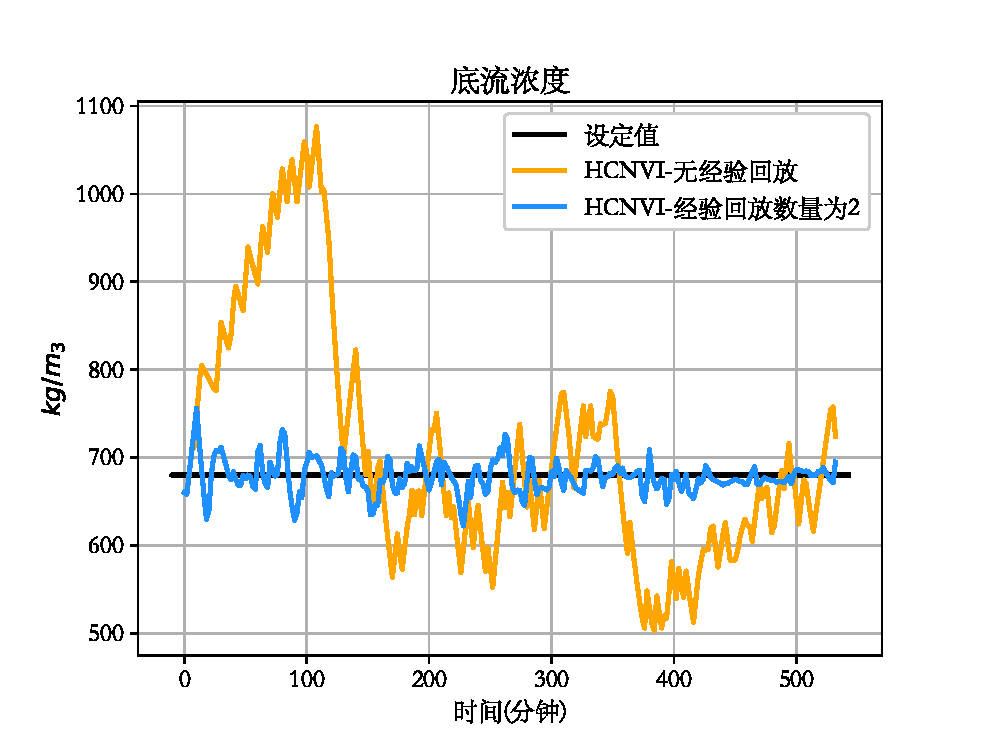
\includegraphics[width=0.49\linewidth,trim=18 0 23 0,clip]{figures/chapter6/fig12a.eps} }
% \subfigure{\label{fig:concentraion_out_exp1_replay_noise}}
% \addtocounter{subfigure}{-2} \subfigure[The influence of short-term
% experience replay on utility for HCNVI.]
\subfigure[在HCNVI算法中引入经验回放对效用值的影响.]
{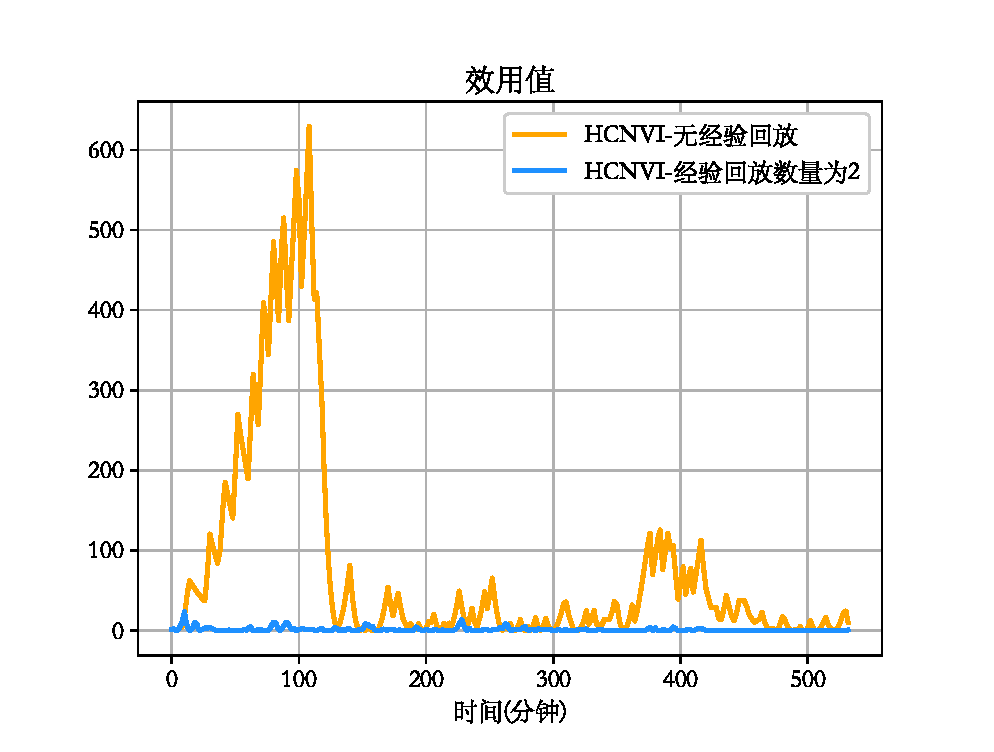
\includegraphics[width=0.49\linewidth,trim=18 0 23 0,clip]{figures/chapter6/fig12b.eps} } 
\caption{噪音持续变化下短期经验回放对HCNVI的影响 }
%%%%%%%%%%%%%英文标题begin
  % \addtocounter{figure}{-1}
  % \vspace{-5pt}
  % %\SetEnglishCaption
  % % \renewcommand{\figurename}{Fig.}
  % % \caption{The influence of short-term experience replay on HCNVI}
  % \renewcommand{\figurename}{图}
%%%%%%%%%%%%%英文标题end
    \label{fig:noise_replay_cmp}
\end{figure}

为了展现在噪音持续变化条件下,HCNVI算法在时间上的优势,再次重复了十次实验对比了HCNVI算法与HDP算法的时间消耗,$T=270$。
实验结果如图\ref{fig:time_cmp}\subref{fig:noise_time_cmp}所示。在噪音持续变化环境下,HCNVI
算法和HDP算法的总时间消耗相比于图\subref{fig:stable_time_cmp}中的结果均有增加。这是由于当外部环境存在持续扰动时,被控系统和控制模型参数不再如实验一\ref{sec:vi_hdp_stable}节中达到稳定态,而是始终处于震荡状态,被控系统轨迹数据不断变化。每轮学习过程中,为了满足评价网络的精度$e_{c}(k)^{2}<\epsilon_{c}$
所需要的训练迭代次数增加,进而导致评价网络训练所需时间及模型总体训练时间增加。
但通过横向对比HCNVI算法与HDP算法的总时间消耗,HCNVI算法在训练和执行控制过程中所需的总时间消耗仍明显少于HDP,说明利用算法\ref{alg:find_optimal_policy}替代动作网络所减少的时间消耗在噪音连续波动条件仍十分明显。


% \begin{figure}[htb]
%     \centering
%     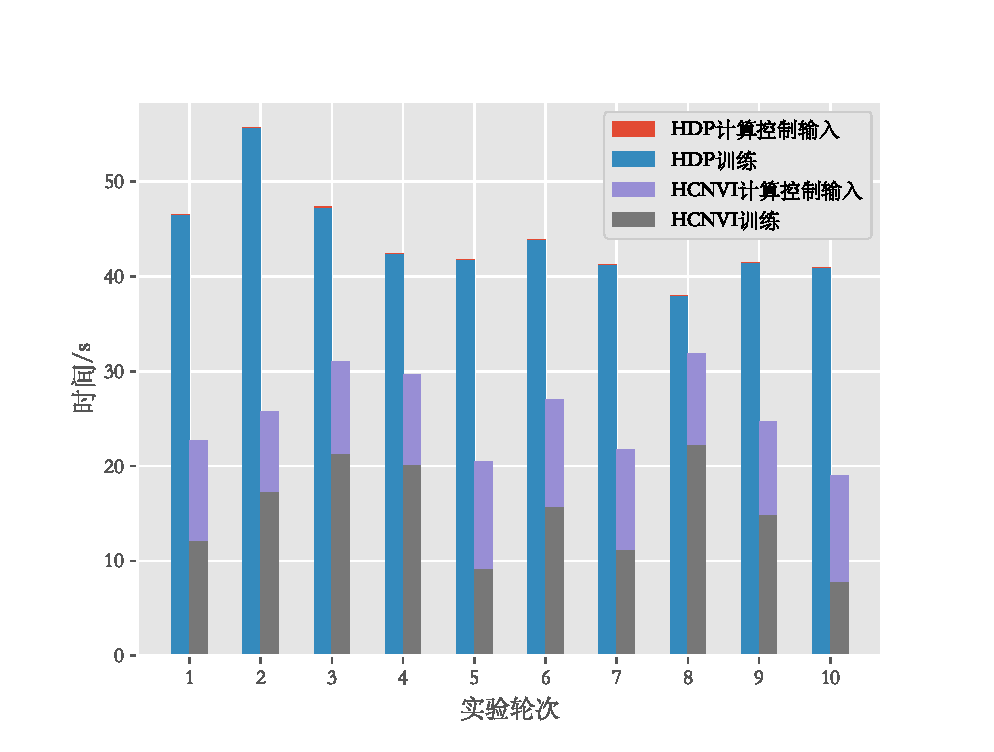
\includegraphics[width=0.9\linewidth]{figures/chapter6/fig13.eps}
%     \caption{实验二中HCNVI算法与HDP算法在时间消耗上的对比}
% %%%%%%%%%%%%%英文标题begin
%   \addtocounter{figure}{-1}
%   \vspace{-5pt}
%   %\SetEnglishCaption
%   % \renewcommand{\figurename}{Fig.}
%   % \caption{Comparison of time consuming in HDP and HCNVI in experiment 2}
%   \renewcommand{\figurename}{图}
% %%%%%%%%%%%%%英文标题end

%     \label{fig:noise_time_cmp}
% \end{figure}
\section{真实工业场景下浓密机控制算法性能评估}
本节测试了本章提出的控制算法HCNVI在真实膏体浓密机底流浓度控制场景下的控制精度,实验对象为\secref{sec:paste_introduction}所述的膏体浓密机。
具体地,本章分别采用HCNVI算法以及浓密机出厂控制系统中的原始规则控制算法对浓密机底流浓度进行控制。
对比算法的控制周期为5分钟,在浓度低于目标值1\%时将出料流量的设定值降低$5m^3/h$,高于目标值1\%时出料流量的设定值增加5\%。
由于真实工业场景下进行实验无法像仿真实验一样重现系统的外部环境噪音,因此对每种算法进行三组实验,每次实验过程持续1小时,对于每组结果,本章统计了五个指标量以评估不同算法的追踪效果以及浓度稳定效果,三组实验的实验结果以及平均值、最大值如\tabref{tab:industrial_thickening_eval}所示:
\begin{table}[htb]
  \centering
  \caption{真实工业场景下浓密机控制算法性能评估}
    \begin{tabular}{lccccc}
    \toprule
    \multicolumn{6}{c}{原始规则控制算法下的底流浓度控制指标} \\
    \multicolumn{1}{l}{组数} & 1     & 2     & 3     & \multicolumn{1}{l}{平均} & \multicolumn{1}{l}{最大} \\
    \hline
    \multicolumn{1}{l}{标准差} & 0.542 & 0.612 & 0.622 & 0.592 & 0.622 \\
    \multicolumn{1}{l}{MAE} & 0.466 & 0.471 & 0.527 & 0.488 & 0.527 \\
    \multicolumn{1}{l}{一阶差分标准差} & 0.378 & 0.445 & 0.439 & 0.421 & 0.445 \\
    $\bar{c}_{f}-{c}_{s}$   & 0.283 & 0.121 & 0.291 & 0.232 & 0.291 \\
    % $\bar{f}_{f}-{f}_{s}$    & -0.097 & 4.378 & 0.71  & 1.664 & 4.378 \\
    \midrule
    \multicolumn{6}{c}{HCNVI智能控制算法的底流浓度控制指标} \\
    \multicolumn{1}{l}{组数} & 1     & 2     & 3     & \multicolumn{1}{l}{平均} & \multicolumn{1}{l}{最大} \\
    \hline
    \multicolumn{1}{l}{标准差} & 0.401 & 0.497 & 0.586 & 0.494 & 0.586 \\
    \multicolumn{1}{l}{MAE} & 0.309 & 0.463 & 0.507 & 0.426 & 0.507 \\
    \multicolumn{1}{l}{一阶差分标准差} & 0.333 & 0.297 & 0.447 & 0.359 & 0.447 \\
    $\bar{c}_{f}-{c}_{s}$     & 0.155 & 0.29  & 0.158 & 0.201 & 0.29 \\
    % $\bar{f}_{f}-{f}_{s}$    & 2.226 & -2.873 & -2.054 & -0.9  & 2.226 \\
    \bottomrule
    \end{tabular}%
  \label{tab:industrial_thickening_eval}%
\end{table}%
其中$|\bar{c}_{f}-{c}_{s}|$为底流浓度实际值的平均值与底流浓度设定值的差的绝对值。
标准差和一阶差分标准差能够评估底流浓度的波动性,MAE的大小能够体现底流浓度的追踪效果
% , $\bar{f}_{f}-{f_{s}}$为底流流量实际值与底流流量设定值之间的差。
从结果来看,HCNVI控制算法相比规则控制,无论在控制稳定性还是追踪效果均有明显的提升。
% 另外,我们采集了相同设定值下智能控制和美卓控制下的数据,用于控制效果的对比,我们对底流浓度序进行了差分分析,结果如下图所示:
% 尽管某些智能控制算法表现不佳的情况进行分析,我们发现在某些情况下,系统自身的底流流量控制精度不佳造成了底流浓度控制出现偏差。由于本项目底流浓度控制算法的输出为底流流量设定值,将该设定值写入美卓自控系统后,底流流量的控制由底层自动追踪控制系统执行。但如图中黄色标记所示,我们发现实际底流流量远大于算法给出的流量设定值,底层系统没有精确地实现底流流量追踪控制,造成了浓密机屯料过少,底流浓度远低于预期值。在底流流量控制较好的“流量控制正常组”,底流浓度控制器均起到了较好的控制效果。平均浓度偏差仅为2\%左右。

另外,本节采集了相同追踪设定值下HCNVI算法和规则控制算法下的过程监测数据,计算序列的各阶差分并绘制成折线图,结果如图\ref{fig:difference}所示:
\begin{figure}[htb]
  \centering
  % 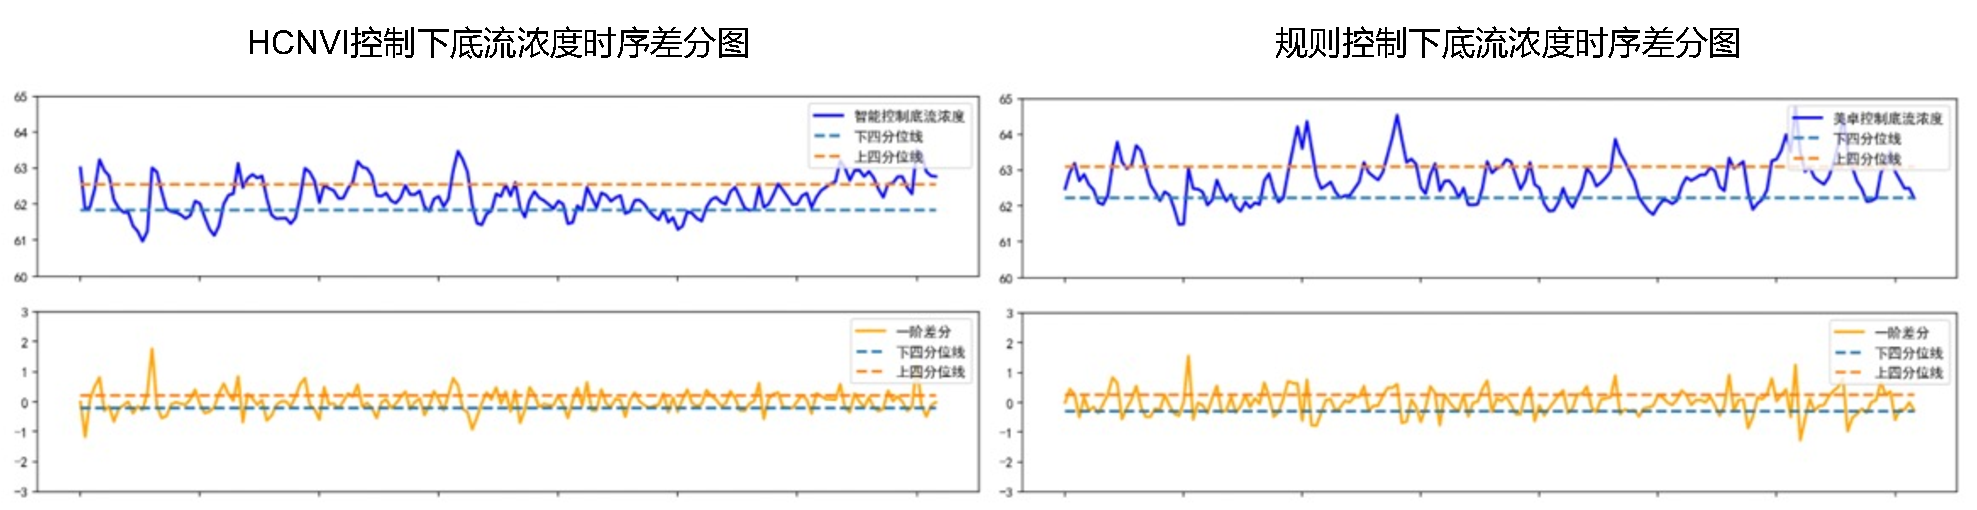
\includegraphics[width=\linewidth]{figures/chapter6/difference.pdf}
  \subfigure[HCNVI控制时底流浓度时序差分图] {
    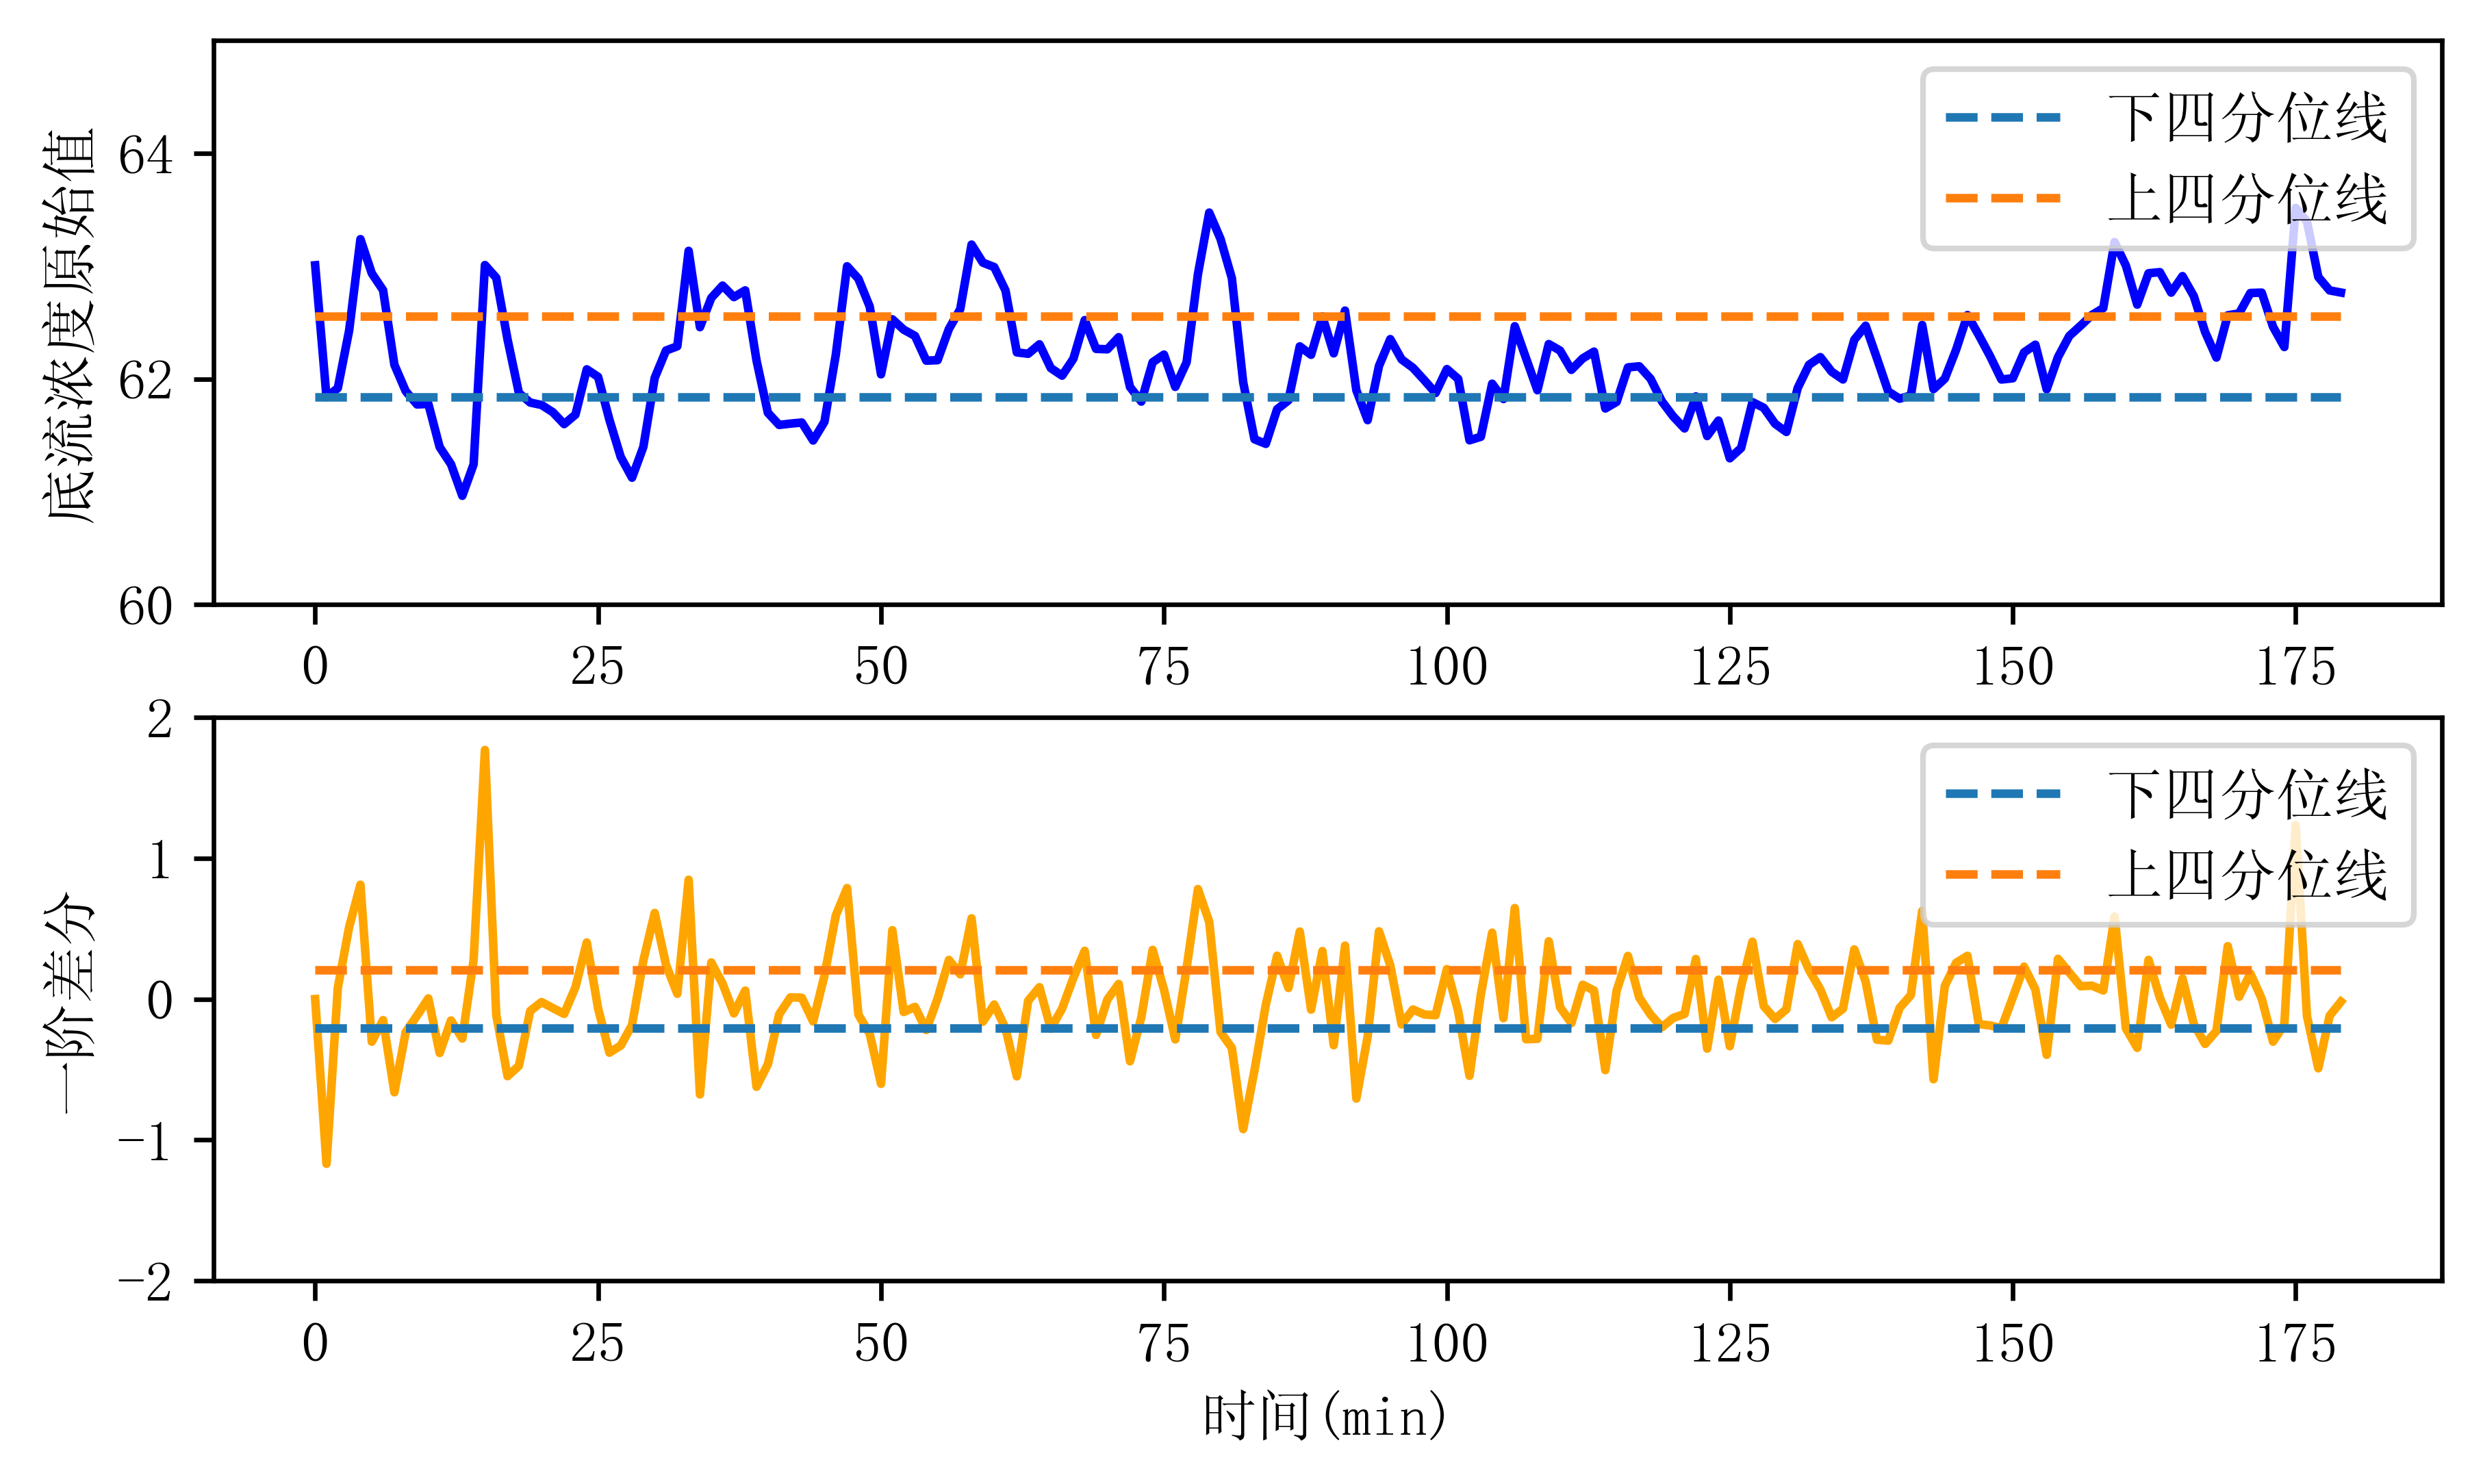
\includegraphics[width=0.48\linewidth]{figures/chapter6/intelligent_diff.png}}
  \subfigure[规则控制时底流浓度时序差分图] {
    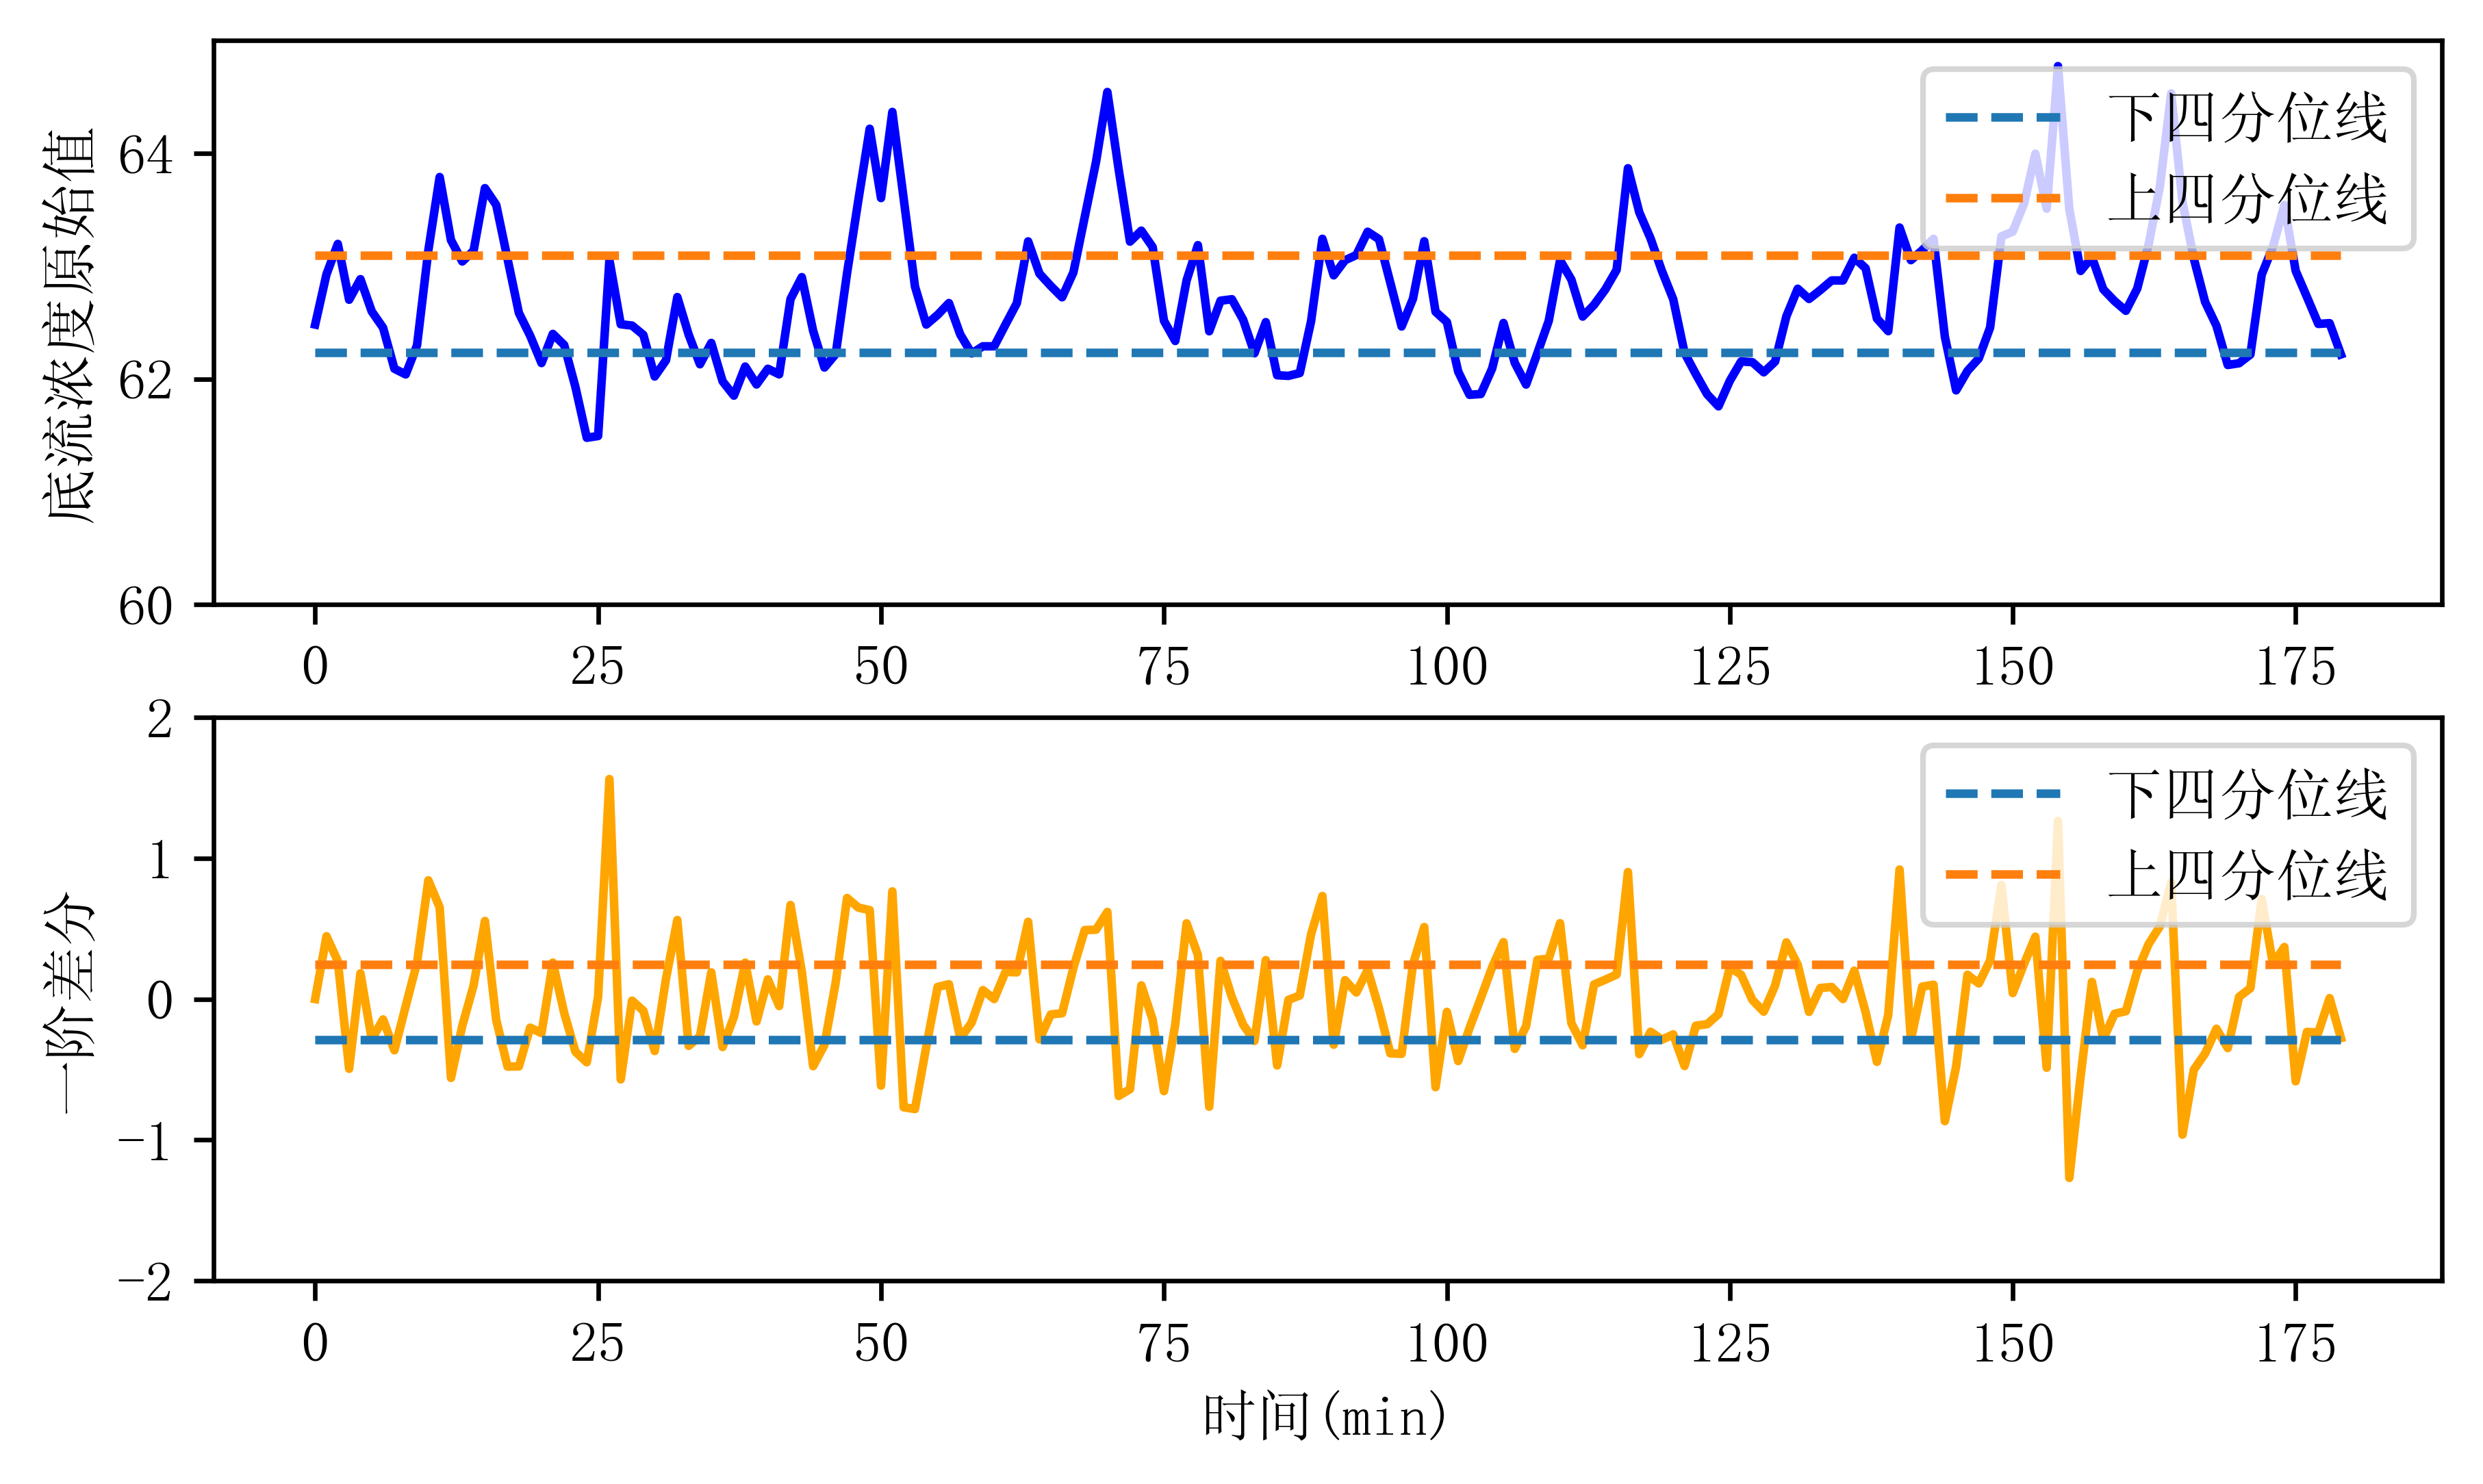
\includegraphics[width=0.48\linewidth]{figures/chapter6/mesto_diff.png}
    }
  % \label{fig:6_concentration_diff}
  \caption{底流浓度控制差分对比图}
  \label{fig:difference}
\end{figure}
从图中可以看到,HCNVI控制下的底流浓度的上四分位点与下四分位点之间的间距明显小于规则控制的间距,说明整体追踪控制精度更佳。对于底流浓度的一阶差分序列,HCNVI控制下的四分位线间距距为0.4142,略小于规则控制的0.5331,本章方法下底流浓度的控制稳定性更优。

与此同时,我们将图\ref{fig:difference}所示的底流浓度数据进行时间序列分解,比较残差项的四分位距受控制算法的影响,对比结果如图\ref{fig:decompose}所示。从图中可以看到HCNVI控制算法下,残差项序列的波动较小且更接近0,四分位居(0.4267)略小于规则控制四分位距(0.6836),
\begin{figure}[htb]
  \centering
  \subfigure[HCNVI控制时底流浓度序列残差分解图] {
    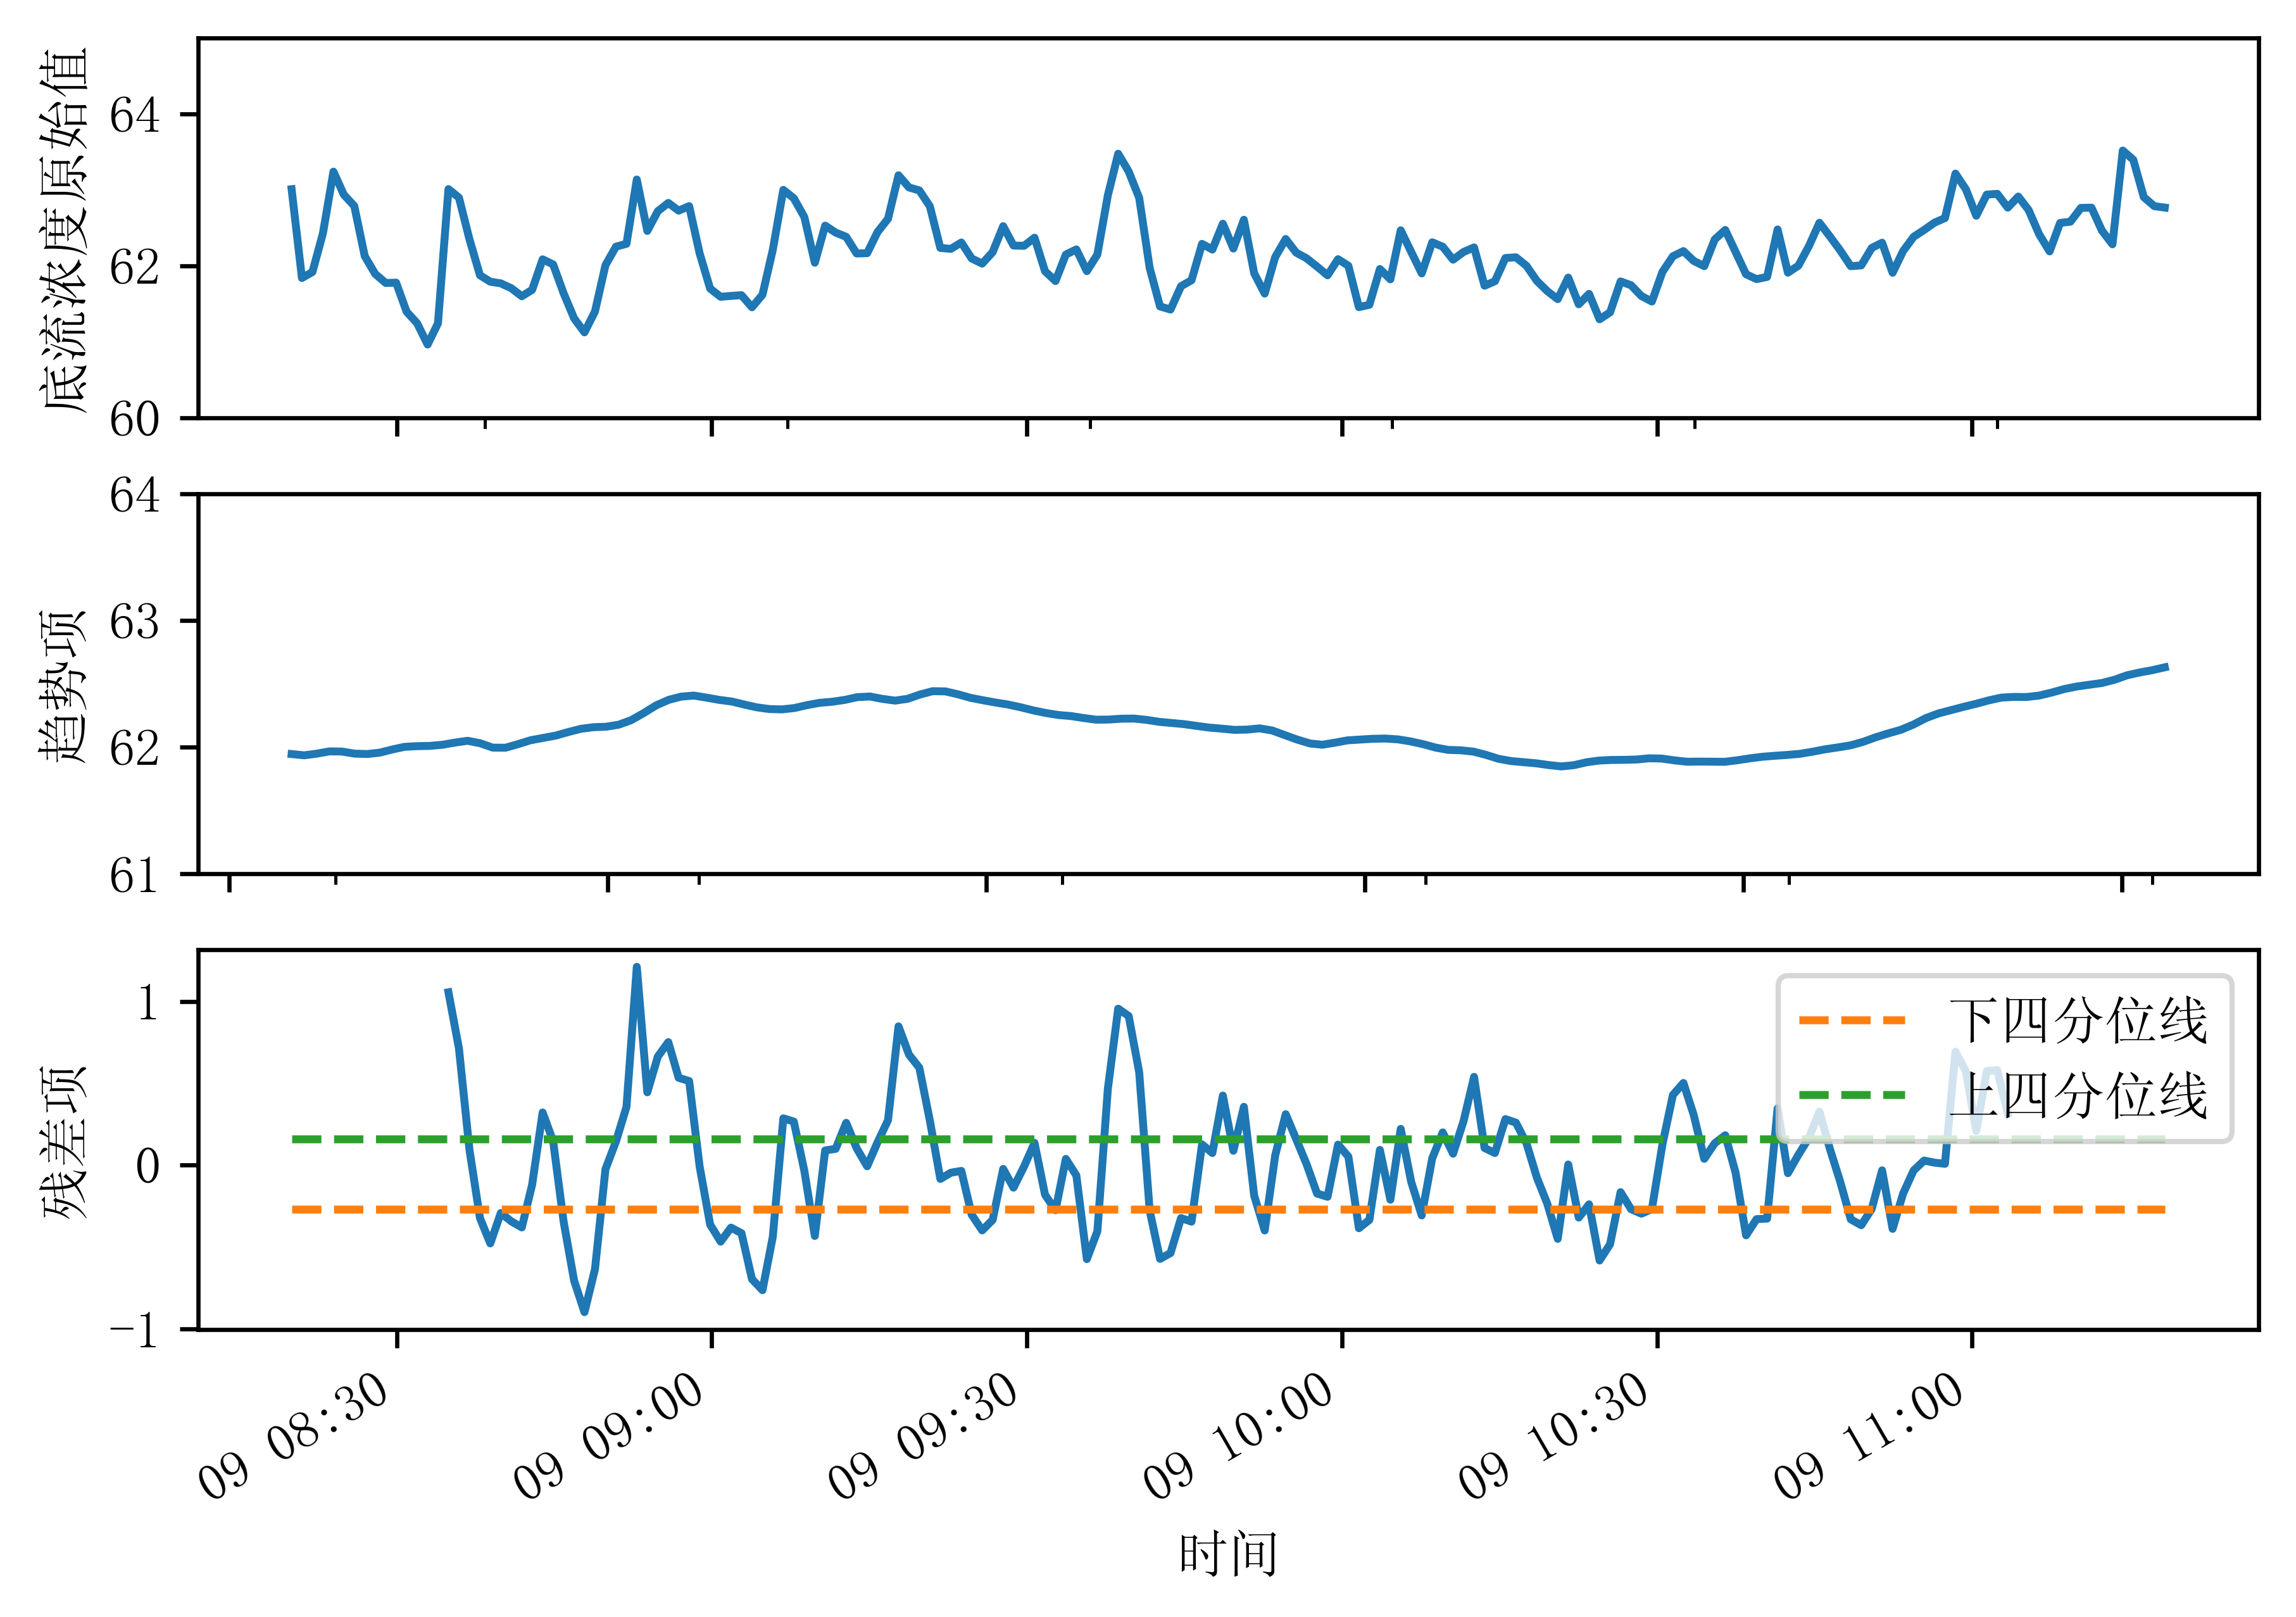
\includegraphics[width=0.48\linewidth]{figures/chapter6/intelligent_season.png}}
  \subfigure[规则控制时底流浓度序列残差分解图] {
    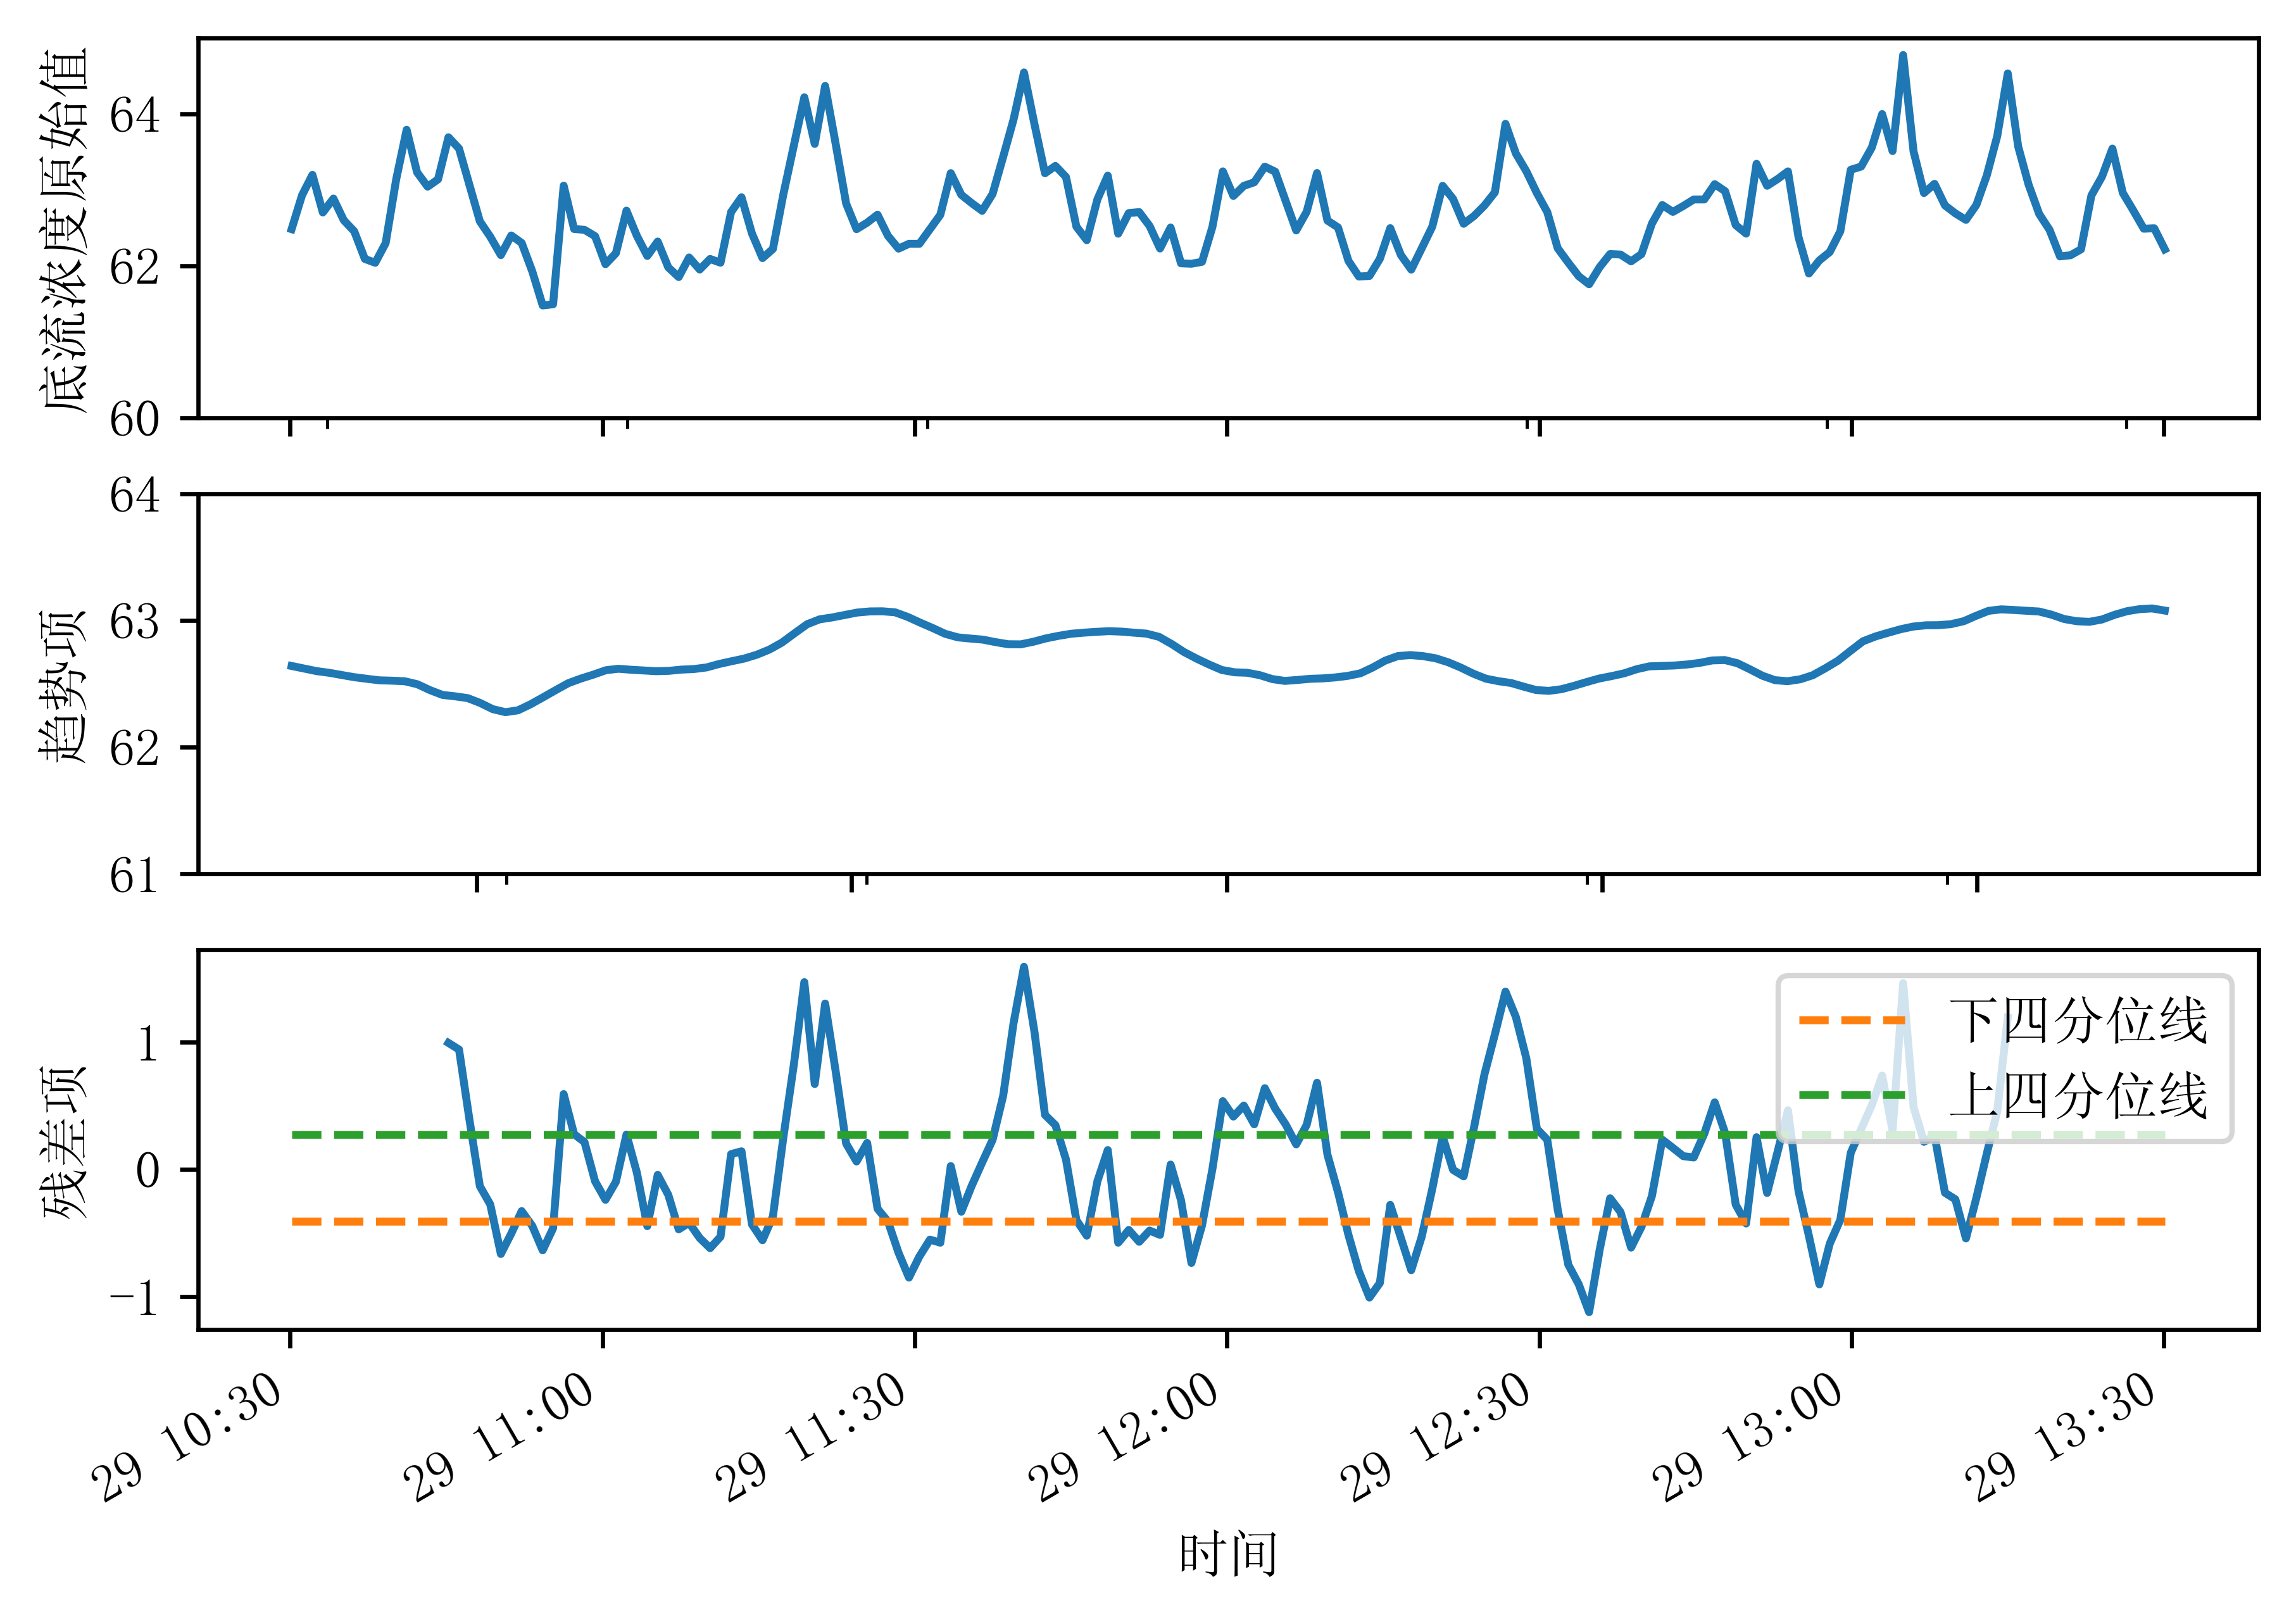
\includegraphics[width=0.48\linewidth]{figures/chapter6/mesto_season.png}
    }
  \caption{底流浓度序列残差分解对比图}
  \label{fig:decompose}
\end{figure}
% \tabref{tab:dis_decompose}对比了两种控制算法季节项和残差项的四分位距。结果说明系统在HCNVI算法的控制下的底流浓度能够整体保持稳定,且波动更小。
% Table generated by Excel2LaTeX from sheet 'Sheet1'
% \begin{table}[htb]
%   \centering
%   \caption{引入智能控制算法之后的底流浓度稳定性对比}
%     \begin{tabular}{cccc}
%     \toprule
%     \multicolumn{2}{c}{\textbf{自研智能控制算法}} & \multicolumn{2}{c}{\textbf{美卓控制算法}} \\
%     \midrule
%     季节项四分位线距离 & 0.2007 & 季节项四分位距 & 0.2165 \\
%     \midrule
%     残差项四分位线距离 & 0.4267 & 残差项四分位距 & 0.6836 \\
%     \bottomrule
%     \end{tabular}%
%   \label{tab:dis_decompose}%
% \end{table}%

另外,为了进一步说明该控制算法对于浓密机运行过程的控制能力,本节测试并观察了了控制算法在开闭前后的浓度变化情况。如图\ref{fig:actual}所示:

\begin{figure}[htb]
  \centering
  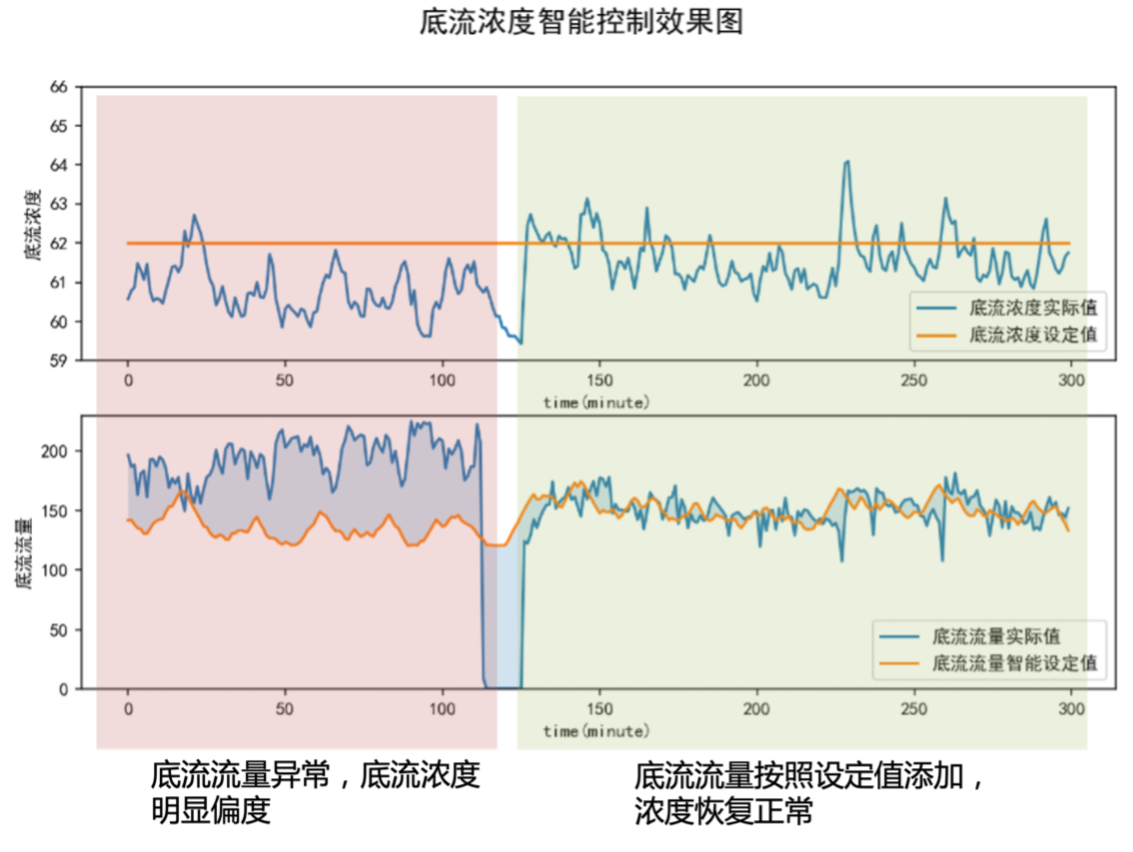
\includegraphics[width=\linewidth,trim=0 0 0 2,clip]{figures/chapter6/actual.png}
  \caption{开启智能控制前后浓密机底流浓度变化对比}
  \label{fig:actual}
\end{figure}
在红色区域内,底流流量明显高于设定值,造成了浓密机屯料过少,底流浓度远低于预期值(62\%)。在绿色区域内,底流流量图中的蓝色与橙色线较为接近,说明启用了控制算法给出的流量设定值。此时底流浓度不断升高,到达设定点附近震荡。该实验充分验证了本章控制算法对于浓密机底流浓度的追踪控制是有效的。











% Table generated by Excel2LaTeX from sheet 'Sheet1'

% \subsection{基于常微分方程网络的隐空间变分推理}
% \subsection{基于随机微分方程网络的受控系统生成模型}
% \subsection{基于连续时间隐空间超调预测的长期预测性能优化}
% \section{连续时间非确定性模型在深锥浓密机系统预测中的应用分析}
% \subsection{数据集描述}
% \subsection{非确定性模型与确定性模型的预测性能对比}
% \subsection{连续时间隐空间超调预测对于长期预测性能的改进分析}



%}
\section{本章小结}
\label{sec:conclusion}
本章提出了基于连续时间有模型强化学习的自适应控制算法HCNVI,该算法通过构建用于识别系统动态方程的模型网络以及用于估计折扣积分代价的评价网络来解决复杂系统优化控制问题。
该方法可以在对被控系统未知的情况下,仅利用被控系统输出数据以及历史运行数据即可实现在线学习并获得较好的控制效果。
另外本章提出的短期经验回放技术可以很好地增强评价网络训练的稳定性,在其他自适应动态规划算法中也具有较好通用性。
根据仿真实验验证结果可以发现,相比其他在线ADP算法,由于HCNVI算法模型结构简单,且具有较高的学习敏捷性,因此消耗了更少的训练时间但获得了更优的控制效果。
% 但是HCNVI算法也存在自身的局限性,其去掉动作网络的可行性是建立在控制频率较高,系统运行稳定且满足利普希茨连续的特性基础之上的。
% 当被控系统相对复杂且不再具有此特性时,如系统状态量变化过程并不连续或系统运行速度较快,HCNVI依靠迭代算法求解的控制量难以保持最优性,控制性能极有可能产生退化。
% 如何使HCNVI算法以及其他无动作网络类自适应动态规划类算法适用于此类复杂被控系统,在优化训练时间消耗的同时保证其控制性能与收敛速度,将是未来非常有意义的研究方向。
% 最后,本章以
最后,本章基于HCNVI算法开发了深锥浓密机底流浓度智能控制系统并应用于某真实矿山生产场景中,现场实验表明,智能控制系统相比于原始的规则控制算法,大幅度提高了出料浓度的追踪控制精确度及控制稳定性。